\documentclass[phd,ilcc,twoside]{infthesis}
\usepackage{url}
\usepackage{xcolor}
\usepackage{graphicx}
\usepackage{textcomp}
\usepackage{xcolor}
\usepackage{color, colortbl}
\usepackage{subcaption}
\usepackage{multicol}
\usepackage{multirow}
\usepackage{array}
\usepackage{amsmath,amssymb,amsfonts}
\usepackage{makecell}
\usepackage{rotating}

\usepackage{listings}
\usepackage{subcaption}
\graphicspath{ {images/} }


\usepackage[some]{background}

\SetBgScale{1}
\SetBgContents{\parbox{14cm}{%
%\centering
\includegraphics[scale=5.2]{roundel.jpg}}}
%  \Huge Draft:  \today\\[14cm]\rotatebox{180}{\Huge Draft:  \today}}}
\SetBgColor{gray}
\SetBgAngle{0}
\SetBgOpacity{0.06}

\title{
{Traffic microstructures and network\\ anomaly detection}\\
}
\author{Henry Clausen}
\date{\today}
\submityear{\today}


\newtheorem{hypothesis}{Hypothesis}

\newtheorem{rquestion}{Research Question}

\begin{document}

\begin{titlepage}
   \begin{center}
       \vspace*{0.6cm}
 		\Huge
       \textbf{Traffic microstructures\\ and network anomaly detection}
       
		\LARGE
       \vspace{0.3cm}
        Subtitle
            
       \vspace{0.4cm}

       \textbf{Henry Clausen}

\BgThispage
       \vfill
            
\large       A thesis presented for the degree of\\
       Doctor of Philosophy
            
       \vspace{0.5cm}
     


\includegraphics[scale=0.4]{roundel_informatics.jpg}
            
\large Laboratory for Foundations of Computer Science (LFCS)\\            
\large School of Informatics\\
University of Edinburgh\\
%United Kingdom\\
\today
            
   \end{center}
\end{titlepage}

%\maketitle
%\begin{titlepage}
   \begin{center}
       \vspace*{1cm}
 		\Huge
       \textbf{Traffic microstructures\\ and network anomaly detection}
       
		\LARGE
       \vspace{0.5cm}
        Subtitle
            
       \vspace{0.8cm}

       \textbf{Henry Clausen}

%\SetWatermarkText{\includegraphics[width=\textwidth]{roundel.png}}
\BgThispage
       \vfill
            
       A thesis presented for the degree of\\
       Doctor of Philosophy
            
       \vspace{0.5cm}
     


\includegraphics[scale=0.4]{roundel_informatics.jpg}
            
\large Laboratory for Foundations of Computer Science (LFCS)\\            
\large School of Informatics\\
University of Edinburgh\\
United Kingdom\\
\today
            
   \end{center}
\end{titlepage}

%\chapter*{Abstract}
\thispagestyle{plain}
\begin{center}
    \Large
    \textbf{Traffic microstructures\\ and network anomaly detection }
        
    \vspace{0.4cm}
    \large
Subtitle
        
    \vspace{0.4cm}
    \textbf{Henry Clausen}
       
    \vspace{0.9cm}
    \textbf{Abstract}
\end{center}
Lorem ipsum dolor sit amet, consectetur adipisici elit, sed eiusmod tempor incidunt ut labore et dolore magna aliqua. Ut enim ad minim veniam, quis nostrud exercitation ullamco laboris nisi ut aliquid ex ea commodi consequat. Quis aute iure reprehenderit in voluptate velit esse cillum dolore eu fugiat nulla pariatur. Excepteur sint obcaecat cupiditat non proident, sunt in culpa qui officia deserunt mollit anim id est laborum. Lorem ipsum dolor sit amet, consectetur adipisici elit, sed eiusmod tempor incidunt ut labore et dolore magna aliqua. Ut enim ad minim veniam, quis nostrud exercitation ullamco laboris nisi ut aliquid ex ea commodi consequat. Quis aute iure reprehenderit in voluptate velit esse cillum dolore eu fugiat nulla pariatur. Excepteur sint obcaecat cupiditat non proident, sunt in culpa qui officia deserunt mollit anim id est laborum. Lorem ipsum dolor sit amet, consectetur adipisici elit, sed eiusmod tempor incidunt ut labore et dolore magna aliqua. Ut enim ad minim veniam, quis nostrud exercitation ullamco laboris nisi ut aliquid ex ea commodi consequat. Quis aute iure reprehenderit in voluptate velit esse cillum dolore eu fugiat nulla pariatur. Excepteur sint obcaecat cupiditat non proident, sunt in culpa qui officia deserunt mollit anim id est laborum. Lorem ipsum dolor sit amet, consectetur adipisici elit, sed eiusmod tempor incidunt ut labore et dolore magna aliqua. Ut enim ad minim veniam, quis nostrud exercitation ullamco laboris nisi ut aliquid ex ea commodi consequat. Quis aute iure reprehenderit in voluptate velit esse cillum dolore eu fugiat nulla pariatur. Excepteur sint obcaecat cupiditat non proident, sunt in culpa qui officia deserunt mollit anim id est laborum. Lorem ipsum dolor sit amet, consectetur adipisici elit, sed eiusmod tempor incidunt ut labore et dolore magna aliqua. Ut enim ad minim veniam, quis nostrud exercitation ullamco laboris nisi ut aliquid ex ea commodi consequat. Quis aute iure reprehenderit in voluptate velit esse cillum dolore eu fugiat nulla pariatur. Excepteur sint obcaecat cupiditat non proident, sunt in culpa qui officia deserunt mollit anim id est laborum. 

       \vfill
{\centering{\includegraphics[scale=0.4]{roundel_informatics.jpg}}}
%\justify

\chapter*{Dedication}
...

\chapter*{Declaration}

I declare that this thesis was composed by myself, that the work contained herein is my own except where explicitly stated otherwise in the text, and that this work has not been submitted for any other degree or professional qualification except as specified. Some of the material used in this thesis has been published in the following papers:

\begin{itemize}
\item Henry Clausen, Robert Flood, and David Aspinall: ``Traffic generation using containerization for machine learning''. In: \textit{Proceedings of the \textcolor{red}{abc}} (appears in Chapter \ref{Chap:Req}). 
\item Henry Clausen and David Aspinall: ``Examining traffic microstructures to improve model development''. In: \textit{2021 IEEE Security and Privacy Workshops (SPW)} (appears in Chapter \ref{Chap:Prob}).
\item Henry Clausen, David Aspinall, and Rober Flood: ``Controlling network traffic microstructures for machine-learning model probing''. In: \textit{Proceedings of the 17th EAI SecureComm Conference, Canterbury, UK, September 2021} (appears in Chapter \ref{Chap:Prob}).
\item Henry Clausen, Gudmund Grov, Marc Sabate, and David Aspinall: ``Better Anomaly Detection for Access Attacks Using Deep Bidirectional LSTMs''. In: \textit{Machine Learning for Networking: Third International Conference (MLN), Paris, France, November 24–26, 2020, Springer}  (appears in Chapter \ref{Chap:CBAM}).
\item Henry Clausen, Gudmund Grov, and David Aspinall: ``CBAM: A Contextual Model for Network Anomaly Detection''. In: \textit{Computers 10.6 (2021) (MPDI)} (appears in Chapter \ref{Chap:CBAM}).
\item Henry Clausen, Michael S. Gibson, and David Aspinall: ``Evading stepping-stone detection with enough chaff''. In: \textit{International Conference on Network and System Security (NSS), Melbourne, Australia, November 25-27 2020, Springer} (appears in Chapter \ref{Chap:NSS}).
\end{itemize}

\hspace*{0pt}\hfill Henry Clausen

\chapter*{Acknowledgements}
I want to thank...

\tableofcontents
%\listoffigures
%\listoftables

\chapter{Introduction}

A significant threat to today's computer networks are attacks that aim to gain unauthorised access to sensitive infrastructure and information, especially as the increasing rate of zero-day attacks \cite{zeroday} threatens the traditional model of signature-based network intrusion detection. Such attacks are used to gain control or access information on remote devices by exploiting vulnerabilities in network services, and are involved in many of today's data breaches \cite{mandiant2015trends}.
Anomaly-based intrusion detection methods are aimed to decrease the threat of zero-day attacks by not relying \textcolor{red}{...} on libraries of known attack signatures, but their success is currently restricted to the detection of high-volume attacks using aggregated traffic features. Recent evaluations show that the current anomaly-based network intrusion detection methods fail to detect remote access attacks reliably \cite{nisioti2018intrusion}. 

Prominent network intrusion detection methods as Kitsune \cite{mirsky2018kitsune} or DeepCorr \cite{nasr2018deepcorr} learn structures in the sizes, flags, or interarrival times (IATs) of packet sequences for decision-making. These structures reveal information about attack behaviour, but are also influenced by a number of other factors such as network congestion or the transmitted data. We define \textbf{traffic microstructures} as reoccurring patterns in the metadata of packet sequences (such as used in shallow packet inspection) within a connection, such as the packet sizes of a Diffie-Hellman exchange or typical IATs of video streaming, or patterns within the summary statistics of individual connections or short sequences observed on a host such as the pattern of port 53 (DNS) connections being followed by port 80 or 443 connection (HTTP/S). No effort has been made so far to monitor or control these factors to probe these models for specific microstructures, with the current quasi-benchmark NID-datasets pay more attention to the inclusion of specific attacks and topologies rather than the documentation of the generated traffic. 
This situation has so far led researchers to often simply evaluate a variety of ML-models on these datasets in the hope of edging out competitors, without understanding model flaws and corresponding data structures through targeted probing.
Sommer and Paxson \textcolor{red}{citation} have already \textcolor{red}{should this be in?}



%Network intrusion detection models such as DeepCorr or Kitsune \textcolor{red}{citation} increasingly rely on learning \textcolor{red}{traffic microstructures} that consist of pattern sequences in features such as interarrival time, size, or packet flags. However, there exist \textcolor{red}{little to no} research that examines common variations of benign traffic microstructures, and how attacks commonly perturb them. \textcolor{red}{Something about datasets incsufficient}. 

The aim of this thesis is to improve the understanding of traffic microstrucutres and their shaping, and to define and propose methodologies to develop machine-learning based anomaly detection methods that leverage traffic microstructures effectively.



\section{Central Research questions}\label{Sec:Reseach_questions}

\begin{rquestion}\ \\ 
How well-structured is the space of microstructures observed in the traffic of a machine or a network? To what degree are these microstructures a result of specific computational activities that are of interest for traffic classification and intrusion detection, and how much are they affected by other external variables?
%does noise or input variation blur the observable contextual differences between clearly distinct actions?

%\begin{enumerate}
%\item How can we scientifically quantify closeness between individual actions, and does it translate into the similarity of corresponding traffic structures? 
%\end{enumerate}
\end{rquestion}



\begin{rquestion}\ \\
To what degree can relevant microstructures in network traffic be captured in a model from a training dataset, and how can we achieve this? How can a model adapt to changes of structures in benign traffic?
%\begin{enumerate}
%\item Which parts of network traffic both contain important information and can be represented by a model?
%\item Can be combine models that act at different traffic levels to enhance the amount of context given by the data? 
%\item Can we efficiently disentangle overlaying network flows to isolate otherwise distorted flow groups corresponding to similar actions? 
%\item What is an efficient and realistic way to incorporate other data sources into the modelling procedure? How can this input enhance the learning process and the representation detail of a traffic model? 
%\item How can a model adapt to changes of normal contextual structures?
%\end{enumerate}
\end{rquestion}

\begin{rquestion}\ \\
What is a meaningful representation of traffic microstructures? What requirements must a labelled traffic generation framework fulfill to provide realistic data?
%\begin{enumerate}
%\item What requirements must a labelled traffic generation framework fulfill to provide realistic data?
%\item Can we evaluate the traffic representation of a model through its ability to identify contextual closeness between traffic instances correctly?
%\item How can we quantify the capability of a given traffic model to identify new computational actions on a machine?
%\end{enumerate}
\end{rquestion}


\begin{rquestion}\ \\
What will a contextual model be able to prevent? 
%\begin{enumerate}
%\item What kind of attacks will necessarily show contextual anomalies, and which will not?
%\item Can an adversary adapt his attacks to avoid detection? How can we prevent this?
%\end{enumerate}
\end{rquestion}



\section{Motivation}

This section motivates the research on traffic microstructures and corresponding models and generation processes.

\subsection{The case for machine learning and anomaly-based intrusion detection}

Intrusion detection can be seen as a never ending arms-race between malicious actors on the one side that aim to access, manipulate, or damage computation infrastructure in a network, and the network operators, detection system providers and research community, on  the other. Traditionally the most common approach to network intrusion detection is based on detecting closely defined notions of attacks, known as \emph{attack signatures}. Since the late 1980's, signature based systems such as Snort or Bro \textcolor{red}{citation} have dominated the field of network intrusion detection due to high effectiveness, low false positive, and good computational efficiency. Due to their design, signature-based methods can only alert on known issues that had been categorised as threats on a signature list; zero-day attacks remain a \textcolor{red}{large vulnerability} of traditional IDSs.

In the 1990's, anomaly-detection emerged as a complementary detection tool by training machine learning or statistical analysis on large traffic datasets in order to detect variants on existing attacks or entirely new classes of attacks. However, inconsistent detection results and high false positive rates lead many administrators to believe machine-learning based intrusion detection to be unreliable, computationally too expensive, and headed for a slow death.
In 2010, Sommer and Paxson discuss a number of reasons why machine-learning based detection methods failed to provide similar levels of success as their signature-based counterpart.

However, ...

Machine-learning and anomaly-based intrusion detection solutions are finding more widespread industrial application in products from companies such as Crowdstrike, Darktrace, \textcolor{red}{citation}. Furthermore, the rise of cloud computing has shifted the computational burden of complex intrusion detection systems from the monitored hosts to the cloud.


\subsubsection{SPI and microstructures}

Many ISP solutions rely on \emph{deep packet inspection} (DPI), where payloads of packets are scanned for attack signatures or anomalies. While this offers a direct view at the content of communications, it raises several problems: The computational overhead of DPI is large and scales directly with the amount of transferred data. Furthermore, DPI infringes user privacy when scanning the content of messages, potentially allowing the operator to access the vast amount of personal information sent over the internet. Finally, DPI is incapable of processing encrypted traffic, an issue that malicious actors increasingly exploit. \textcolor{red}{Some IDS-providers have started to decrypt any transferred traffic in a man-in-the-middle manner, but the ethical legitimacy of such approaches are at the very least controversial.}

\emph{Shallow packet inspection} (SPI) in contrast only inspects packet headers and is therefore computationally less expensive as well as robust against encryption and to some degree application evolution \textcolor{red}{citation}. SPI is used both by rule- and signature-based systems such as Snort, as well as by an ever increasing number of machine-learning based methods that attempt to make broad generalities about traffic solely from evaluating packet headers. \textcolor{red}{insert some statistic how many}.

For this, many traffic classification and anomaly-detection approaches leverage small-scale structures visible in the sizes, interarrival times, flags, port, etc. of packet sequences, which we call \emph{traffic microstructures}. \textcolor{red}{insert image and example here}. 

However, there exists no systematic description of these structures, and their usage is mostly only justified from high-level argumentation without any examination about the influences on them or their prevalence in the respective datasets used for evaluation. \textcolor{red}{some additional arguments about model development?}


\subsection{Lack of model development in NID}


\subsection{Dataset problems and lack of labels}




Newer models clearly leverage microstructures

However, traffic opaque 

...

\section{Contributions}

This thesis provides extensive examinations of the necessary requirements on traffic generation and traffic microstructures to enable the effective training and improvement of anomaly detection models. The here presented findings provide \textcolor{red}{...}

More specifically, we examine how current machine-learning based SPI-detection methods are designed and their requirements on comprehensive and realistic datasets to generate models that generalise well on persistent traffic microstructures. We establish our findings with several experiments and empirical evidence of shortcomings from existing datasets\textcolor{red}{...}.

This thesis then proposes DetGen, a traffic generation paradigm to provide control over various influence factors that shape traffic microstructures. The goal of DetGen is to provide researchers with extensive ground truth information and enable the generation of customisable, scalable, and controllable datasets with realistic levels of microstructure diversity. We examine with the level of control DetGen provides with a number of experiments to compare with existing traffic generation techniques. 

We demonstrate the benefit of precise traffic control and corresponding ground truth labels by probing two state-of-the-art (SOTA) NID models to understand where they fail and how they can be improved. We identify design flaws with regards to specific microstructures, and can correspondingly improve the detection performance by several percentage points. These examinations also serve as examples how the model development process in NID can be \textcolor{red}{extended} to improve existing models and build up on previous results.

Building up from these results, we propose CBAM, an anomaly detection model that detects low-volume access attacks as deviations from \textcolor{red}{persistent} flow microstructures. CBAM is trained as a self-supervised traffic language model and outperforms current state-of-the-art methods by \textcolor{red}{xxx points}. We examine persistent microstructures that are perturbed by specific attacks, and how CBAM detects these perturbations. The output of CBAM also provides valuable insights into the frequency, clustering, and evolution of microstructures in real-world traffic.

Lastly, we examine how attackers can perturb traffic in a stepping-stone attack in an adversarial way to prevent models from identifying the corresponding microstructures. We use DetGen to generate controllable stepping-stone attack data to identify which level of perturbations are required to prevent detection. We then evaluate several models with different detection methodologies on this data and conclude that realistic adversarial perturbations can evade all current methods.

\subsection{Thesis overview}

\paragraph{Chapter 2} provides the reader with background information on network traffic and attacks, machine-learning based network intrusion detection and explains the necessary concepts of machine-learning based anomaly detection for sequential data streams. The chapter highlights important NID models that leverage traffic microstructures, and discusses existing datasets and synthetic traffic generation as well as their current shortcomings, as well as related studies on traffic structures.

\paragraph{Chapter 3} introduces DetGen, a framework that provides small-scale traffic generation specifically aimed for machine-learning based intrusion detection. The chapter starts with the identification of four major shortcomings of existing NID-datasets regarding the training of machine-learning models that leverage traffic microstructures. The chapter then defines four requirements that a machine-learning-focused traffic generation framework must fulfil. The chapter then provides results from several experiments to demonstrate the lack of model \textcolor{red}{generalisability} when trained on data not meeting these requirements. 

\paragraph{Chapter 4} builds up on the results in Chapter 2 by experimentally examining the influence of several factors on traffic microstructures and the level of control that DetGen provides. The chapter then provides two case-studies on how to produce traffic effectively to probe a state-of-the-art traffic classifier, and why a certain degree of generative determinism is required for this to isolate the influence of traffic microstructures. 

\paragraph{Chapter 5} introduces CBAM, an anomaly detection model that detects low-volume access attacks as deviations from \textcolor{red}{persistent} flow microstructures. The chapter explains the reasoning for CBAM's design in order to learn specific microstructures in a self-supervised manner, and how attacks perturb these microstructures. The chapter then provides detection results and a comparison to three benchmark (SOTA) models, before examining long-term stability of the learned structures and current shortcomings on real-world datasets.

\paragraph{Chapter 6} explains the procedure of a stepping-stone attack, common techniques based on SPI to detect them, and how attackers introduce perturbations to evade detection. The chapter then provides  results from data with varying degrees of introduced perturbations and the corresponding performance results of seven stepping-stone detection methods.

\paragraph{Chapter 7} concludes this thesis, provides a crictical perspective on the presented results, and gives an outlook to future work in this area.

\chapter{Background}
%\subsection{Background}

\section{Network traffic and attacks}\label{traffic}

\subsection{Traffic metadata}

Computers in a network mostly communicate by sending \textit{network packets} to each other, which contain the control information necessary for transmission, called the packet header, and the user information, called payload. Information contained in the header depends on the respective transport layer protocol (TCP, UDP, ICMP, etc.). Fig. \ref{Fig:TCPheader} displays the content of a TCP as an example.

\begin{figure}[h!]
\centering
\includegraphics[scale=0.4]{images/tcp_header.png}
\caption{Typical format of a TCP packet. Source:\scriptsize{ https://www.lifewire.com/tcp-headers-and-udp-headers-explained-817970}\normalsize}\label{Fig:TCPheader}
\end{figure}

In a monitoring setting, packets are usually captured by network routers and stored in the widespread \textit{pcap} format. In case of space shortage or privacy concerns, packet streams are often summarised into \textbf{network flows}. RFC 3697 \cite{brownlee1999traffic} defines a network flow as a sequence of packets that share the same source and destination IP address, IP protocol, and for TCP and UDP connections the same source and destination port. A network flow is usually saved containing these informations along with the start and duration of the connection and the number of packets and bytes transferred in the connection. Both data formats are used widely by NIDSs.

%Modern firewalls typically filter packets either based on the content of the payload (such as known-malicious byte-sequences), called \emph{Deep Packet Inspection} (DPI), or on the content of the headers (such as specific source ports or IP-addresses), called \emph{Shallow Packet Inspection} (SPI). In contrast to the packet header, the payload can be encrypted, a technique that makes it unreadable to any third parties and that is becoming increasingly common in modern computer networks through protocols such as TLS or SSH.

Modern firewalls and NID solutions rely extensively on \emph{deep packet inspection} (DPI), where the payloads of packets are scanned for attack signatures or anomalies such as known-malicious byte-sequences or anomalous HTTP-requests. While this offers a direct view at the content of communications, it raises several problems: The computational overhead of DPI is large and scales directly with the amount of transferred data. Furthermore, DPI infringes user privacy when scanning the content of messages, potentially allowing the operator to access the vast amount of personal information sent over the internet. Finally, DPI is incapable of processing encrypted traffic, an issue that malicious actors increasingly exploit. \textcolor{red}{Some firwall-providers have started to decrypt any transferred traffic in a man-in-the-middle manner, but the ethical legitimacy of such approaches is at the very least controversial.}

\emph{Shallow packet inspection} (SPI) in contrast only inspects packet headers and is therefore computationally less expensive as well as robust against encryption and to some degree application evolution \textcolor{red}{citation}. SPI is used both by rule- and signature-based systems such as Snort, as well as by an ever increasing number of machine-learning based methods that attempt to make broad generalities about traffic solely from evaluating packet headers. \textcolor{red}{insert some statistic how many}.

%For this, many traffic classification and anomaly-detection approaches leverage small-scale structures visible in the sizes, interarrival times, flags, port, etc. of packet sequences, which we call \emph{traffic microstructures}. \textcolor{red}{insert image and example here}.


\subsection{Network attacks}

%Sophisticated data breaches affect hundreds of million customers and inflicts tremendous financial, reputational, and logistic damage. %Cyber-security incidents increased by 38\% in 2017, and the global cost of cyber crime is estimated to reach \$2 trillion by 2019 %\citep{conteh2016rise}. The prevention of cyber crime is therefore a globally demanded necessity.
One reason for the recent rise of cyber crime is the increased use of sophisticated techniques for the attack of specific targets. Attackers use customised social engineering and custom-build malware that penetrate defensive barriers and potentially stay undetected in an infected system for an extended period of time. 



%Existing solutions to commercial intrusion detection in computer networks are often based on \textbf{detecting signatures} of previously uncovered and analysed  attacks. Examples of such signatures include  file  hashes of malicious software, blacklisted IP addresses and domain names, and characteristics of known Command-and-Control (C\&C) protocols. Detection of a signature usually indicates an imminent intrusion and triggers investigation. 



%However, with attackers becoming adept at shedding such previously identified signatures, cyber-security researchers have to find ways of quantifying malicious activity in a more robust way. 

%However, attackers are becoming more adept at shedding previously gathered signatures: A file hash can be altered by minor modifications in the program and IP and domain addresses can be switched by changing servers. A sophisticated attack will employ new, customized protocols and software that is fitted to the targeted computer infrastructure, and thus will not show any identified signatures. 

%The field of \textit{Intrusion Detection} is concerned with the development of methods and tools that identify malicious behaviour in a computer network in a more robust way. %\textcolor{red}{In this work, I will discuss existing literature concerning a sub-branch intrusion detection, that is concerned with detecting anomalous behaviour in network traffic.... network intrusion detection  and anomaly detection}

In 1980, James P. Anderson, a member of the \textit{Defense Science Board Task Force on Computer Security} at the U.S. Air Force, published the first report to introduce the notion of automated intrusion detection \cite{anderson1980computer}. In it, he defines an \textbf{intrusion attempt} or a threat as 

\begin{quote}
\textit{"\dots an unauthorized and deliberate attempt to access or manipulate information, or to render a system unreliable or unusable."}
\end{quote}

%Such attacks can be very diverse in their nature: They can be used to achieve different goals, and correspondingly exploit different types of tools and vulnerabilities. 
Very often, intrusive attacks involve some sort network communication between the victim machine(s) and a malicious agent. As this thesis focuses primaly on network intrusion and corresponding defense systems, we will take a closer look at this type of communication. A recent survey covering intrusive attacks and defense systems distinguishes five classes of malicious network traffic \cite{nisioti2018intrusion}:

\begin{enumerate}
\item \textit{DoS-attacks}: A denial-of-service attack is an attempt to remove ability of a particular computer to communicate with other machines over an extended period of time. %Such attacks are usually targeted at network servers in order to disrupt the service it is providing. 
All major types of DoS-attacks achieve this by overwhelming the target server with service requests, which are usually corrupted in a way that causes the server to bind resources unnessecarily long for each request, and thus losing its capability to process other requests. %The most prominent type of DoS attacks are SYN-floods. They exploit the TCP-handshake protocol by sending many SYN-requests to a server while ignoring the SYN-ACK response packets sent in return by the server. This causes the server to keep waiting for a response for each of the attacker's requests, and thus binds the resources of the server while being computationally very cheap for the attacker. After a certain treshold, the server will not be able to process any more requests, rendering it unusable for actual client requests.

\item \textit{Network probing/Reconnaissance attack}: The purpose of network probing attacks is to gather information about computers in a network and possibly find vulnerabilities which can be exploited in further attacks. This typically involves sending specific service requests to other computers in the network in order to gather information about this system, such as open ports or the operating system running on a machine, contained in the corresponding response packets.
%A common type of network probing attacks is \textit{port scanning}. Its aim is to gather knowledge of computers in the network than run vulnerable services, such as HTTP servers, mail servers, and so on. A port scan achieves this by sending queries to one or more network ports on one or more computers in the network. A computer on which the contacted network port is open will respond to the query and thus reveils himself. A port scan can either be vertical, during many ports on one computer are scanned, or horizontal, where the attacker scans a small number of ports on many computers in the network. 
Network probing is often an integral part in the spreading mechanism of \textit{computer worms}.

\item \textit{Access Attacks}: These are attacks that attempt to gain unauthorized access to a machine. This could both be an individual from outside gaining access to the network, or a user from inside the network accessing services or privileges outside of their authority. Access attacks are often divided into \textit{Remote-to-Local} (R2L) where a remote attacker gains access on a system over the network, and \textit{User-to-Root} (U2R), where a user illegally gains administrator access to a machine. However, many attacks fall into both categories. 

%Access attacks can be very diverse in their nature. A simple example are brute-force attacks where an attacker guesses the passwort of a user over a network service such as SSH. Other prominent and more sophisticated cases include \textit{SQL injections}, where nefarious SQL statements are passed to an entry field for execution, or \textit{buffer overflow}, in which more data is put into a buffer of a service than it can hold in order manipulate data in the memory past the buffer.


\item \textit{Data Manipulation Attack}: Also known as "man-in-the-middle", these attacks typically involve an attacker reading and manipulating information in a data stream that is not addressed to them by exploiting vulnerable or missing authentication mechanisms in the IP protocol and related applications. A common form of such an exploit is \textit{IP spoofing} where an attacker pretends to be a trusted computer by sending packets with a spoofed trusted source IP address. Similarly, vulnerabilities in digital certificates that serve as a unique identifier of a trusted computer can be used to create fake certificate and thus trick a victim into trusting the intruder carrying the faked certificate.

%Two examples of data manipulation attacks are \textit{session replay} and \textit{website impersonation}. In a session replay, the intruder captures packet sequences exchanged between two parties and modifies part of the data before forwarding it to the receiver. Here, both parties are unaware of the data manipulation and trust the authenticity of the connection. In website impersionation, a user is unknowingly redirected to a perfect copy of the website he requested. The user is then tricked to enter confidential information into a web form, which is then sent to the attacker instead of the trusted party operating the original page. 


%Data manipulation attacks are often used pass malicious code to a victim in order to gain access on its machine. An impressive example of such behaviour was demonstrated by the malware \textit{Flame}\footnote{also known as \textit{Skywiper}}: An infected host in a network sends messages to other machines running Windows advertising itself as a Windows update provider, using spoofed IP addresses and a fake Microsoft certificate and thus defeating Microsoft's authentication mechanism. Other computers were consequently tricked into receiving malicious updates from the infected host, which would then infect their machine \cite{skywiperskywiper}.



\item \textit{C}\&\textit{C traffic}: \textit{"Command and Control"} traffic denotes the communication between an infected host and a rogue agent, called the C\&C server. The data transmitted in a C\&C channel is often exfiltrated information about the environment of the infected host, or commands from the C\&C server for the victim for further operations. %Typically, C\&C communication is used for the control of one or more so called \textit{bots}, computers that can perform tasks such as network scanning, establishing connections to other machines, or participating in DoS attacks. The communication between a bot and the C\&C server is therefore extended and continuous over time. However, C\&C communication can also be used for the request and transmission of an encryption key needed in a ransomware attack, in which it is limited in time and size. 
C\&C communication is usually sent over the HTTP or HTTPS protocol as it is widely available and allows the attacker to hide their communication in the large volume of diverse traffic sent over this channel \cite{lamprakis2017unsupervised}.

\end{enumerate}

%An additional class of networking threats is the \textit{unauthorized surveillance} of network traffic. A local network of computers is usually separated from the outside, with a router establishing the connection between computers in the network and ones outside the network. The traffic exchanged between machines inside the network therefore does not leave the network and is not visible for outsiders. Unauthorised access captures of internal network traffic can give an intruder significant information about the network topology, and even access to sensitive information if a connection is not encrypted. As network surveillance usually does not leave any visible traces in the network, I did not include it in the above listed types of malicious traffic. 




\section{Anomaly detection}

Anomaly detection refers to the problem of identifying data instances that have significantly different properties than previously observed ``normal data instances. Anomaly detection has its origins in statistical research where normal data instances are assumed to be generated as random variables by a probability distribution $P_\textit{N}(X)$. New data is then identified as anomalous if its properties correspond to regions with vanishing likelihood, i.e. this particular data instance is highly unlikely to be generated by $P_\textit{N}(X)$. Usually, the hard part in anomaly detection is to use observed data efficiently to build an estimated distribution $\hat{P}_\textit{N}(X)$ that resembles $P_\textit{N}(X)$, and often rlies on training machine-learning models. 

Machine learning methods are often grouped into supervised methods trained on labelled data, and unsupervised/self-supervised methods that are trained on unlabelled data\footnote{Semi-supervised methods are sometimes identified as a separate group, but their functionality is often closely related to supervised methods.}. Besides the input data samples, supervised methods receive separate response data that the model is then trained to predict in a general settings without any available response data. Typically, the response data is a class label for the corresponding data sample, or numerical values in a regression-type problem. 
Unsupervised or self-supervised methods are trained entirely on the input samples in the absence of a separate response. For this, an artificial response is often generated from the input data by masking some variables or data samples and predicting it from the remaining variables or surrounding data samples. Since this information is usually available, the purpose is often not the prediction itself, but to extract information such as numerical thresholds, sample likelihoods, or groupings that describe the data. Examples of this are clustering methods or time-series and sequence prediction. 

Machine-learning-based anomaly-detection typically deal with a two-class classification problem, where one class, benign data samples, are abundant and coherent in their structure while the other, anomalous data samples, are rare, incoherent, and thus more difficutl to describe. Anomaly-detection methods are therefore trained in an unsupervised or self-supervised manner entirely on benign data samples to extract information on their underlying structures and provide boundaries of typical behaviour to distinguish them from anomalous samples that \textcolor{red}{exceed} these boundaries.

\begin{figure}
\centering
\begin{subfigure}[b]{0.45\textwidth}
\includegraphics[width=\textwidth]{images/outlier_mine.png}
\caption{}
\end{subfigure}
\begin{subfigure}[b]{0.45\textwidth}
\includegraphics[width=\textwidth]{images/Atrial_Premature_Contraction.png}
\caption{}
\end{subfigure}
\caption{The left plot (a) depicts simple anomalies that deviate in distance from regular data. The right plot (b) shows a contextual anomaly where a group of data instances do not follow a repeating timely behaviour with respect to all other data points (corresponding to an \textit{Atrial Premature Contraction}, taken from \cite{chandola_anomaly_2009})}\label{graph2}
\end{figure}


Real-world benign data is typically exhibits structures in a myriad of ways, and it is often impossible to build a model that reflects all of these structures in an accurate way. Even though anomaly-detection methods are often claimed to be independent of a notion of anomalous or attack behaviour, the design of the method and the choice of which structures the learned benign-boundary is generated from mean that some knowledge of how anomalous behaviour will differ from benign is needed.

Anomaly detection has found wide application in areas where stability of  critical systems or detection of their abuse is crucial. Examples of these include engine-fault detection in wind-turbines and fraud detection for credit cards. The assumption here is that the modelled system, such as the sensor-data stream of an engine or the buying behaviour of a customer, remains stable and generates consistent data.


%\subsection{Classification vs anomaly-detection}
%Supervised vs self-supervised

\subsection{Language models and self-supervised sequential training}

In natural language processing, language models are used for text completion, generation, and correction. A statistical language model is a probability distribution that describes the overall likelihood of a sequences of words. For example, in the sentence ``\textit{The students opened their laptops.}'', the language model could provide the probability 

\begin{align*}
\Pr\big(\text{\small``laptops''}|\text{\small``The students opened their''}\big)
\end{align*}

of the word ``laptop'' following the previous part of the sentence.

%\begin{figure}
%\centering
%\includegraphics[width=0.7\textwidth]{images_introduction/Langmod.png}
%\caption{Depiction of the output a language model provides on a given input.}
%\end{figure}

Language are typically trained in a self-supervised way with large amounts of unlabelled text. The model is fed an input sentence with a part of the sentence masked that the model tries to predict. The predictions are then compared to the actual words, as depicted in Fig. \ref{Fig:Langmod}.

\begin{figure}
\centering
\includegraphics[width=0.75\textwidth]{images_introduction/Langmod2.png}
\caption{Depiction of the training of a language model on a given input.}\label{Fig:Langmod}
\end{figure}

In the past, language models were mainly built using simple \textit{N-gram} models or \textit{Hidden Markov} models. In the last decade the success of deep learning pushed \textit{LSTM-based}\footnote{Long-short-term memory} networks as depicted in Fig. \ref{Fig:Langmod} to the top of well-performing language models. Recently, LSTM-networks have been overtaken by \textit{Transformer}-networks that can be trained more efficiently on huge datasets. 

Language models can be used as anomaly detectors in for example a grammar checking setting. Here, the predicted probability of a word or a whole sentence are compared to a threshold value, and grammatical or syntactical anomalies are detected as low predicted probabilities. 

Written language and network traffic metadata bear significant similarity as each consists of sequences of discrete events (words vs. packets/flows) that stand in contextual relationship to their surroundings. However, the application of successful language models to network anomaly detection is still unexplored. A part of this thesis tries to demonstrate the potential of training language models to capture traffic microstructures.

\section{Network intrusion detection}

%Sophisticated data breaches affect hundreds of million customers and inflict tremendous financial, reputational, and logistic damage. One reason for the recent rise of cyber crime is the increased use of advanced techniques for the attack of specific targets. Attackers use customised social engineering and custom-built malware that penetrate defensive barriers and potentially stay undetected in an infected system for an extended period of time. 

%Cyber-security relies on a range of defensive techniques, including sophisticated intrusion detection systems and firewalls that try to detect and prevent attacks against software subsystems. Malicious software still remains the biggest threat to computer users, and its detection is of utmost importance. 

The field of intrusion detection is concerned with the development of methods and tools that identify and locate possible intrusions in a computer network. %An \textit{intrusion detection system} (IDS) is typically a device or software application that detects malicious activity or policy violations in an automated way by scanning incoming data collected from one or more sources for patterns that a model or a set of rules classifies as potentially malicious.
Intrusion detection is a well researched area, with the first IDSs emerging in the late 1980's. Intrusion detection today comprises a variety of research areas in terms of different types of data sources, system architectures, detection sope, and so forth. Denning \cite{denning1987intrusion} in 1987 established the notion of two different types IDS implementations: a) host-based and b) network-based. 
\textit{Host-based intrusion detection systems} (HIDS) monitor each host in a network individually, and rely on local data streams such as application logs or raw operating system calls as  data source. \textit{Network-based intrusion detection} refers to the detection of malicious traffic in a network of computers and uses network traffic captures as a data source. %In this thesis, I will focus on network traffic as a data source due its universal nature, its resilience against modification, and my previous experience in the field. However, I will also investigate the possibility of relating both types of traffic. For more details on IDS implementations, I refer the reader to my more detailed literature review. 

%Current detection methods are predominantly based on the analysis of previously identified attack signatures, which provides great reliability and low false alert rates. However, these methods are dependent on an updated attack signature database and provide no protection against previously unseen attacks. With attackers having access to more resources than ever, custom-built malware is becoming more common to circumvent signature-based detection. 

%Another approach that has recently gained traction in commercial deployment is based on detecting malware and other undesired activity as anomalous behaviour when compared to benign computer activity. In this approach, known as \textbf{network anomaly detection} after Denning \cite{denning1987intrusion}, models must quantify the behaviour of normal network behaviour to be independent of a narrowly defined notion of malicious activity.

\textcolor{red}{more on how signature based methods work in comparison to ML-based}.

%\subsection{Network Intrusion Detection Systems}

%The field of intrusion detection is concerned with the development of methods and tools that identify and locate possible intrusions in a computer network. An \textit{intrusion detection system} (IDS) is typically a device or software application that detects malicious activity or policy violations in an automated way by scanning incoming data collected from one or more sources for patterns that a model or a set of rules classifies as malicious.

%Intrusion detection is a well researched area, with the first IDSs emerging in the late 1980's. Intrusion detection today comprises a variety of research areas in terms of different types of data sources, system architectures, detection sope, and so forth. Figure \ref{graph} provides a broad yet uncomplete overview of these different areas. 

%\subsubsection*{Design}

%Denning \cite{denning1987intrusion} in 1987 established the notion of two different types IDS implementations: a) host-based and b) network-based. 
%\textit{Host-based intrusion detection systems} (HIDS) monitor each host in a network individually, and rely on local data streams such as application logs or raw operating system calls as  data source. 
%\textit{Network-based intrusion detection} refers to the detection of malicious traffic in a network of computers. A network intrusion detection system (NIDS) monitors network traffic within in a network and/or between the network and external hosts for malicious activity or policy violations. Network traffic data can take different forms, a more detailed explanation is provided in Section \ref{traffic}.

\begin{figure}
\centering
\includegraphics[width=\textwidth]{images/Graphic2.pdf}
\caption{A broad overview over different aspects in an IDS}\label{graph}
\end{figure}

%Host-based systems have the advantage of working with high quality data that   are   typically   very   informative \cite{lazarevic2005intrusion}. 
%NIDS have the advantage of being plattform independent and more resiliant to attacks as detection of an infection is not done on the infected system. %In this review, I will focus on work done in the area of network intrusion detection.

%\textcolor{red}{centralised etc...}

\subsection{Misuse vs  anomaly detection}

Detection methods are the core of an IDS, and are therefore the most important design choice. Traditionally, two broad types of detection approaches are identified: a) Misuse detection and b) anomaly detection. 

Misuse detection aims at detecting a particular and well known reoccurring characteristic or pattern of a malicious behaviour. Two simple examples of such a characteristic are the large number of SYN packets sent by a host in a DoS attack, and the synchronised connection of many hosts to one server in a botnet. In misuse detection, abnormal or malicious behaviour is therefore defined first before developing a model to distinguish the defined behaviour from other traffic.

%In contrast, anomaly detection aims at building a model of normal system behaviour that is accurate enough to spot any malicious behaviour as traffic that deviates from the estimated model. Anomaly detection is principally more difficult than misuse detection since the traffic model has to incorporate potentially very heterogenuous traffic behaviours. However, it is generally acknowledged that anomaly detection is more suitable to detect new and previously unseen malicious behaviour as it makes no definite assumptions on the anomalous behaviour. Misuse detection is robust against evolution of malware as long as defined malicious behaviours do not change.

In reality, anomaly and misuse detection are not necessarily mutually exclusive, and there is a fluent passage between the two. This is because many anomaly detection approaches choose a particular set of features to be modelled with a particular threat in mind. For instance, models for the number of connections of a machine are naturally suitable for detecting DoS attacks, port scans, or Worm attacks. 

As misuse detection detection methods are aimed at detecting very specific behaviour, they usually only detect one type of malicious traffic. Areas that have been researched particularly well include botnet C\&C channel detection, DoS attack detection, and port scan detection. Areas that lack a comprehensive body of research are different types of access attacks and data manipulation attacks. These are also currently the least detected attack classes \cite{nisioti2018intrusion}.

\subsection{Evaluation methodology and common flaws}

\subsection{Related methods leveraging traffic microstructures}


%\section{Controlling traffic and corresponding microstructures}
%\section{How traffic models are susceptible to microstructures}
%Include some of the findings from the stepping stone paper here:
%\begin{itemize}
%\item How models such as DeepCorr are set up to capture sequential dependencies
%\item How they are sucsceptible to chaff, long rtts, etc.
%\end{itemize}
%\subsection{Models that rely explicitely on microstructure modelling}
%Basically traffic classifiers
%\section{Application to intrusion-detection}
%\section{Capturing traffic microstructures on a flow-level with a bidirectional LSTM}
%\section{Capturing traffic microstructures on a packet-level with a LSTM-encoder}
%\section{Thesis plan}
%In the light of the problems described in Section \ref{Sec:Problems} that we encountered in the field of anomaly-based intrusion detection, I believe that the scope of this PhD-project has to be altered slightly. As there will not be enough material directly concerning anomaly detection, the formulation of building anomaly-detection models describing software behaviour should be relaxed to general applications of ML (not just anomaly detection) in specific areas related to software defined behaviour. 
%The overall unifying theme of this PhD so far has been centered around small-scale traffic structures generated by software-defined computer interactions and applications of ML language models to it, in other words \textbf{Modelling computer interactions as a language}.
%This could be based of the reoccurring use of traffic (and potentially system/program logs) generation for machine learning. The generated traffic could then be verified as valuable by the implemented intrusion detection applications.
%All applications implemented so far except for the flow-level model are driven (in part) by our traffic generation:
%\begin{itemize}
%\item Flow-level LSTM model
%\item stepping stone detection
%\item traffic relay
%\item LSTM encoder
%\item QUIC anomaly detection
%\end{itemize}
%Overall, all these applications except for the traffic relay detection are concerned with software-defined fine-grained structures. Below, I outline the different chapters that I believe should be included in my thesis:
%\begin{enumerate}
%\item Introduction and related work
%This chapter could largely draw from the existing introduction in the research proposal as well as the extensive literature survey I conducted. Updates on the scope as well as recent developments in related work would have to be added. %This should take less then three weeks.
%\item Background: Anomaly detection and challenges in security
%This chapter outlines the motivation to use anomaly-based detection models instead of classification-based ones. It furthermore highlights why anomaly detection is more difficult in security than in other areas, and what currently prevents it from being deployed outside of academia.
%\item Background: Language models and their application to security
%This chapter briefly outlines different techniques used in language modelling,  and how they can be used to build data representation useful for anomaly-detection. It also discusses previous applications of language models in security.
%\item Data sources, datasets, and data generation with realistic small scale structures
%This chapter will draw largely on the work conducted for the DetGen traffic generation framework.
%\item Computer communication structures and the effect of malicious behaviour on them
%This chapter will describe the different structures that the different layers of software-defined communication can have on the collected data. These descriptions and their corroboration can be taken from work in each of the projects described above. Furthermore, this chapter will describe how attacks can alter these structures due to the distinct approach they are taking, and why it is worth building models that focus on small-scale traffic structures.
%\item Traffic as a language and detection models
%This chapter will describe how network traffic can be described by a language model, and how to construct anomaly-based models from it. The chapter will then proceed to describe the different approaches I worked on and their respective results:
%\begin{enumerate}
%\item Flow-based modelling
%\item Connection setup model
%\item Traffic relating to process initialisations in the QUIC protocol
%\item Detecting similarity in computer connections
%\end{enumerate}
%\item Conclusions
%\end{enumerate}

%
%\section{Temporal correlation/Semantics-based}
%
%Despite network traffic being a stream of events, most anomaly-based intrusion detection approaches neglect any temporal features. Nevertheless, malicious behaviour most often is composed of  a series  of related computer and network  events and have a distinct temporal and semantic profile \cite{ye2000markov}. As an example, an intruder using a session relay to exfiltrate information or pass malicious code generates a strong dependency between incoming packets in one connection and outgoing packets in the other connection (and vice versa) albeit the individual packets or connections resemble perfectly benign behaviour\footnote{as they are essentially two normal connections that are relayed by the intruder}. Building a model that can that can understand relations and dependencies between individual events could potentially lead to great improvements in the detection of otherwise non-anomalous attacks. 
%
%Since a machine's network traffic is the collective stream of multiple processes accessing the internet, individual traffic sequences are mixed with others, which makes the modelling of temporal dependencies a non-trivial task. In comparison to the other identified categories, research in the area of anomaly detection using temporal correlation or semantic models is sparse. 
%
%
%In 2003, \textbf{Krishnamurthy et al.} \cite{krishnamurthy2003sketch} propose a rather simple, yet efficient method for network-wide monitoring of individual key occurrences in an online fashion. For that, a sliding window approach is used to asign all keys (which here stand for individual IP addresses or network ports) a value containing the number of its occurrency. For each key, the collected values are then used to train either an \textit{ARIMA} or a \textit{Holt-Winters} method, both popular and powerful time-series forecasting models which can be trained in an online fashion. Anomalies are then identified as values with a forecasting error exceeding a certain treshold and thus indicating a sudden change in occurrency-behaviour of that particular key. This is an improvement to summarisation measures such as entropy or histograms in two ways: It provides a better resolution of individual traffic channels, enabling the detection of attacks with far less volume, and enabling the modelling of more complex temporal patterns which become apparent on a lower level. And it makes attack attribution far simpler by indicating directly the key which is subject to an anomaly. 
%
%Since traffic is usually arriving at a fast rate, it is a computationally hard and memory-consuming task to count the occurrencies of all keys simultaneously. Schweller et al.  overcome this problem using a \textit{sketch-based counting approach} which uses hash-function to direct the values of a key directly to a position in a hash table without the need to store actual key in the memory. As this process is not exact, the count value is subject to statistical variations and the authors propose an unbiased estimator. The inaccuracy of the count estimator is also preventing the authors from using a probabilistic approach to anomaly detection instead of simple tresholding. However, this approach is also only counting occurrencies and does not detect any correlated key behaviour.
%
%A great problem of the proposed framework is the fact that the key translation works only in one direction, making it impossible to associate a detected change with the corresponding key. This problem is overcome by \textbf{Schweller et al.} \cite{schweller2004reversible} who propose a reversible sketch method.
%
%\textbf{Pellegrino et al.} \cite{pellegrino2017learning} last year proposed \textit{BASTA}, a framework to mine behavioural fingerprints from network flows using \textit{timed automata learning}. An automata encodes patterns of short-term interactions of a system and is a representation of symbolic sequences, often corresponding to state transitions, which it encodes in a state transition function. Applied to network flows, an automata represents sets of events\footnote{distinguished by port,  protocol, etc.} that can follow each other in the network trace of a system. To be more specific, they used a type of probabilistic automata that works with transition probabilities and thus works in a similar way to a \textit{hidden Markov model}. Events are asigned a state corresponding to the protocol and the direction of the flow, and the quantile\footnote{of the overall distribution of the individual parameters} its duration, size, and number of packets are lying in. The authors then use this framework to create malicious fingerprints by training it on malicious traffic intermixed with normal traffic. These fingerprints are then detected on an infected host if the difference between the expected and the observed state counts drops below a treshold. 
%
%This paper is itself not developing any anomaly detection techniques, and I will not discuss the flaws of its application for malware fingerprinting. It is interesting for us as the developed automata mining techniques can also find direct application in mining normal behaviour automata and thus be used in an anomaly detection model. 
%
%
%\textbf{Noble and Adams} \cite{noble_real-time_2018, noble_correlation-based_2016} have recently proposed \textit{ReTiNa}, a tool that measures temporal changes in the correlation between individual events in order to find intrusions on individual hosts. In their approach, they estimate the correlation between the time passed between two events, also called \textit{interarrival time}, of an OD pair and the associated size or number of packets of the involved events. For this, interarrival time and the size/packet number are modelled as a bivariate gaussian distribution, and the covariance matrix is estimated using maximum-likelihood-estimation. The authors use a sophisticated online-estimation method to adapt the estimates to changes in the correlation structure, which can then be identified by comparison to an offline estimate. Anomalies are then identified as a collection of changes happening across multiple OD pairs on one host or in the entire network by simple hypothesis testing, which decreases the false-positive rate. The assumption here is that different OD pairs are independent of each other.
%
%
%A big advantage of this approach is that it is adaptive and does not need a training phase, i.e. it is not reliant on attack-free training data. The method was tested both on the LANL network flow data as well as internal data from the \textit{Imperial College Academic network}. The method found several anomalies that coincide malicious activity in the network, but a definitive conclusion whether they are related is difficult to make.
%
%\textbf{Whitehouse, Evangelou and Adams} \cite{whitehouse_activity-based_2016} modeling the number of 
%network flow and \textit{user authentication} events on individual hosts as a polynomial function of the time and day and its rarity. Anomalies are then identified using Fisher's product test statistic and the reconstruction error. The method was tested on the LANL data using the auth and the flow sources and wa able to identify persistent structures in the data. 
%
%
%\subsection{Application to stepping stone detection}
%
%Especially in larger computer networks, attackers often try use relay-like command chains, also called \textit{stepping stones}, to obfuscate their origin or access machines without external connection. In such a chain, no direct connection exists between the first and the last machine, commands are sent through one or multiple intermediate machines. Stepping stone connections are usually encrypted and are notoriously difficult to identify. Upon detection, pairs of stepping stones are a clear indication of anomalous activity. 
%
%As stepping stone detection falls much more in the field of misuse detection, I will only give a very brief overview over emplyed techniques.
%
%\textbf{Zhang and Paxson} \cite{zhang2000detecting} proposed one of the first methods for detecting stepping stones in 2000. They model relayed key-stroke packet streams as a two-dimensional ON/OFF switching process, where state changes have to occur within a certain window between the two channels. Correlation is then simply detected if the number of switches lying in this window exceeds a treshold. 
%
%
%A common assumption made when trying to find stepping stones is that packet or flow streams between different hosts in a network are almost always independent of each other, which is shown by \cite{neil2013scan}. \textbf{He and Tong}\cite{he2007detecting} model normal packet arrivals in a connection as a Poisson Process, and use the assumption of independence to derive a probabilistic distribution for the similarity of packet numbers in two channels in a time interval. P-values are then used to identify when the number of similar intervals becomes unlikely. They also show that if the ratio of chaff-packets exceeds to necessary packets in a stepping stone becomes too large, correlation is impossible to detect under the asumption of normal traffic following a Poisson distribution.
%
%
%\textbf{Neil et al.}  \cite{neil2013scan} also model normal event arrivals along an edge as a \textit{negative Binomial process} with two different rates, evolving as a hidden Markov model, and correlation in different time intervals in then used  using a likelihood ratio test to obtain p-values. In their approach, instead of testing network wide correlation, which is computationally unfeasible, testing is done on two different forms of local subgraphs, a star shape and a path-shape on selected edges. 
%
%
%\subsection{Semantic-based approaches using different data sources}
%
%Approachs that model semantic or temporal behaviour characteristics have been also been applied on host-based data streams such as \textit{system call logs} or \textit{process logs} as well. As these are mostly symbolic event streams, anomaly detection in principal works similarly as for network traffic. As these data sources have usually a more hierarchical structure of events following each other in a parent-child fashion and therefore do not suffer from overlapping signals, and it is generally easier to identify semantic structures. Notable examples include the use of deterministic automata \cite{warrender1999detecting}, Markov chains \cite{ye2000markov}, hidden Markov models \cite{yeung2003host,hu2009simple}, or \textit{recurrent neural networks}\cite{du2017deeplog}.


\section{Existing datasets}


\begin{sidewaystable}[h]
\centering
\begin{tabular}{p{2.5cm}|p{3cm}|p{2.3cm}|p{2cm}|p{3.5cm}|p{3.5cm} |p{3.5cm}}
Dataset&Format&\#hosts & Duration & Source & Attacks & Generation setup\\ \hline \hline
CICIDS-18& Pcap+ML-flows (80 features) & 30 & 5 days &Synthetic (VM+scripts)& 12 (DoS, probing, access attacks) \\ \hline
UGR-18& Flows & 30 & 6 months &Real-world (+12 days synthetic) & Probing & VM-based\\ \hline
LANL-16& Flows (only internal) & 30 & 6 months &Real-world (+12 days synthetic) & Probing\\ \hline
\end{tabular}
\caption{Summary of the most commonly used NID-datasets.}\label{Tab:NIDdatasets}
\end{sidewaystable}


In order to evaluate their ability to model the behaviour of a network and to identify malicious activity and network intrusions, new methodologies have to be tested using existing datasets of network traffic. This network should ideally contain realistic and representative benign network traffic as well as a variety of different network intrusions. However, as  network traffic contains a vast amount of information about a network and its users, it is notoriously difficult to release a comprehensive dataset without infringing the privacy rights of the network users. Furthermore, the identification of malicious traffic in network traces is not straightforward and often requires a significant amount of manual labelling work.
For that reason, only a handfull of datasets for network intrusion datasets containing real world traffic exist. There have also been some efforts to artificially creating such datasets and thus bypassing any privacy concerns. However, up to today, no artificial dataset truly resembles real network traffic in every aspect \cite{nisioti2018intrusion}.

As described in a recent survey by \textbf{Ahmed et al.} \cite{ahmed2016survey}, we can generally distinguish four different types of datassets containing network traffic:

\begin{enumerate}

\item \textbf{Real network data containing known intrusions}: 

\item \textbf{Real network data containing injected intrusions}:

\item \textbf{Real network data containing no intrusions/untruthed real network data}:

\item \textbf{Synthetic network data with/without injected intrusions}:

\end{enumerate}

%I will now describe the properties of existing datasets suitable for network intrusion detection. As this review is primarily concerned with anomaly detection models that require benign network traffic, I did not include datasets such as honeypots that mostly contain malicious traffic. A description that includes such datasets can be found in the below described survey by Ahmed et al. \cite{ahmed2016survey}.




\subsection{Real-world datasets}

\subsubsection*{Los Alamos National Laboratory, 2015 - Comprehensive, Multi-Source Cyber-Security Events \cite{akent-2015-enterprise-data}\cite{kent-2015-cyberdata1}}

In 2015, the Los Alamos National Laboratory (LANL) released a large dataset containing \textbf{network flow} traffic from teir corporate computer network, which contains about 17600 computers. The data was gathered over a period of 58 days with about 600 million events per day. The data only contains internal network connections, i.e. no flows going to or coming from computers outside the network are included. IPs and ports were de-identified (with the exception of the most prominent port), but are consistent throughout the data. Since the data stems exclusively from one corporate network, it can be assumed that it shows more homogeneity in the observed traffic patterns than  general network traffic.

Additionally, the dataset also contains other event sources which were recorded in parallel in order to give a more comprehensive look at the network, and could be very useful when investigating a detection approach that correlates multiple event sources. These sources include process events and authentication events from Windows-based computers and servers, and DNS lookup events from the DNS servers within the network. 

The dataset furthermore contains a labeled set of redteam events which should resemble intrusions. However, these events are not part of the network flow data and only contain information about the time of the attack and the attacked computer. These events apparently resemble remote \textit{access attacks}, are not described further and appear to be artificial or injected into the dataset. It is thus not certain how well they resemble actual network intrusions.


LANL released another dataset containing network flow traffic from their network in 2017 \cite{turcotte17}. This dataset is similar to the one from 2015, but spans over a longer period of time, 90 days. Furthermore, it contains no labeled malicious activity,  however that does not mean that the data is completely free of malicious activity.

\subsubsection*{UNIBS 2009\cite{UNIBS2009data}}

This dataset was collected on the campus network of the \textit{University of Brescia} on three consecutive days in 2009. The dataset contains in total 79000 anonymised TCP and UDP \textit{network flows}. 

This dataset is not directed towards intrusion detection research, but was made as \textit{ground truth data} for traffic classification. It therefore contains labels which indicate which of in total six applications generated the corresponding traffic flow. It might however still be of interest for model assessment in intrusion detection that is relying on traffic classification.

\subsubsection*{CAIDA 2016 \cite{walsworth2015caida}}

The \textit{Center for Applied Internet Data Analysis} started collecting network traces from a high-speed backbone link in 2008 with the collection still ongoing. The data is available in anonymised yearly datasets containing one hour of \textbf{packet headers} for each month. 

Since the traffic is collected from a backbone link, it is very unstructured and heterogenuous. It is furthermore not necessarily free from attack traffic. Although this dataset has been used for intrusion detection before, it is more suitable for general internet traffic analysis.


\subsubsection*{MAWI 2000 \cite{sony2000traffic}}

Similarly to the CAIDA dataset, this dataset contains \textbf{packet headers} from the WIDE backbone. It is therefore similarly unstructured, anonymised, and not free from attack traffic. Since this dataset was already collected and released in 2000, it can also be remarked that the contained traffic is too old to represent modern traffic. 


\subsubsection*{UGR 2016 \cite{macia2018ugr}}

The UGR'16 dataset was released by the University of Grenada and contains \textbf{network flow}\footnote{netflow v9} data from a spanish 3-tier ISP. This ISP is a cloud service provider to a number of companies, and thus the data comes from a much less structured network than the LANL data. It contains both client's access to the Internet and traffic from servers hosting a number of services. The data therefore contains a very wide variety of traffic patterns, an advantage emphasised by the authors. IP-adresses are consistently anonymised while network ports are unchanged. However, it is not ensured that the traffic capture is complete, i.e. that all traffic coming from and going to a particular machine is captured.

A main focus in the creation of the data was the consideration of long-term traffic evolution and observable periodicity in order to enable the testing of so called \textit{cyclostationary} traffic models. The dataset correspondingly covers a very long period, spanning from March to August of 2016, and containing about 14 GB of traffic per week. 

The data is split into a training set and a test set, with the latter containing labeled attack data. This attack data does not stem from rogue agents but is in part generated in controlled attacks on victim machines, and in part injected from previously observed malware infections. The attack data is therefore does not truly correspond to actual attacks, but achieves a high degree of similarity. The implemented attacks contain:
\begin{itemize}
\item DoS attacks (controlled attacks),
\item Port scanning (controlled attacks),
\item C\&C traffic from a botnet (injected).
\end{itemize}

The authors also acknowledge that the background traffic is not necessarily free from further attacks. In fact, three real attacks have been observed and labeled, corresponding to IP-scanning and a spam mail campaign.

\subsection{Synthetic datasets}

\subsubsection*{CTU 2013 \cite{noauthor_ctu-13_nodate, garcia2014empirical}}

The \textit{Stratosphere Laboratory} in Prague released this dataset in 2013 to study botnet detection. It consists of more than 10 million labeled \textbf{network flows} captured on lab machines for 13 different botnet attack scenarios. Additionally, the raw packets for the botnet activity is also available for attack analysis. 

The labelling in this dataset is different from other datasets as each  flow  in  the  list  is  labeled  based  on  the  source  IP  address.  In  the experiments,  certain  hosts  are  infected  with  a  botnet  and  any  traffic  arising from such a host is labeled as Botnet traffic. Traffic from uninfected hosts is labeled as Normal. All other traffic is Background, as one cannot classify it. 

A criticism of this dataset is the unrealistically high amount of malicious traffic contained in the dataset, which makes it easier to spot it while reducing false positives. Furthermore, the way normal or background traffic is generated is described only poorly and leaves the question how representative it is of actual network traffic.

\subsubsection*{UNSW-NB 2015 \cite{moustafa_unsw-nb15:_2015}}

The dataset realeased by the \textit{University of New South Wales} in 2015 contains real background traffic and synthetic attack traffic collected at the "Cyber Range Lab of the Australian Centre for Cyber Security". The data is collected from a small number of computers which generate real background traffic, and is overlayed with attack traffic using the \textit{IXIA PerfectStorm tool}. The time span of the collection is in total 31 hours.

An advantage of the collected dataset is the inclusion of both \textbf{raw packets} and \textbf{network flows} along with two other data formats containing newly engineered features. This allows a more detailed analysis of the data and possibly a better distinction between attack and benign traffic. In total, the data contains 260 000 events.

Another advantage of the data is the variety of attack data, containing a number of DoS, reconnaissance, and access attacks. However, due to the synthetical injection of these attacks, it is unclear how close they are to real-world attack scenarios.

Since this dataset is collected from a relatively small number of machines and during a limited period of time, it is furthermore unclear how suitable for capturing both the temporal evolution and the heterogeneity of real background traffic.

\subsubsection*{CICIDS 2017/2018 \cite{gharib2016evaluation}\cite{sharafaldin2018towards}}

This dataset, released by the \textit{Canadian Institute for Cybersecurity} (CIC), contains 5 days of network traffic from 12 computers. These computers all have either different different operating systems such as Windows, OSX, or Ubuntu, or different versions of the same operating system in order to enable a wider range of attack scenarios. The network  furthermore contains switches, routers, a web server, a modem, and a firewall in order to ensure a realistic network topology. The traffic data itself consists of \textbf{labeled benign and attack traffic}, and is available as 11 GB per day of \textbf{raw packets} with payloads, or as \textbf{network flows}. 

It was ensured that the data contains all traffic coming and going from individual machines. However, in contrast to other datasets, the background traffic is not directly generated through user interactions on the machine, but by using a method to profile abstract user behaviour in different traffic protocol. The purpose of this is to make the traffic more heterogenuous and to ensure that different types of behaviour are present in the data during the comparably short time span. This  However, it is not completely clear how much of the underlying structure of real traffic is lost in the process, and therefore how suitable this data is to build models of benign user activity.

The attack data of this dataset is one of the most diverse among NID datasets, as it contains a variety of up-to-date attacks, such as different types of DoS attacks, SQL-injections and Heart-bleed attack, network scanning, or botnet activity. These are not always successful in order to reflect actual attack scenarios. However, the authors did not describe very well how the data from these attacks is generated and combined with the background traffic as it is also processed through a form of profiling engine. 

\textbf{CICIDS 2018:}
This dataset is generated in a similar fashion to the CICIDS 2017 data that we used in this work. The main differences are that the CICIDS 2018 data spans over three weeks and includes in total 450 hosts, but lacks the amount of web-attacks that we require and which is present in the CICIDS-2017 dataset.

The CIC released another very similar dataset to these ones in 2012.

\subsubsection*{DARPA 1998 \cite{lippmann2000evaluating}}

The \textit{Defense Advanced Research Projects Agency} released the first major dataset to test network intrusion detection systems. The data stems from two experiments at the \textit{MIT Lincoln Laboratory} were multiple victim hosts running Unix and Windows NT were subject of over 200 attacks of 58 different types. The data spans three weeks of training and two weeks of testing data and contains \textit{raw packets} that are labeled. It was since then heavily used as a benchmark to test new detection methods. %In 2000, the original data was post-processed to reduce some of its shortcomings.

Also due to its prominence, it was heavily scrutinised and received a lot of criticism for its lack of realistic background traffic, which was generated through simulation procedure, and the presence of artifacts from these simulations in the data that could heavily skew any model relying on benign traffic. Also, the high percentage of attack traffic in the data is described as unrealistic.

Furthermore, since the dataset is now more than 20 years old, it is remarked that both the benign and attack traffic does not resemble modern network traffic anymore. 

\subsubsection*{KDD Cup 1999 \cite{cup1999data,cup1999dataset}/NSL-KDD 2012 \cite{tavallaee2012nsl}}

The \textit{MIT Lincoln Laboratory} created this dataset in 1999 by processing portions of the 1998 DARPA dataset with new labels for a competition at the conference on \textit{Knowledge Discovery and Data Mining}, and is the most widely used dataset in intrusion detection. It contains 2 million connections summaries in a new format and in total 38 attack types. This new format is essentially a form of \textbf{network flows} with a greatly increased number of features, 46 in total, which give additional details about the origin of the connection. The availability of these features in a real-world application however is in my opinion unrealistic as most of them could be mined due to the availability of parallel surveilance of the host, a Solaris-based system. However, we can see significant differences in today's operating systems which barely resemble Solaris. In addition, parallel host system surveilance usually cannot be taken for granted in a realistic network environment. Naturally, as the KDD'99 data stems directly from the DARPA dataset, it also faces the same problems and criticism. 

The \textit{Canadian Institute for Cybersecurity} postprocessed the KDD'99 data in order to address some of its shortcomings. This includes removing redundant records, balancing the size of the training and test data, and adjusting the proportion of attack traffic in the data. However, the biggest criticism from the KDD'99 and the DARPA data, the unrealistic generation of background data, still prevails.


\subsubsection*{ADFA 2013/2014 \cite{creech2014developing,creech2013generation}}

The ADFA datasets, released by the \textit{University of New South Wales}, focuses on attack scenarios on Linux and Windows systems as well as \textbf{stealth attacks}. To create host targets, the authors  installed web servers and database servers , which were then subject to a number of attacks. 

The dataset contains both attack traffic and benign traffic. However, the dataset is directed more towards attack scenario analysis and is criticised as being unsuitable for intrusion detection due to its lack of traffic diversity. Furthermore, the attack traffic is not well separated from the normal one.

\subsubsection*{ICT datasets \cite{USC2010ICT}}

The \textit{Impact Cyber Trust} releases cyber security oriented data. Its repository includes many datasets, synthetic as well as real captures, from different sources. Many datasets focus on observed attack data and thus are not directly applicable to intrusion detection. Furthermore, there is in general very little information provided that describes a dataset's origin, which makes it hard to investigate the network topology.

Among the more useful datasets are the \textit{USC datasets}\footnote{DS-062, LANDER Data, and DS-266}, which contain network traffic (both \textbf{packet headers} and \textbf{network flows}) from academic networks in the US between 2008 and 2010. The datasets are very large, with the largest one covering 48 hours and containing 357 GB of packet headers. 

\subsubsection{LITNET-2020 \cite{damasevicius2020litnet}}

The LITNET-2020 from the Kaunas University of Technology Lithuania from 2020 was collected from an academic network over a timespan of 10 months and contains annotated real-life benign and attack traffic. The corresponding network provides a large network topology with more than a million IP-addresses, and the data was collected in the form of network flows with more than 80 features. However, the dataset only contains traffic from high volume attacks such as DoS-, scanning, or worm attacks, which are not suitable to evaluate CBAM.

\subsubsection{Bo{\u{g}}azi{\c{c}}i University distributed denial of service dataset} \cite{erhan2020bougazicci}

The Bo{\u{g}}azi{\c{c}}i University distributed denial of service dataset contains both benign traffic from more than 400 users from an academic network as well as artificially created DoS-attack traffic. The dataset spans only 8 minutes and contains no access attacks.

\subsection{Generative traffic models and traffic generation}

Network traffic models and corresponding traffic generation models have been one of the cornerstones of network design and stress testing. 
The fidelity of specific generated traffic characteristics to real-world traffic depends on the purpose of the generator. Simple \textbf{performance measurement tools} such as \textit{iPerf, or Mausezahn} are used for explore network transmission reliability and efficiency, and therefore only send dummy packets that do not correspond to actual communication. The realism of network activity levels and spikes is a crucial aspect for these tools. The traffic is typically sent from a client device to a server device.

Traffic generators such as \textit{Ixia PerfectStorm} aim to test the performance and scalability of \textbf{content-aware} firewalls and similar security devices. They replay application traffic such as web traffic or video streaming as well as traffic from various attacks to test the reliability and overhead of a security device. The generated traffic therefore contains actual communication with semantically correct packet sequences and payloads, but offers little room to modify the transmitted traffic. The network setup here is similar to above.

\begin{figure}
\centering
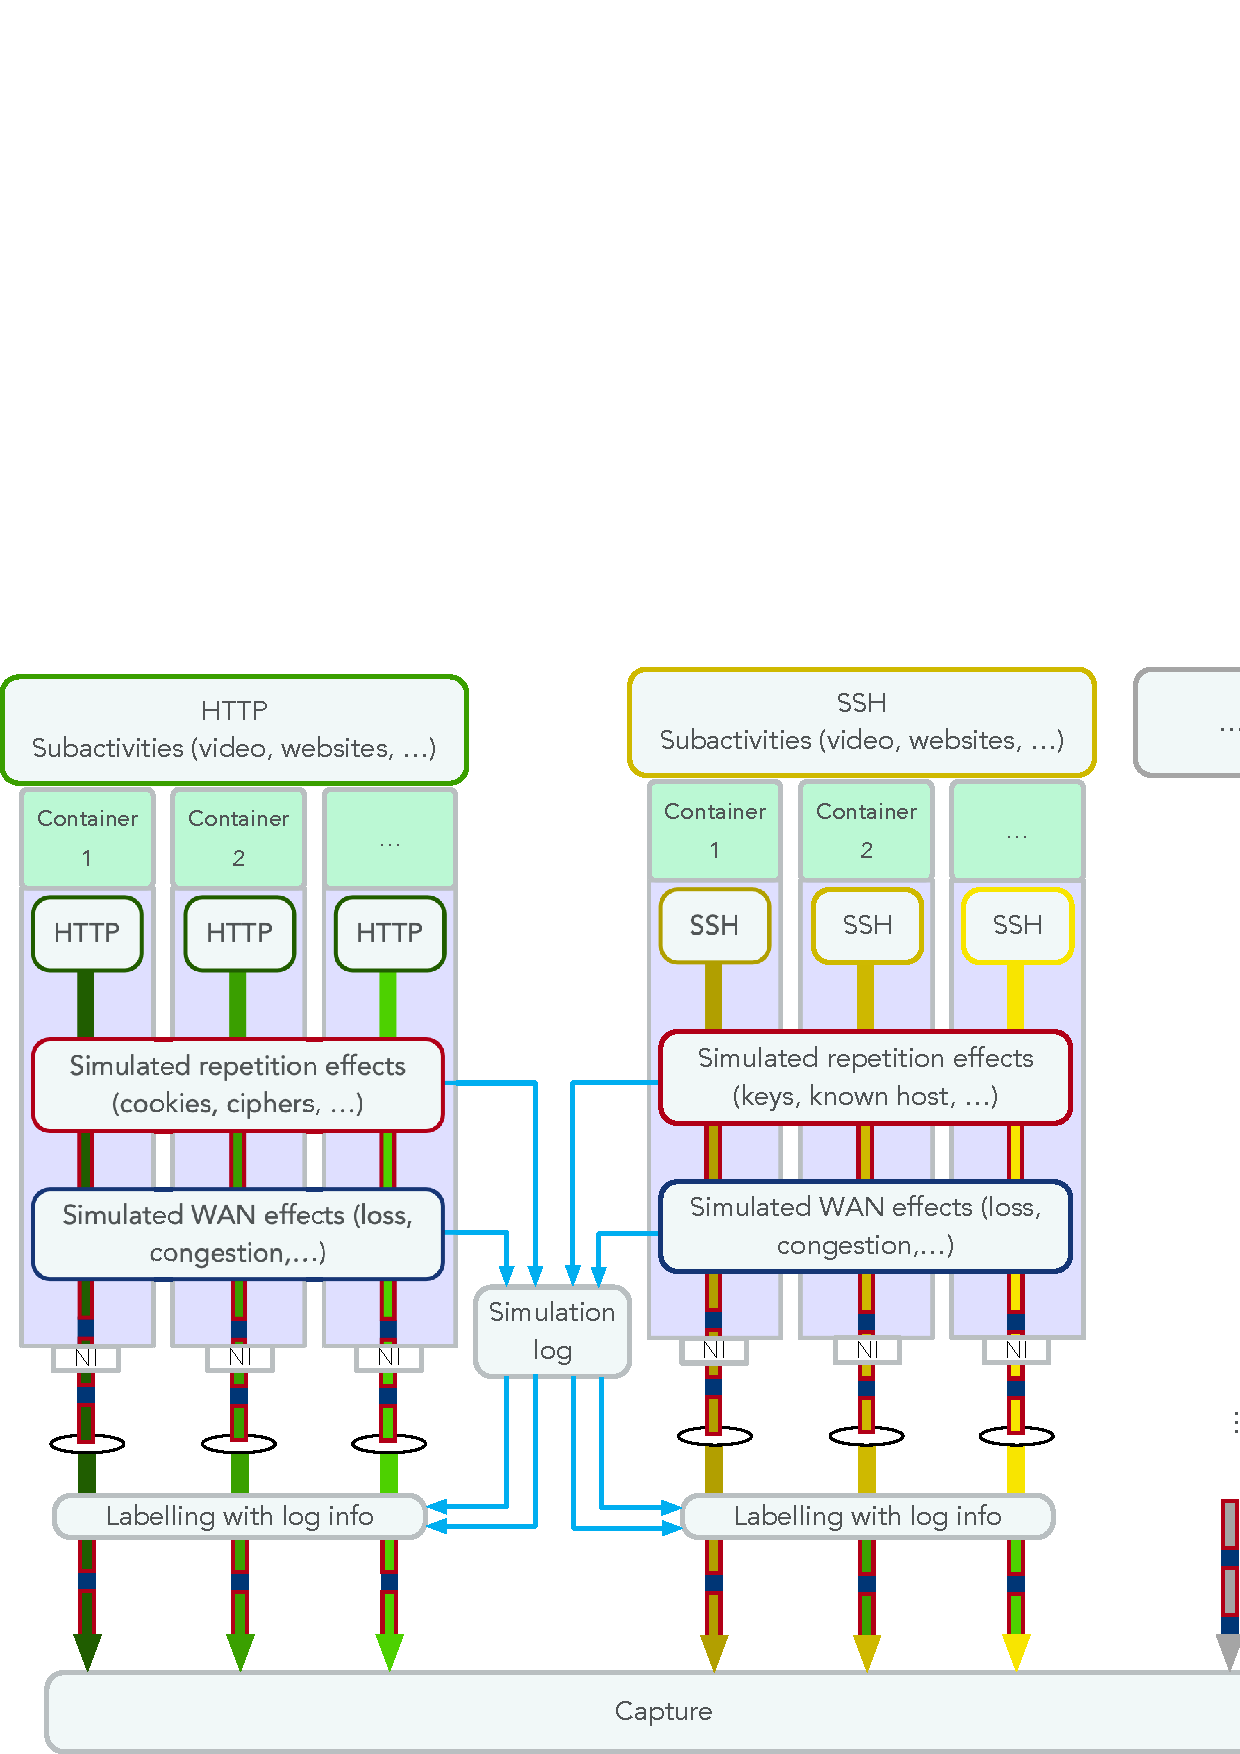
\includegraphics[width=0.7\textwidth]{images_introduction/VM_setup.png}
\caption{Setup of VM-machines in the UGR-16 dataset.}\label{Fig:VM_generation}
\end{figure}

\textbf{Traffic generation for NID-datasets} is often performed using an arrangement of virtual machines that communicate to generate traffic. The machines are configured to cover a range of network applications and protocols and communicate via scripted interactions. Attacks are typically performed from specifically designated attack machines. In Chapters  \ref{Chap:Req} and \ref{Chap:Prob}, we discuss several shortcomings of this method.

Recently, traffic emulation tools that are powered through \textbf{Generative Adversarial Networks} (GANs) such as Doppelganger \cite{lin2019generating} have attracted attention. These are trained on real-world data and are capable of generating realistic sequences of traffic features. In contrast to actual traffic generators, no actual traffic is generated and the output of GAN-models so far has been limited to numerical features such as activity levels or port entropy distributions normally obtained after traffic processing. Approaches to generate sequences of packets or flows have so far not been successful \cite{cheng2019pac,cheng2021packet}.

 





%\section{Related studies on traffic structures}



%\chapter{Related work}
%
\section{Traffic examinations}

- Paxson Sommer


- 

\section{Traffic generation frameworks}

\section{Small-scale anomaly detection approaches}




%It should address six questions:
%
%    What is the reason for writing the thesis?
%    What are the current approaches and gaps in the literature?
%    What are your research question(s) and aims?
%    Which methodology have you used?
%    What are the main findings?
%    What are the main conclusions and implications?
%

\chapter{Requirements for Machine Learning}\label{Chap:Req}

This chapter introduces DetGen, a framework that provides small-scale traffic generation specifically aimed for machine-learning based intrusion detection. The chapter starts with the identification of four major shortcomings of existing NID-datasets regarding the training of machine-learning models that leverage traffic microstructures. The chapter then defines four requirements that a machine-learning-focused traffic generation framework must fulfil. DetGen is designed to address these requirements through the use of standalone containerised communication scenarios. The majority of work in this chapter was published in \textcolor{red}{citation}.

%In the overall context of the thesis, this chapter 

Specifically important for the narrative of this thesis are:
Sect. \ref{Sec:problems} discusses problems in existing datasets, in particular regarding the lack of sufficient microstructure variation, before Sect. \ref{Sec:require} then defines requirements on the variability and monitoring of microstructures. Sect. \ref{Sec:Scenarios}, \ref{Sec:Subscenarios}, and\ref{Sec:randomsubscen} discuss in detail how these requirements can be achieved during the data generation process.

Sect. \ref{Sec:ArtiDel} performs an experimental analysis of how well the influence of real-world WAN-effects on observed interarrival times can be replicated in DetGen. Sect. \ref{Sec:DynDataGen}. Sect \ref{Sec:DynDataGen} then builds up on these results and measures the effect that differing WAN-configurations between training and evaluation data can have on a traffic classifier. 




%\section{Traffic Generation using Containerization for Machine Learning}
%
%The design and evaluation of data-driven network intrusion detection methods are currently held back by a lack of adequate data, both in terms of benign and attack traffic. Existing datasets are mostly gathered in isolated lab environments containing virtual machines, to both offer more control over the computer interactions and prevent any malicious code from escaping. This procedure however leads to datasets that lack four core properties: heterogeneity, ground truth traffic labels, large data size, and contemporary content.
%Here, we present a novel data generation framework based on Docker containers that addresses these problems systematically. For this, we arrange suitable containers into relevant traffic communication scenarios and subscenarios, which are subject to appropriate input randomization as well as WAN emulation. By relying on process isolation through containerization, we can match traffic events with individual processes, and achieve scalability and modularity of individual traffic scenarios.
%We perform two experiments to assess the reproducability and traffic properties of our framework, and demonstrate the usefulness of our framework on a traffic classification example.


\section{Introduction}


The exponential growth of data availability enabled the machine learning revolution of this decade that transformed many areas of our lives. Ironically, security oriented data describing computer networks is notoriously hard to obtain, and researchers struggle to evaluate new network intrusion detection systems (NIDS) or similar tools on suitable network traffic data.
Well-designed datasets are such a rarity that researchers often rely on datasets that are well over a decade old \cite{tavallaee2009detailed, kayacik2005selecting}, calling into question their effectiveness on modern traffic and attacks. The lack of quantity, variability, meaningful labels, and ground truth has so far slowed scientific progress and objective and appropriate measurements on ML-based network security methods.


Privacy and security concerns discourage network administrators to release rich and realistic datasets for the public. Network traffic produced by individuals contains a mass of sensitive, personal information, such as passwords, email addresses, or usage habits, requiring researchers to expend effort anonymising the dataset \cite{mirsky2016sherlock}. To examine malicious behaviour, researchers are often forced to build artificial datasets using isolated machines in a laboratory setting to avoid damaging operational devices. Background traffic is usually generated in real-time from scripts executed on the virtual machine, which constrains both the amount and heterogeneity of the data. Current experiments show that it is possible to use large network of virtual machines for traffic generation \cite{crussell2019lessons,crussell2019virtually}, however we did not find any publicly available dataset of that category. 

Existing network intrusion detection datasets are predominantly designed to support a broad range of applications, and are collected in a static manner, unable to be modified or expanded. This proves to be a serious defect as the ecosystem of intrusions is continually evolving.
Furthermore, it prohibits a more detailed analysis of specific areas of network traffic due to the available data only being a fraction of the original dataset. To combat this, new datasets must be periodically built from scratch.

Allowing researchers to create datasets dynamically to circumvent these issues would be extremely beneficial. We propose a such framework, based on application containers using Docker \cite{docker}. Docker is a service for developing and monitoring containers, also known as OS-level virtual machines. 
By moving from virtual machines to containers, we enable the scalable, modular, and dynamic creation of network traffic datasets. Since Docker containers can be arranged in complex settings with a few commands, it is a lot easier with containers to script a variety of network activities thus increase the heterogeneity and realism of the generated data.

Furthermore, each Docker container is highly specialized in its purpose, generating traffic related to only a single application process. Therefore, by scripting a variety of Docker-based \emph{scenarios} that simulate benign or malicious behaviours and collecting the resultant traffic, we can build a dataset with perfect ground truth, something that has so far not been possible for network traffic. 

Finally, the most import reason to rely on Docker for containerization is that many containerized applications are shared on the Docker Hub platform.



%This is the primary goal of this work. Furthermore, we demonstrate the utility of this framework by performing a series of experiments: one that measures the realism of the network traffic produced by our Docker scenarios and two that would be difficult to perform using a conventional dataset.

This work provides the following contributions:

\begin{enumerate}
 \item We present a novel network traffic generation framework that is designed to improve several shortcomings of current datasets for NIDS evaluation. This framework is openly accessible for researchers and allows for straightforward customization.
 \item We define four new requirements a network intrusion dataset should fulfil in order to be suitable to train machine-learning based intrusion detection methods. 
 %\item how to build new modules that can be added to the existing framework, and how this procedure enables data generation that is more suitable for data-driven methods than currently available datasets.
 \item We perform a number of experiments to demonstrate the suitability and utility of our framework. 
\end{enumerate}

\subsection{Outline}

The remainder of the paper is organized as follows. Section \ref{Sec:background} discusses existing NIDS datasets and the problems that arise during their usage as well as background information about network traffic data formats and virtualization methods. The section concludes with a set of requirements we propose to improve the training and evaluation of machine-learning-based methods. Section \ref{Sec:Design} describes the general design of our framework, and how it improves on the discussed problems in existing datasets. We also discuss a specific example in detail. Section \ref{Sec:Experiments} discusses several experiments to validate the improvements and utility our framework provides. 
Section \ref{Sec:Conclusion} concludes the results and discusses limitations of our work and directions for future work.

\subsection{Scope of DetGen}

The scope of DetGen is to generate traffic with near-deterministic control over factors that influence microscopic packet- and flow-level structures. DetGen separates program executions and traffic capture into distinct containerised environments to exclude any background traffic events, simulates influence factors such as network congestion, communication failures, data transfer size, content caching, or application implementation. %By using containerisation, we are furthermore able to control and shield the traffic generation better than in conventional VM-setups, as we demonstrate in Section \ref{Sec:Determinism}, and consequently provide better reproducible data. 


\section{Background}\label{Sec:background}

%\subsection{Data formats}
%
%Computers in a network communicate by sending \emph{network packets} to each other, which are split into the control information, also called packet header, and the user information, called payload. The payload of a packet in general carries the information on behalf of an application and can be encrypted, while the header contains the necessary information for the correct transmission of the packet, including the transmission protocol layer, IP addresses, etc. Methods using packet-level input can be divided into payload inspection, header-based, or hybrid. Packets are usually stored in the widespread \emph{pcap} format.
%
%
%The majority of packets are exchanged between two hosts within bidirectional \emph{connections}. Another common format of network traffic information is based on connection summaries, also called \emph{network flows}. RFC 3697 \cite{brownlee1999traffic} defines a network flow as a sequence of packets that share the same source and destination IP address, IP protocol, and for TCP and UDP connections the same source and destination port. A network flow is usually represented by this information along with additional information such as the start and duration of the connection as well as the total number of packets and bytes transferred. 

%\subsection{Machine-learning based network intrusion detection methods}
%\subsection{Small-scale structures and machine-learning}


%Datasets that are provided as network flows abandon a significant amount of small-scale information in comparison to pcap-datasets, but occupy significantly less disk space while capturing medium- to large-scale activity as well as connectivity graphs well.

\subsection{Related work and existing datasets}

To evaluate their ability to model the behaviour of a network and to identify malicious activity and network intrusions, new methods have to be tested using existing datasets of network traffic. This network should ideally contain realistic and representative benign network traffic as well as a variety of different network intrusions. However, as network traffic contains a vast amount of information about a network and its users, it is notoriously difficult to release a comprehensive dataset without infringing the privacy rights of the network users \cite{sperotto2009labeled}. Furthermore, the identification of malicious traffic in network traces is not straightforward and often requires a significant amount of manual labelling work. Introducing malicious software into an enterprise network would be impossible for ethical and security reasons. For that reason, only about four structured datasets for network intrusion containing real-world traffic and attacks are available openly. The most recent and notable real-world datasets have been released from the Los Alamos National Laboratory (LANL) in 2015 and 2017 \cite{akent-2015-enterprise-data, turcotte17}, and the University of Granada (UGR) in 2016 \cite{macia2018ugr}. Both datasets contain network flow traffic data from a large number of hosts collected over multiple months, giving an accurate representation of medium- to large-scale structures in benign traffic. However, the amount of attack data is small and insufficient for accurate detection rate estimation. Furthermore, packet-level data is not available for both datasets. Other real-world datasets, such as CAIDA 2016 \cite{walsworth2015caida} or MAWI 2000 \cite{sony2000traffic}, provide packet headers, but are unstructured and contain no labeled attack data at all.

To improve the lack of attack traffic in NIDS datasets, several artificially created datasets have been proposed. For this, a testbed of virtual machines is usually hosted in an enclosed environment to prevent any malicious code from spreading to other machines on other networks. To generate attack traffic, these machines are then subject to a selection of attack carried out by other machines in the environment. Benign traffic is generated using commercial traffic generators such as the \emph{IXIA PerfectStorm tool}, or by scripting a selection of tasks for each machine. Synthetic datasets cover a smaller timeframe and contain traffic from a small number of hosts. Notable examples are the CIC-IDS 2017 dataset from the Canadian Institute for Cybersecurity \cite{sharafaldin2018towards}, %the CTU-2013 dataset from the \emph{Stratosphere Laboratory} in Prague \cite{noauthor_ctu-13_nodate},
and the UNSW-NB 2015 dataset from the University of New South Wales \cite{moustafa_unsw-nb15:_2015}. Both datasets contain traffic from a variety of attacks, and are available as packet headers or as network flows with additional features crafted for machine-learning. While the benign traffic for the CIC-IDS 2017 data was generated using scripted tasks from a number of host profiles, the benign data for the UNSW-NB 2015 data is a mixture of captured real traffic from another subnet and traffic generated using a commercial traffic replicator. 


We omitted the synthetic KDD-Cup 1999 and the DARPA 1998 datasets along with their derivates from the discussion as they are well-known to be outdated and contain unrealistic benign traffic, artificially high benign/attack data ratios, and artifacts stemming from communication simulations \cite{tavallaee2009detailed,mchugh2000testing}, problems which have been addressed by most modern datasets.

Container networks have recently been adopted to conduct traffic generation experiments, such by Fujdiak et al. \cite{fujdiak2018ip} who use containerized web servers to collect DoS-traffic. Furthermore, significant effort has been put into the creation of large-scale virtualization frameworks to provide automatized network testbeds \cite{crussell2015minimega, badiger2018violet}.




\subsection{Problems in modern datasets}\label{Sec:problems}

The difficulty of obtaining malicious traffic in real-world captures means that the performance of new network intrusion detection algorithms are almost exclusively evaluated on synthetic datasets. Potential disadvantages of synthetic compared to real-world datasets have been discussed by several authors \cite{sommer2010outside,sperotto2009labeled}. However, none address problems in the particular design of such synthetic testbeds that are holding machine-learning based methods back in performance and from getting more widespread application. Here, we focused on this aspect and four design problems common among modern synthetic datasets.


\paragraph{Lack of variation}\label{Sec:lackvar}

To generate benign traffic, a selection of activities is scripted and executed on virtual machines. Activities are selected to cover the most prominent protocols, but seldom to cover the range of subactivites that each protocol offers. Instead, the manner in which each protocol is used is highly-restricted, and there are doubts about whether this traffic is representative of its real-world equivalent usage \cite{sommer2010outside}. 
An illustrative example of the restricted protocol activity in synthetic datasets can be seen in the CIC-IDS 2017 dataset. Here, the vast majority of successful FTP transfers consist of a client downloading a single text file containing the Wikipedia page for `Encryption' several hundred times in a day. In reality, FTP is used for a large number of tasks, which can occur in random order with varying input sizes and parameters. 

In addition to that, implemented test bed environments are usually separated from external influence or even virtualized, which isolates them from fluctuations and faults introduced by the complexity of modern networking. These include packet delays through network congestions, unexpected connection drops or resets, and out-of-order arrivals, all of which lead to variations in the response behavior of particular services.

This general lack of variation in individual protocols leads to observed homogeneity both on a packet exchange level and on a network flow level, and thus to clearer structures in the data. Identifying separations of malicious and benign activity or between different services consequently becomes easier, which leads to overoptimistic results in the evaluation of machine-learning based methods. It is therefore clear that traffic variation is a crucial aspect of a comprehensive intrusion detection dataset.
parameter
%Therefore, it is possible that an IDS trained on CIC-IDS 2017 may trigger a false positive when, say, a larger file is downloaded over FTP due to the difference in the duration or backwards packet length of the flows. Moreover, we would hope that an IDS would be capable of detecting both successful and unsuccessful intrusions. We aim to avoid this problem, when applicable, by including several variations for a given protocol or scenario, including unsuccessful attacks. 

\paragraph{Lack of ground truth}

To evaluate machine-learning-based methods that distinguish between different types of network traffic data, we need to verify that separating structures in the model correspond to distinct computational actions, using traffic labels. Most obvious is the labelling of benign and malicious traffic. More granular labels are desirable to distinguish between several different types of network traffic. An example for this is the design of `stepping stone' detection methods, where researchers try to detect connections relayed over a jump-host. Similarity or correlation metrics that measure the closeness of two connections are a popular tool. To understand such a measure, ground truth about how computationally similar two connections are and what type of behavior they represent is necessary. 
Other areas that look at small-scale traffic structures and would benefit from detailed traffic labels include protocol verification, traffic classification, traffic disaggregation, or exploit discovery.

Ground truth labels for network traffic are hard to obtain. The network traffic produced by a typical PC will invariably contain traffic originating from background processes, such as software updates, authentication traffic, network discovery services, advertising features, as well as many other sources. To separate traffic from different origins retrospectively is often hard, if not impossible. Source attribution through port numbers is unreliable because port numbers can be dynamically allocated and are not restricted to particular processes, and processes can open connections on multiple ports at the same time. 
%As described in Section \ref{Sec:lackvar}, individual services furthermore exhibit different behaviors which result in varying traffic structures from one origin. 
All of these reasons mean that the identification of different computational operations from captured traffic is often infeasible. 
Therefore, no public NID dataset currently considers the inclusion of ground truth traffic labels.

\paragraph{Static design}

A released dataset can only contain data that is representative a system at the time of creation. In contrast to other many other data sources for machine-learning, network traffic, both benign and malicious, is constantly changing as computational protocols and systems evolve. All available NIDS datasets today have been created in a static manner , so that a fixed test bed of host machines is created designed to contain specific vulnerabilities to the selected attacks. This makes it very hard to change the test bed and thus adjust the dataset to updated traffic structures. Allix et al. \cite{allix2014machine} claim that it is impossible to release a NID dataset that is truly representative of the real-world attacks due to the inherent secrecy of the intrusion ecosystem and the rate at which it develops.


\paragraph{Limited size}
Today's machine-learning revolution was supercharged by the exponential growth of available data. Larger amounts of data mean that a given model can identify more complex structures that remain invariant in noisy environments and thus generalize better. Although the amount of globally transmitted network traffic is growing every year, the size of available NIDS datasets is limited by small host numbers, typically 5-10, and short capture periods, at maximum a 5-6 weeks, inherent to test bed captures. This means that traffic models can experience difficulties to generalize over specific traffic types which represent a smaller fraction of the total dataset. In an ideal setting, researchers would have the ability to generate arbitrary amounts of specific traffic types.


\subsection{Containerization with Docker}
%\textcolor{red}{to do:need to improve}
Virtual machines (VMs) share the same hardware infrastructure as the host machine. VMs necessitate the use of hypervisors, software responsible for sharing the host OS's hardware resources, such as memory, storage and networking capabilities. OS-level virtualization, also known as \textit{containerization}, is a virtualization paradigm that has become popular in recent years due to its lightweight nature and speed of deployment. 
In contrast with standard VMs, containers forego a hypervisor and the shared resources are instead kernel artifacts, which can be shared simultaneously across several containers. Although this prevents the host environment from running different operating systems, containerization incurs minimal CPU, memory, and networking overhead whilst maintaining a great deal of isolation \cite{kolyshkin2006virtualization}. 
 

The main advantage of using containers for traffic generation is the isolation of individual applications. This enables us to gather ground truth about the traffic origin, and enables us to easily extend, modify, and scale our traffic generation framework, which would not be possible when relying on VMs.

%Their high-level of isolation means that containers are suitable for executing malicious applications without infecting host machine \cite{reshetova2014security}. 
 



\paragraph*{Docker container}
%\textcolor{red}{to do:need to add}


\textit{Docker} is a software platform that allows for the creation, maintenance and deployment of containers. In Docker's terminology, a container is a single, running instance of a Docker \textit{image}. Docker images are defined via a text file known as the \texttt{Dockerfile}, which consists a series of commands that modify an underlying \textit{base image}, usually a containerized OS. Example commands include installing libraries and copying files. Figure \ref{fig:dockerfile} displays a simple example of \texttt{Dockerfile}.


\begin{figure}
\begin{lstlisting}[frame=tb,frame=single,caption=,label=code1,basicstyle=\footnotesize]
FROM ubuntu
MAINTAINER XYZ (email@domain.com)
RUN apt-get update
RUN apt-get install -y nginx
ENTRYPOINT ["/usr/sbin/nginx","-g","daemon off;"]
EXPOSE 80
\end{lstlisting}
 \caption{Example of \texttt{Dockerfile} creating a nginx-container.}
 \label{fig:dockerfile}
\end{figure}

After each command is executed, the intermediate, read-only image is saved as a \textit{layer}. These layers can be shared between containers. When a Docker image is run as a container, a final read-write layer is added and when the container is later stopped, this layer is discarded, preserving the integrity of the underlying layers. This allows Docker containers to be run repeatedly whilst always starting from an identical state. 


Individual Docker containers are intended to be highly specialized in their purpose with each container running only a specific piece of software or application. Commonly used base images --- such as Alpine Linux --- have minimal background processes running during a container's lifetime. This means that the network traces of a Docker container can be associated with a specific application. The one-to-one correlation between containers and network traces allows us to produce labeled datasets with fully granular ground truths.

The Docker software platform includes a cloud-based repository called the Docker Hub \cite{dockerhub} which allows users to download and build open source images on their local computers. At the time of writing, nearly 2.5 million images are available from the Docker Hub. Some common software --- such as popular webservers and databases --- have officially maintained images. We use these as far as possible to simplify the production of our scenarios, and keep them close to software configuration used in practice.

%In Docker's terminology, a container is a single, running instance of a Docker image containing code and all of its dependencies, providing a standardized runtime environment for software allowing for easier deployment. Containers utilize shared OS resources in an efficient and lightweight manner, allowing us to deploy several containers with limited processing power. 
%\textcolor{red}{Add more information about Docker containers, not about images or Docker file}

\paragraph*{Docker Networking} 
\label{sec:network}
Docker allows the creation of virtualized networks with one or more subnetworks, to which containers can connect via a virtualized network bridge. Containers attached to the bridge network are assigned an IP address and are able to communicate with other containers on their subnetwork. Containers can furthermore be connected to a host network, which allows communication with external networks using NAT via the host interface.

To host containers in an isolated network, we can create our own user-defined bridge networks, which provides greater isolation between containers \cite{docker_docs}. Furthermore, this allows us to fix the subnet and gateway for our networks as well as the IP addresses of our containers, which simplifies scripting scenarios. Docker allows containers to share the same network interface. This enables us to assign the same IP address to multiple containers.%, and capture traffic at each interface with a \emph{tcpdump}-container.

\paragraph*{Netem} 
The Docker engine also provides network access to Linux traffic control facilities such as \emph{NetEm}, on which we will rely in this project. NetEm is a Linux toolkit for testing protocols by emulating properties of wide area networks \cite{hemminger2005network}. It allows the user emulates variable delay, loss, duplication and re-ordering of packets on particular network interfaces.




\paragraph*{Docker Compose}
%\textcolor{red}{to do:need to add}
Applications built using the Docker framework often need more than one container to operate, for example an Apache server and a MySQL server running in separate containers. We must build and deploy several interconnected containers simultaneously. Docker provides this functionality via \texttt{Docker compose}, a tool that allows users to define the services of multiple containers as well as the properties of virtual networks in a YAML file. By default, this file is named \textit{docker-compose.yml}. This allows for numerous containers to be started, stopped and rebuilt with a single command in a consistent manner. This is particularly significant for our purposes; with \texttt{Docker compose}, we can launch several containers in a specific order, with a specific network configuration, whilst running specific commands within each container on start up. This ensures that our interactions are deterministic, barring any added randomization. Figure \ref{fig:dockercompose} displays an example of a simple \texttt{Docker compose} file.

\begin{figure}
\begin{lstlisting}[frame=tb,frame=single,caption=,label=code2,basicstyle=\footnotesize]
version: '3'
services:
 webserver:
 image: nginx:alpine
 ports:
 - "80:80"
 networks:
 - app-network
 db:
 image: mysql:5.7.22
 ports:
 - "3306:3306"
 environment:
 MYSQL_DATABASE: laravel
 MYSQL_ROOT_PASSWORD: your_mysql_root_password
 networks:
 - app-network
networks:
 app-network:
 driver: bridge
\end{lstlisting}
\caption{Example of \texttt{Docker-compose} file launching a nginx- and a mysql-container in an isolated network.}
\label{fig:dockercompose}
\end{figure}{}


\subsection{Dataset Requirements}\label{Sec:require}


The primary task of this project is to provide a suite of Docker container compositions that is capable of generating traffic datasets suitable for machine-learning-based intrusion detection systems. This container suite is designed to address the criticism of current NIDS datasets discussed in Section \ref{Sec:problems}. For this, we created a set of requirements that a modern intrusion detection dataset has to fulfil to address the problems discussed in Section \ref{Sec:problems}:





 \paragraph{Variation} To ensure that we produce representative data for modelling, we want the traffic generated by our container suite to cover a sufficient number of protocols that are commonly found in real-world traffic and existing datasets. For malicious traffic, we want to ensure that the attacks are modern and varied, both in purpose and in network footprint. For each protocol, we want to establish several capture scenarios to encompass the breadth of that protocol's possible network traces. Communication between containers should be subject to the same disturbances and delays as in a real-world setting.

%\item For each protocol, we want to establish several capture scenarios to encompass the breadth of that protocol's possible network traces. For instance, if we consider a capture scenario consisting of a client downloading various webpages over SSL, it is not enough to only generate traffic from successful connections. We must also include several scenarios where the client fails to download the aforementioned webpage because of a misspelled address or missing certificate. Whenever possible, we also want to capture WAN traffic.
 
 
\paragraph{Ground truth} Since ground truth is a main focus of this work, we want a capture scenarios to be consistent and reproducible in the traffic they generate. This way, we can be certain that a particular traffic trace corresponds to the capture scenario it was generated by, and can thus relate individual traffic events to computational operations. We discuss what it means for a scenario to be reproducible in detail in Section \ref{Sec:deterministic}. 

\paragraph{Modularity} Traffic capture scenarios should be implemented in a modular way allow for a straightforward addition or modification of traffic capture modules without disrupting the rest of the container suite. This reduces the effort to adjust a dataset to changing traffic patterns and allows the addition of modern attacks traffic.

\paragraph{Scalability} Each capture scenario should be running in a scalable manner to allow generation of large data quantities.



\section{Design}\label{Sec:Design}

To cover a range of activities, the containers in our framework are arranged in different configurations corresponding to particular \emph{capture scenarios}. Running a given capture scenario triggers the launch of several Docker containers, each with a scripted task specific to that capture scenario. A simple exemplary capture scenario may consist of a containerized client pinging a containerized server. We ensure that each Docker container involved in producing or receiving traffic will be partnered with a \texttt{tcpdump} container, allowing us to collect the resulting network traffic from each container's perspective automatically. 

We outline different stages within the creation of a dataset at which traffic variation is introduced. Figure \ref{Fig:branching} visualizes this process.


\begin{figure}
 \centering 
 \includegraphics[width=1\textwidth]{images_DYNAMICS/scenario_branching.PNG}
 \caption{Visualization of the different levels at which traffic variation is introduced in DetGen.}
 \label{Fig:branching}
\end{figure}


\subsection{Scenarios}
\label{Sec:Scenarios}

We define a \emph{scenario} as a series of Docker containers interacting with one another whereby all resulting network traffic is captured from each container's perspective. This constructs network datasets with total interaction capture, as described by Shiravi et al. \cite{shiravi2012toward}. Each scenario produces traffic from either a protocol, application or a series thereof. Both benign and malicious activities are implemented as scenarios. Examples may include an FTP interaction, a music streaming application and client, an online login form paired with an SQL database, or a C\&C server communicating with an open backdoor. A full list of currently implemented scenarios can be found in Section \ref{Sec:ExistScen}.

Each scenario is designed to be easily started via a single script that allows the user to set the length of the capture time, and the specification of particular subscenarios, discussed below. Scenarios can be repeated indefinitely without further instructions and be run in parallel, therefore allowing the generation of large amounts of data.

Our framework is modular, so that individual scenarios are configured, stored, and launched independently. Adding or reconfiguring a scenario has no effect on the remaining framework.

\subsection{Subscenarios} \label{Sec:Subscenarios}

In contrast to scenarios, \textit{subscenarios} provide a finer grain of control over the traffic to be generated, allowing the user to specify the manner in which a scenario should develop. The aim of having multiple subscenarios for each scenario is to explore the full breadth of a protocol or application's possible traffic behavior. For instance, the SSH protocol can be used to access the servers console, to retrieve or send files, or for port forwarding, all of which may or may not be successful. It is therefore appropriate to script multiple subscenarios that cover this range of tasks.

The same applies to malicious activity. For instance, it would be naive for an SSH password bruteforcing scenario to always successfully guess a user's password. Instead, we include a second subscenario in which the password bruteforcer fails.

Subscenarios are specific to particular scenarios and can be specified when launching that scenario.

\subsection{Randomization within Subscenarios}\label{Sec:randomsubscen}

Scripting activities that are otherwise conducted by human operators often leads to a loss of random variation that is normally inherent to the activity.
As mentioned in Section \ref{Sec:problems}, the majority of successful FTP transfers in the CIC-IDS 2017 data consist of a client downloading a single text file. In reality, file sizes, log-in credentials, and many other variables included in an activity are more or less drawn randomly, which naturally influences traffic quantities such as packet sizes or numbers.

To account for these fluctuations, we identify variable input parameters within scenarios and their subscenarios and systematically draw them randomly from a suitable distribution. Passwords and usernames, for instance, are generated as a random sequence of letters with a length drawn from a Cauchy distribution, before they are passed to the corresponding container. Files to be transmitted are selected at random from a larger set of files, covering different sizes and file names.


\subsection{Network transmission}\label{Sec:Netrand}


 Docker communication takes place over virtual bridge networks, so the throughput is far higher and more reliable than in real-world networks, with the Docker virtual network achieving a bandwidth of over 90 Gbits/s when measured using iPerf \cite{iperf}. This level of speed and consistency is worrying for our purposes as packet timings will be largely identical on repeated runs of a scenario and any collected data could be overly homogeneous.

To retard the quality of the Docker network to realistic levels, we rely on emulation tools. As discussed in section \ref{sec:network}, Netem is a Linux command line tool that allows users to artificially simulate network conditions such as high latency, low bandwidth or packet corruption in a flexible manner.

Although it is relatively straightforward to apply Netem commands to a Docker Bridge network, we decided not to invoke Netem in this manner as this would cause all network settings of all containers to be identical, such as all containers in a scenario having a latency of 50ms.  Instead, we developed a wrapping script that applies Netem commands to the network interface of a given container, providing us with the flexibility to set each container's network settings uniquely. This script randomizes the values of each parameter, such as packet drop rate, bandwidth limit, latency, ensuring that every run of a scenario has some degree of network randomization if desired.

\subsection{Capture}

%While traversing between two parties, a network packet can pass through routers  which direct the packet in the right direction. Any device in the immediate circuit traversed by a packet can capture and store it. In a monitoring setting, packets are usually captured by network routers and stored in the widespread \textit{pcap} format. In case of space shortage or privacy concerns, the payload of a packet can be dropped in the saving process. 

To capture traffic, we use containers running \texttt{tcpdump}, a widespread and free packet analyzer software that can capture packets arriving at or leaving from a network interface \cite{jacobson1989tcpdump}.
We attach \texttt{tcpdump} containers on every interface in the virtualized docker network and write packets into separate capture files. This allows us to capture traffic from the perspective of every container in a scenario, giving a complete view. %This is particularly useful for several attack scenarios such as session hijacking.
In Section \ref{Sec:datasetcreation}, we discuss how the collected capture files are coalesced into one dataset.

% Upon running their respective startup scripts, all of our scenarios launch the needed containers, proceed with the specified scenario, capture all traffic, and then take down all containers and networks. Moreover, our scenarios are ephemeral; we can run each scenario repeatedly with no additional configuration.

\subsection{Implementation Process}

The implementation process for each scenario follows broadly the same outline: 

\begin{enumerate}

\item Select containers which provide the required services and identify the \textit{primary} container/s for a given scenario which is/are dictating the container interaction. Then create and build a Dockerfile containing all necessary dependencies. 

%\item Identify the number of required IP-addresses, and attach containers to the same network interface if necessary.
 
%\item We now run this container which allows us to develop the scripts necessary to enact the desired behaviour from the host machine. For instance, if the primary container is a vulnerable server and we want to capture the traffic from a DoS attack, we ensure that such an attack is possible by launching it from the host machine initially. 


\item Identify different ways to use the service of the given scenario and define them into a set of subscenarios. 

\item Design and implement the behavior for secondary containers to provide the required service to the primary container(s).

\item For each subscenario, identify variable input values and their appropriate range; then systematically implement their generation from appropriate distributions covering this range.
 
 %\item Having scripted the behavior of the secondary containers from the host machine, we simply need to build Dockerfiles which download and install all necessary dependencies before transferring any scripts to their respective containers.
\item Add \texttt{tcpdump} containers to every network interface.

\item Create a \texttt{Docker compose} file that launches all containers simultaneously.%, feeds each container the necessary environment variables, and executes all necessary scripts. 

\item Finally, write a script that, upon running, calls this \texttt{Docker compose} file, applies a network emulation script to each container network interface, and allows the user to specify how long and how many times a scenario should be run. %It saves captured traffic in \texttt{.pcap} files with a name that contains the exact time of scenario execution, the executed scenario, and the corresponding network interface.



\end{enumerate}

Following the Docker guidelines \cite{bestpractise}, each container in our framework consists of a single service with a specialized purpose, with as few additional dependencies as possible. %When possible, we use Alpine Linux as our base image, which is more lightweight than Ubuntu or Debian and improves the scalability of our scenarios. 
Moreover, we ensure that there are minimal inter-dependencies between the containers of a scenario. This allows us to easily modify and update containers as new versions of the underlying software are released.



 


\subsection{Simple Example Scenario - FTP server}
\begin{figure}%[h!]
\centering
\includegraphics[width=1\textwidth]{images_DYNAMICS/ftp_new1.png}
\caption{Diagram of FTP scenario}
\end{figure}

We review the design of a prototypical capture scenario, namely, an FTP server and client interaction. The interaction is initiated by a single script, which allows the user to specify the length of the interaction, the number of times the interaction takes place as well as the specific subscenario. The script generates a random ftp username and password, creating the necessary \textit{User} directory on the host machine before calling the Docker-compose file which creates a bridge network. Subsequently, the necessary containers are then started which, in this case, consist of a VSFTPD server, a client with ftp instaled and two containers running tcpdump to capture all of the traffic emitted and received by the client and server respectively into separate \texttt{.pcap}-files. These \texttt{.pcap}-files are shared with the host machine via a shared volume. The host machine also shares:
 
\begin{itemize}
\item A \textit{dataToShare} volume containing files that can be downloaded by the client.
\item The \textit{User} directory with the server, which contains the same files as the \textit{dataToShare} folder.
\item An empty \textit{receive} folder with the client into which the files will be downloaded.
\item The random username and password is shared with the client container so it can authenticate itself to the server.
\end{itemize}
 
 Up to this point, no network traffic has been generated and the containers are now ready to begin communicating with one another. 
 For this particular interaction between an FTP server and client, we want to ensure that it is possible to capture the many ways in which an FTP session may develop. For instance, the client may seek to download files via the \texttt{get} command or the \texttt{put} command, alongside many other possibilities. We define 13 possible capture subscenarios intended to encapsulate a wide range of potential FTP sessions. These include downloading a single file using \texttt{get} or \texttt{put}, downloading every file using \texttt{mget} or \texttt{mput}, deleting every file from the server and requesting files from the server without the necessary authentication.

 After the scenario ends, both the \textit{User} directory and any downloaded files are removed from the host machine. The containers are then stopped and the bridge network is torn down. All necessary containers, volumes and scripts are in the same position prior to initiating the scenario --- barring any generated \texttt{.pcap}-files --- allowing for the scenarios to be started repeatedly with minimal human interaction. The \texttt{.pcap}-files are tagged with information about the time of creation, executed scenario and subscenario, and the container generating the traffic.
 

\subsection{Dataset creation}\label{Sec:datasetcreation}

Our framework generates network datasets consisting of a single interaction, but it is possible
to coalesce these datasets to create larger datasets with a wide variety of traffic, albeit with some caveats. Due to the networking constraints of the Docker virtual network, such as limitations regarding clashing ports, running many of our Docker scenarios simultaneously over a large period of time is unfeasible. Thus, to ensure that the generated traffic is suitably heterogeneous, numerous datasets must be generated before being coalesced into a main dataset. If done naively, this presents a problem. As discussed by Shiravi et al. \cite{shiravi2012toward}, merging distinct network data in an overlapping manner can introduce inconsistencies. For instance, if one wanted to create a dataset containing both normal webserver traffic and traffic originating from a Denial of Service attack, it would not work to generate these two datasets separately before merging them together. If these two events really did occur simultaneously, the high network throughput of the latter would likely effect the packet timings of the former. 

To avoid such inconsistencies, we create larger datasets by collecting data in consecutive chunks of fixed time.
Within each chunk, several scenarios are run simultaneously. All \texttt{.pcap}-files collected during a given chunk can be merged together. It is then simple to stitch together all of these chunks into a single \texttt{.pcap}-file using a combination of \texttt{Mergecap} \cite{mergecap} and \texttt{Editcap} \cite{editcap}. This allows us to shift the timings of each \texttt{.pcap}-file by a fixed amount such that all of our chunks occur in succession whilst maintaining the internal consistency of each chunk.

\subsection{Scenarios}\label{Sec:ExistScen}

%\textcolor{red}{to do: explain more, maybe get one of the tables here if space}

Our framework contains 29 scenarios, each simulating a different benign or malicious interaction. The protocols underlying benign scenarios were chosen based on their prevalence in existing network traffic datasets.%, a list of which can be found in the Appendix in Table \ref{tab:results-bro}. 
These datasets consist of common internet protocols such as HTTP, SSL, DNS, and SSH. According to our evaluation, our scenarios can generate datasets containing the protocols that make up at least $87.8\%$ (MAWI), $98.3\%$ (CIC-IDS 2017), $65.6\%$ (UNSW NB15), and $94.5\%$ (ISCX Botnet) of network flows in the respective dataset.
Our evaluation shows that some protocols that make up a substantial amount of real-world traffic are glaringly omitted by current synthetic datasets, such as BitTorrent or video streaming protocols, which we decided to include.

In total, we produced 17 benign scenarios, each related to a specific protocol or application. Further scenarios can be added in the future, and we do not claim that the current list exhaustive. Most of these benign scenarios also contain many subscenarios where applicable.

The remaining 12 scenarios generate traffic caused by malicious behavior. These scenarios cover a wide variety of major attack classes including DoS, Botnet, Bruteforcing, Data Exfiltration, Web Attacks, Remote Code Execution, Stepping Stones, and Cryptojacking. 
Scenarios such as stepping stone behavior or Cryptojacking previously had no available datasets for study despite need from academic and industrial researchers.

%In particular the \emph{Cryptojacking} and the \emph{Stepstone} scenarios provide novel data of malicious behaviors that is currently unavaible to researchers. %\textcolor{red}{Should I mention that BT is very keen on the stepping stone scenario data, as there is none publicly available whatsoever?}





We provide a complete list of implemented scenarios in Table \ref{tab:scen}.

\begin{table}
\begin{tabular}{l|l|r}
 \hline
 Name & Description & \#Ssc. \\
 \hline
 Ping & Client pinging DNS server & 1 \\
 Nginx & Client accessing Nginx server & 2\\
 Apache & Client accessing Apache server & 2\\
 SSH & Client communicating with & 5\\
 &SSHD server&\\
 VSFTPD & Client communicating with & 12\\
 &VSFTPD server&\\
 Scrapy & Client scraping website & 1 \\
 Wordpress & Client accessing Wordpress site & 1\\
 Syncthing& Clients synchronize files & 1\\
 &via Syncthing&\\
 mailx& Mailx instance sending & 2\\
 &emails over SMTP &\\
 IRC & Clients communicate via IRCd& 2\\
 BitTorrent & Download and seed torrents & 3 \\
 SQL & Apache with MySQL & 2\\
 NTP & NTP client & 2\\
 Mopidy & Music Streaming & 5\\
 RTMP & Video Streaming Server & 1\\
 WAN Wget & Download websites & 5 \\
 \hline
 SSH B.force & Bruteforcing a password & 3\\
 &over SSH&\\
 URL Fuzz & Bruteforcing URL & 1\\
 Basic B.force & Bruteforcing Basic & 2\\
 &Authentication&\\
 Goldeneye & DoS attack on Web Server & 1\\
 Slowhttptest & DoS attack on Web Server & 4 \\
 Mirai & Mirai botnet DDoS & 3\\
 Heartbleed & Heartbleed exploit & 1\\
 Ares & Backdoored Server & 3\\
 Cryptojacking & Cryptomining malware & 1\\
 XXE & External XML Entity & 3\\
 SQLi & SQL injection attack & 2 \\
 Stepstone & Relayed traffic using & 2\\
 &SSH-tunnels&\\
 \hline
\end{tabular}
\caption{Currently implemented traffic scenarios along with the number of implemented subscenarios}
\label{tab:scen}
\end{table}


\section{Validation experiments}\label{Sec:Experiments}

A framework that generates network traffic does not necessarily provide realistic and useful data. To evaluate the utility of our Docker framework, we construct a series of experiments. We have two goals in mind. First, we want to demonstrate that the traffic generated is sufficiently representative of real-world traffic.
Second, we want to demonstrate that having a framework to continually generate data compared to static datasets benefits evaluating the efficacy of intrusion detection systems.

The first experiment provides a general verification of the reproducability of our framework, which is required for guarantee the ground truth of the produced data. The second experiment demonstrates that the WAN-characteristics we emulate for our data make it quasi non-distinguishable from real WAN traffic. Our third experiment then demonstrates the advantage of unlimited data generation capabilities for training ML-based traffic classification.


\subsection{Reproducible scenarios}\label{Sec:deterministic}

To provide ground truth, we have to guarantee that our implemented scenarios and subscenarios are consistent and reproducible upon repeated execution. This applies both to consistency for external influences on the host, such as increased computational load, as well as internal consistency of the implemented script execution. 

It is impossible to guarantee that each scenario will produce a truly `deterministic', or repeatable, output due to differences in network conditions, computational times, or input. Instead, we aim for our data to be \textit{reproducible up to networking and computational differences}. This means that when running a scenario multiple times, we expect the quantities of most packets to be largely identical. We do expect some packets to exhibit greater variation due to non-determinism in the underlying protocols, Fig. \ref{fig:size1} outlines this behavior in terms of interarrival times and packet sizes. 

\begin{figure}
\centering
\includegraphics[width=0.65\textwidth]{images_DYNAMICS/combined3.png} % first figure itself
\caption{Means of IATs \& packet sizes along with standard deviation bars for the first twelve packets in the Apache scenario.}
\label{fig:size1}
\end{figure}

To measure how consistent our scenarios are, we generate 500 \texttt{.pcap} files for three different implemented scenarios, namely the Apache, the VSFTPD, and the SSH scenario. These were generated consecutively under different host CPU load. We did not apply any delays or other NetEm traffic controls.

We assess the consistency of a scenario across different \texttt{.pcap} files by comparing all generated \texttt{.pcap} files pairwize. We measure this by the similarity of the connections captured. 

To test the similarity of two connections, we extract the sample distributions of the packet interarrival times and packet sizes overall, upstream and downstream. We define two connections as similar if the two distributions for each of these quantities pass an equality test. We use the two-sample Kolmogorov-Smirnov (K-S) test, a non-parametric statistical test for the equality of two continuous one-dimensional distributions \cite{massey1951kolmogorov}, with a p-value of $0.01$. 

As all tested files passed this similarity test, we conclude that these scenarios yield consistent and reproducible results. As other scenarios follow the same setup and launch commands, we expect the results to stay the same as long as the involved containers are consistent in their behavior.




% Need to edit these sections to provide a single context for both the artificial delays & classification

\subsection{Explorating Artificial Delays}\label{Sec:ArtiDel}


%In order for results drawn from datasets generated using our Docker framework to generalize, it is necessary to ensure that the qualities of our generated traffic are sufficiently similar to those of real-world traffic. However, it is not immediately clear if the traffic generated by our suite of Docker containers satisfies this condition. 

%Probably need to further justify why we chose to experiment using IATs specifically rather than, say, packet corruption

Most traffic our framework generates is transported over Docker's virtual network and therefore does not succumb to problems associated with normal network congestion, such as packet loss, corruption and packets arriving out of order. A realistic dataset should include these phenomena, which is why we developed wrapping scripts that allow us to artificially add delays as well as packet loss and corruption, using NetEm. Choosing the parameters is not straightforward; it is not clear how close to real-world traffic such network emulation techniques are. This is especially true for packet delays, which are described by continuous distributions and often have temporal correlation.

Furthermore, the high effective bandwidth of the Docker virtual network resulted in traffic with extremely short inter-arrival times (IATs, defined as the time between two packet arrivals). Therefore, we devote considerable time to demonstrating that it is possible for traffic generated by our Docker framework to conform to real-world IAT distributions when altered using NetEm.

% Use subsubsections for results/datasets?

\subsubsection*{Datasets} We create two classes of datasets, one which is representative of `real-world' traffic, and one which has been generated from our Docker framework. For simplicity, we only consider datasets consisting of FTP traffic.

For the real-world dataset, we set up a containerized VSFTPD server running on a \emph{Google Compute} virtual machine located in the Eastern United States, and a containerized FTP client on our local host. We then ran a series of our scripted interactions between the two machines, generating 834 megabytes of data in 250964 packets. These interactions consisted of several FTP commands with various network footprints. We collect all data transmitted on both the server and the client. We call this data the \textit{Non-Local} dataset.

We then repeat this process using the same container setup, but across the Docker virtual network on a local machine. We repeat this process several times, generating several \textit{Local} datasets under a variety of emulated network conditions, discussed in Section \ref{Sec:method1}. Our \textit{Local} datasets vary slightly in size, but are all roughly 800 megabytes with 245000 packets. %We illustrate this setup in Fig. \ref{Fig:google}.

%\begin{figure*}
%\centering
%\includegraphics[width=0.8\textwidth]{images_DYNAMICS/ftp_new2.png}
%\caption{Diagram of our Dataset Generation Architecture}
%\label{Fig:google}
%\end{figure*}

\subsubsection*{Methodology}
\label{Sec:method1}


NetEm allows us to introduce packet delays according to a variety of distributions, namely uniform, normal, Pareto and Paretonormal\footnote{This Paretonormal distribution is defined by the random variable $Z = 0.25*X + 0.75*Y$, where $X$ is a random variable drawn from a normal distribution and $Y$ is a random variable drawn from a Pareto distribution.}. Furthermore, NetEm adds delays according to modifiable distribution tables, and so it is trivial for us to add a Weibull distribution, which along with Pareto distributions have been shown to closely model packet IATs \cite{arfeen2013role,paxson1995wide}.
In total, we test the efficacy of four distributions to model inter-arrival times --- normal, Pareto, Paretonormal and Weibull. 
 
We generate several \textit{Local} datasets by delaying traffic according these distributions, performing an exhaustive grid search over their means and standard deviations. Initial experiments revealed that introducing delays with a mean in the range of 40 ms to 70 ms produced the best results. Setting the jitter of the distribution too high resulted in the repeated arrival of packets out of order, therefore we further limit the grid search to jitter values in 5ms intervals up to half of the value of the mean. In total, we generate 88 \textit{Local} datasets.

Our goal is to discover the \textit{Local} dataset whose packet timings most closely resemble those of our \textit{Non-Local} dataset. To do this, we extract the IATs and packet sizes from our datasets on a packet-by-packet basis and store these results in arrays. We measure the similarity between two of these arrays by training a Random Forest classifier to distinguish between them. We say that if the Random Forest correctly classifies each packet with a success rate of only 50\% then it is no better than randomly guessing and, as such, the inter-arrival times of these two arrays are indistinguishable from one another for the Random Forest.

To perform this measurement, we concatenate one \textit{Local} dataset array with our \textit{Non-Local} dataset array, label the entries and then shuffle the rows. We proportion this data into a training set and a testing set using an 80-20 split. We then feed this training data into a Random Forest with 1000 trees and fixed seed, and then record the accuracy of this Random Forest on the test set. We repeat this process for every single \textit{Local} dataset.

\subsubsection*{Results}


\begin{figure}
\captionsetup{justification=centering}
\centering
\includegraphics[width=0.8\textwidth]{images_DYNAMICS/1-plot_exp1.png}
\caption{Results of Random Forest Classifier for a given distribution at the best performing delay mean $\mu$. Note that a score of .5 indicates total indistinguishability.}
\label{Fig:rf_graph}
\end{figure}

Table \ref{tab:results-iat_rf} summarizes the values of the mean and jitter for a given distribution that produced the worst results from the random forest classifier.


\begin{table}[ht!]
\begin{center}
\begin{small}
\begin{sc}
\begin{tabular}{ccccc}
\hline
Distribution & Mean & Jitter & RF Accuracy\\
\hline
No Delays (Baseline) & 0 & 0ms & 0.8176 \\
Constant Delay & 40ms & 0ms & 0.6730 \\
Normal & 60ms & 5ms & 0.6028 \\
Pareto & 60ms & 10ms & 0.5979 \\
Paretonormal & 50ms & 10ms & 0.6015 \\
Weibull & 60ms & 10ms & 0.5540 \\
\hline
\end{tabular}
\end{sc}
\end{small}
\caption{Worst Random Forest accuracy rates for a given distribution}
\label{tab:results-iat_rf}
\end{center}
\vskip -4mm
\end{table}

To establish a baseline, we compare the traffic generated from our Docker scenario to that of the \textit{Google Compute} data with no added delays. In this case, the Random Forest was able to distinguish between the two datasets, achieving an accuracy of over 90\%. The classification accuracy is worsened considerably by introducing network delays, with the best results being achieved using a Weibull distribution with a mean of 60 ms and a jitter of 10 ms, leading to an accuracy of just $55\%$. Results for Pareto and Weibull distributions seem to yield consistent results for differing jitter values.
Although not completely indistinguishable, this proves that using NetEm we can emulate WAN properties very closely.

\subsection{Advantages of Dynamic Dataset Generation}\label{Sec:DynDataGen}
%The name needs to be changed, be clear what this verifies about our framework
% I suppose that this experiment verifies that being able to continually generate traffic with a variety of network traffic conditions is an important quality for a traffic generation framework. Moreover, the cited papers both used k-means classifiers as they did not have access to labeled datasets, whilst we were able to use a random forest because our dataset was labeled. So, the title could be something like 'Advantages of dynamic dataset generation with accurate ground truth in traffic classification'? A bit long winded.

Having examined whether our Docker framework is capable of emulating real-world IATs, we explore their utility in traffic classification to demonstrate the advantages that our framework provides compared to static, unlabeled datasets.

Machine-learning techniques are a popular tool for traffic classification, with many successful published classifiers. Furthermore, inter-packet arrival times have been shown to be a discriminative feature \cite{zander2005automated,nguyen2008survey}. However, these methods considered datasets consisting of completed traffic flows, limiting their use in, say, a stateful packet inspector. On-the-fly classifiers are also successful. Jaber et al. \cite{jaber2011can} showed that a K-means classifier can classify flows in real-time solely based on IATs with precision exceeding 90\% for most protocols within 18 packets. Similarly, Bernaille et al. \cite{bernaille2006traffic} demonstrated that a K-means classifier can precisely classify traffic within five packets using only packet size as a feature. 

 However, Jaber et al. \cite{jaber2011can} only evaluated their traffic classifier with training and testing data drawn from the same dataset containing traces of a single network; there is no measure of how this model may generalize to other networks with differing conditions. Furthermore, they were limited to using unsupervised machine learning algorithms to classify their traffic as their datasets had no ground truth. 

We attempt to replicate these results within our Docker framework with some adjustments. As we can generate a fully accurate ground truth, we attempt to segregate application flows based on their packet IATs using supervised learning techniques. Moreover, we then measure this model's ability to generalize by expanding our dataset to include traffic from networks with differing bandwidth and latency.

\subsubsection*{Data \& Preprocessing}

Our goal is to measure a classifier's ability to generalize across datasets. Therefore we construct two datasets using our Docker framework, both containing the same number of network traces from the same containers. 

For our first dataset, we generate \texttt{.pcap}-files, each containing traffic from one of 16 different classes: HTTP (Client \& Server), HTTPS (Client \& Server), RTMP (Client, Server \& Viewer), SSH (Client \& Server), FTP (Client \& Server), IRC (Client \& Server), SMTP, SQLi and DoS traffic. To prevent class imbalance, we generate 200 \texttt{.pcap}-files for each of the 16 classes, resulting in 3200 total files. To more accurately emulate potential network conditions, we use our NetEm scripts to apply a unique delay to every container involved in a scenario. These delays follow a Pareto distribution with random mean between 0 and 100 milliseconds and random jitter between 0 and 10 milliseconds. We then preprocess this data by removing all but the first 12 packets of each \texttt{.pcap}-file. We extract the 11 inter-arrival times separating the 12 packets, which act as our feature vectors. We collect these feature vectors for each class along with a class label, and store collected feature vectors from all 3200 \texttt{.pcap}-files in a 12 x 3200 array. We call this our \textit{Primary} dataset.

We then repeat this process to generate a second dataset, changing the properties of our emulated network. Again, we delay all traffic using a Pareto distribution, however, this time we select a random mean in the range of 100 to 500 milliseconds and random jitter between 0 and 50 milliseconds. The subsequent preprocessing of our data remains unchanged. We call this our \textit{Secondary} dataset.

\subsubsection*{Methodology}

\label{Sec:exp2_method}
First, we attempt to reproduce the results presented by Jaber et al. \cite{jaber2011can} by training a Random Forest with 100 trees to classify application flows based on packet IATs. We do this by proportioning our Primary dataset into training and testing sets using an 80-20 split. We then train and test our Random Forest repeatedly, first considering the classification accuracy based on the IATs of only the first two packets, then the first three packets and so on, up to 12 packets. We record the resulting confusion matrix for each round and calculate the precision and recall rates of our classifier.

Having trained the classifier, we measure its ability to generalize by repeating the above experiment, but replacing the test set with the Secondary dataset.


\subsubsection*{Results}

%\begin{figure*}
%\begin{multicols}{2}
%\includegraphics[width=linewidth]{images_DYNAMICS/primary_prec.png} % first figure itself
%\caption{\centering{Precision \& Recall %for Primary Dataset}}
%\end{multicols}
%\begin{multicols}{2}
%\includegraphics[width=linewidth]{AC%SAC_DYNAMICS/images/secondary_prec.png} % second figure itself
%\caption{\centering{Precision \& Recall %for Secondary Dataset}}
%\end{multicols}
%\end{figure*}

 After each run of our Random Forest on our Primary dataset, we gather the True Positive ($T_{P}$), False Positive ($F_{P}$) and False Negative ($F_{N})$ rate for each class. We then calculate their precision, defined as $ \frac{T_P}{T_P + F_P}$, and recall, defined as $ \frac{T_P}{T_P + F_N}$, values. in Fig. \ref{Fig:Primary}, we see that our average precision and recall across the classes exceeds 0.9 after 10 IATs. Furthermore, after 12 packets our DoS and SQLi data is classified with precision and recall rates of 1.0 and 1.0 and 0.9462 and 0.9322 respectively.

These results does not hold when we test the classifyer on our Secondary dataset. As seen in Fig. \ref{Fig:Primary}, we see a substantial decrease in our average precision and recall rates, achieving a maximum of 0.5923 and 0.5676 respectively. Moreover, after four packets, increasing the number of IATs in our dataset provides little additional benefit. Although some services generalized well, such as IRC-client and IRC-server, others failed to be classified, with every single SMTP feature being classified as HTTP-client. We also see a substantial drop-off in the classification of malicious traffic, with the precision rates of DoS and SQLi data not exceeding 0.6.

These diverging results demonstrate the necessity of dynamic dataset generation for evaluation purposes. Researchers evaluating their methods only on a dataset with fixed properties such as the Primary dataset might receive overoptimistic results. The capability of generating two or more datasets with the same traffic classes, but otherwise differing properties, provides a more realistic evaluation.


\begin{figure}[ht!]
\centering
 \includegraphics[width=0.65\textwidth]{images_DYNAMICS/bw_100_exp_3.png}
 \includegraphics[width=0.65\textwidth]{images_DYNAMICS/bw_500_exp_3.png}
\caption{Results of Random Forest Classification on Primary dataset (Above) and Secondary dataset (Below)}
\label{Fig:Primary}
\end{figure}


\section{Conclusions}\label{Sec:Conclusion}

In this paper, we outlined four requirements a modern dataset has to fulfil to strengthen the training of intrusion detection systems. We then proposed a Docker framework capable of generating network intrusion datasets that satisfy these conditions. The major design advantage of this framework are the isolation of traffic scenarios into separate container arrangements, which allows the extension of new scenarios and detailed implementation of subscenarios as well as the capture of ground truth of the computational origins of individual traffic events. Furthermore, containerization enables the generation of traffic data at scale due to containers being light-weight and easily clonable.

We verified the realism of the generated traffic and the corresponding ground truth information with two experiments, and demonstrated the usefulness of the framework in another experiment.
Presently, our framework consists of 29 scenarios capable of producing benign and malicious network traffic. Several of these scenarios, such as the \emph{BitTorrent} or the \emph{Stepping-Stone} scenario, provide novel traffic data of protocols or behaviours that has not been widely available to researchers previously.


\subsection{Difficulties and limitations}

Our framework is building network traffic datasets from a small-scale level up by coalescing traffic from different fine-grained scenarios together. While this provides great insight into small-scale traffic structures, our framework will not replicate realistic network-wide temporal structures, such as port usage distributions or long-term temporal activity. These quantities would have to be statistically estimated from other real-world traffic beforehand to allow our framework to emulate such behavior reliably. Other datasets such as UGR-16 use this approach to fuse real-world and synthetic traffic and are currently better suited to build models of large-scale traffic structures.

Working with Docker containers can sometimes complicate the implementation of individual scenarios compared to working with VMs. Although several applications are officially maintained Docker containers that are free from major errors, many do not. For instance, in the \textit{BitTorrent} scenario, most common command line tools, such as \texttt{mktorrent}, \texttt{ctorrent} and \texttt{buildtorrent}, failed to actually produce functioning torrent files from within a container due to Docker's union filesystem. Furthermore, due to the unique way in which we are using these software packages, unusual configuration settings are sometimes needed. %As such, many 

Lastly, capturing \texttt{.pcap}-files from each container can quickly exceed available disc space when generating traffic at scale. Depending on specific research requirements, it is advizable to add filtering or feature extraction commands to the scenario execution scripts to enable traffic preprocessing in real-time.


\subsection{Future work}

Our traffic generation framework is designed to be expandable and there are many avenues for future work. The continual development of scenarios and subscenarios would improve the potential realism of datasets generated using the framework. The addition of more malicious scenarios would enable a more detailed model evaluation and improve detection rate estimation. 
Another future improvement for framework is to add scripts that emulate the usage activity of individual scenarios by a user or a network. 


Although ground truth for particular traffic traces is provided by capturing \texttt{.pcap}-files for each container individually, we have not implemented a labelling mechanism yet for the dataset coalescence process. Though not technically difficult, some thought will have to be put how such labels would look like to satisfy different research demands.
Furthermore, the Docker platform provides the functionality to collect system logs via the \texttt{syslog logging driver}. We plan on implementing their collection in the future, where they could act either as traffic labels providing more ground truth details, or act as a separate data source that complements the collected traffic.

We wish to publish this framework to a wider audience, allowing for further modification. This will be done using a GitHub repository, which contains both the implemented capture scenarios as well as the corresponding container images.



\chapter{Traffic generation to probe and understand model behaviour}\label{Chap:Prob}



\definecolor{myred}{RGB}{248, 118, 109}
\definecolor{mygreen}{RGB}{0, 186, 56}
\definecolor{myblue}{RGB}{97, 156, 255}
\definecolor{Gray}{gray}{0.9}
 

\section{Introduction}



Scientific machine learning model development requires both \textbf{model evaluation}, in which the overall predictive quality of a model is assessed to identify the best model, as well as model validation, in which the behaviour and limitations of a model is assessed through targeted \textbf{model probing}, as depicted in Fig. \ref{Fig:Prob}. Model validation is essential to understand how particular data structures are processed, and enables researchers to develop their models accordingly. Data generation tools for rapid model probing such as the \textit{What-If tool} \cite{wexler2019if} underline the importance of model validation, but are not suitable for providing probing data that resembles the complex structures found in network packet streams.

\begin{figure}
\centering
\includegraphics[width=\textwidth]{images_SecureComm/Eva_Prob.png}
\caption{Model evaluation and model probing with controlled data characteristics.}\label{Fig:Prob}
\end{figure}

Machine-learning breakthroughs in many fields have been reliant on a precise understanding of data structure and corresponding descriptive labelling to develop more suitable models.
In \textit{automatic speech recognition (ASR)}, tone and emotions can alter the meaning of a sentence significantly. The huge automatically gathered speech datasets however only contain speech snippets and if possible their plain transcripts. While modern speech models are in principle able to learn implicit structures such as emotions without explicit labels, it is impossible to determine the cause for systematic error when they are not. Datasets that contain labelled specialised speech characteristics such as the Ryerson Database of Emotional Speech and Song (RAVDESS) \cite{livingstone2018ryerson} not only allow researchers to identify if their model is susceptible to structural misclassification through targeted probing, but also inspire new methods to capture and understand these implicit structures \cite{haque2019audio}, which in turn leads to design improvements of general speech recognition models \cite{kamper2020multilingual}.



%Prominent network intrusion detection methods as Kitsune \cite{mirsky2018kitsune} or DeepCorr \cite{nasr2018deepcorr} learn structures in the sizes, flags, or interarrival times of packets for decision-making. These \textbf{traffic microstructures} that can be observed when looking sequences of packets or connections reveal information about attack behaviour, but are also influenced by a number of other factors such as network congestion or the transmitted data. However,


In contrast to ASR, no effort has been made so far to monitor or control the effect of similar factors on network traffic to probe these models for specific microstructures, with the current quasi-benchmark NID-datasets pay more attention to the inclusion of specific attacks and topologies rather than the documentation of the generated traffic. This situation has so far led researchers to often simply evaluate a variety of ML-models on these datasets in the hope of edging out competitors, without understanding model flaws and corresponding data structures through targeted probing.


In this chapter, we demonstrate how to produce traffic effectively to probe a state-of-the-art traffic classifier, and why a certain degree of generative \textbf{determinism} is required for this to isolate the influence of traffic microstructures. The model insights and corresponding performance improvements achieved through probing motivate our experimental examination of various influence factors over microstructures and how to control them during traffic generation. 

\textbf{Thesis context:} This chapter builds up on chapter \ref{Chap:Req} by extending the examination of DetGen. Here, we examine DetGen's near-deterministic control over microstructure-shaping factors such as conducted activity, communication failures or network congestion to generate reproducible traffic samples along with corresponding ground-truth labels. %Our motivation stems from the lack of attention that current benchmark datasets spent on these factors.
%how traffic microstructure labelling improves the probing of \textcolor{red}{NIDS} models, and how traffic with controllable microstructures can be generated for this purpose.


% Data containing ground-truth on the traffic generation process to link observable structures with corresponding computational activities is rare, which has so far lead researchers to predominantly apply a number of ML-models to traffic datasets in the hope of edging out competitors. %In-depth analyses regarding which traffic characteristics lead to inaccurate predictions or cause a model to misbehave,
%This overall lack of connection between the nature of intrusion detection data and the applied data-driven detection systems has been identified as a `semantic gap' by Paxson and Sommer \cite{sommer2010outside}, and is seen to be partly responsible for the lack of success machine-learning had in network intrusion detection. This claim has been supported and partly extended by Harang \cite{harang2014bridging} in 2014 and by Liu et al. in 2019 \cite{liu2019machine}.

%By moving from virtual machines to containers, we enable the scalable, modular, and dynamic creation of network traffic datasets. Since containers can be arranged in complex settings with a few commands, it is a lot easier with containers to script a variety of network activities thus increase the heterogeneity and realism of the generated data.

 
%We propose a novel design paradigm that makes generation of network traffic and corresponding attacks significantly more flexible and offers a \textcolor{red}{new level} of insight and reproducibility for traffic microstructures through the use of containerisation. 
The majority of work in this chapter was pubished in ``Examining traffic microstructures to improve model development'' (Henry Clausen and David Aspinall, 2021) and ``Controlling network traffic microstructures for machine-learning model probing'' (Henry Clausen, David Aspinall, and Robert Flood, 2021).


This chapter discusses the following results:

\begin{enumerate}
% an exemplary dataset that is suitable for broad probing of models trained on the CICIDS-17 dataset\cite{sharafaldin2018toward}, as it mirrors its range of protocols and attacks.

\item We demonstrate why model probing with controllable traffic microstructure is a crucial step to understand and ultimately improve model behaviour by probing a state-of-the-art LSTM traffic classifier and lowering its false positives five-fold.

% with this traffic dataset, and demonstrate how to  by understanding where the model fails to process particular traffic structures correctly.

\item We discuss requirements for traffic data suitable to probe models pre-trained on a given NIDS-dataset, and demonstrate how to generate probing traffic effectively through DetGen-IDS, a dedicated probing dataset.

\item We examine experimentally how different factors affect traffic microstructures, and how well they can be controlled in a more effective manner when compared to common VM-based traffic generation setups.

\item We examine how DetGen provides accurate control and labels over traffic microstructures, and experimentally demonstrate the level of provided generative determinism to traditional generation set-ups.
%DetGen, a framework based on a novel design paradigm for generating reproducible small-scale traffic structures with ground-truth labels that contain extensive information about the computational interactions behind it. 

%\item We explain how DetGen enables accurate and \textcolor{red}{quasi-deterministic} control over traffic characteristics as well as corresponding ground truth information, and compare the design advantages to traditional generation set-ups.


%\item We also examine the performance of DetGen \textcolor{red}{in the other direction}, namely the ability to generate traffic with realistic levels heterogeneity, and compare the results against those observed in existing artificially generation NID-datasets.


\end{enumerate}
%
%\begin{itemize}
%
%\item We examine how well DetGen is able to control different types of traffic characteristics, and compare the corresponding \textcolor{red}{determinism} to common VM-based traffic generation setups.
%
%\item We also examine the performance of DetGen \textcolor{red}{in the other direction}, namely the ability to generate traffic with realistic levels heterogeneity, and compare the results against those observed in existing artificially generation NID-datasets.
%
%\item We present an exemplary dataset that is suitable for a broad probing of models trained on the CICIDS-17 dataset, as it mirrors its range of protocols and attacks.
%
%\item We demonstrate the extensive probing of an LSTM-based anomaly detection model with this dataset, and demonstrate how to lower false positives effectively by understanding where the model fails to process particular traffic structures correctly.
%
%\end{itemize}


%DetGen and the DetGen-IDS data are openly accessible for researchers on \textit{GitHub}.


\subsection{Outline}

The remainder of the chapter is organized as follows. Section \ref{Sec:Motivation} discusses the need for generating probing data with sufficient microstructure control before presenting the probing and corresponding improvement of a state-of-the-art intrusion detection model as a motivating example. Section \ref{Sec:ProbData} discusses how to generate probing data appropriately for pretained models, and provides an overview over the DetGen-IDS data.
%provides an overview over the probing dataset that we are releasing and explains why and in what way it mirrors the CICIDS-17 dataset. 
Section \ref{Sec:DetGenMicro} proceeds to examine over which traffic characteristics DetGen exerts control and the corresponding control level.
Section \ref{Sec:Archi} provides details over the design paradigm of DetGen and the resulting advantages over traditional setups, while Section \ref{Sec:Determinism} discusses the level of control DetGen provides when compared to traditional setups. Section \ref{Sec:ProbData} discusses how to generate probing data appropriately for pretained models, and provides an overview over the DetGen-IDS data.
 Section \ref{Sec:Conclusion} concludes our work.
%and \ref{Sec:Refining} we demonstrate how to perform model probing and implement corresponding design improvements on two network intrusion detection models. Section \ref{Sec:Conclusion} concludes the results and discusses limitations of our work and directions for future work.

\subsection{Existing datasets and corresponding ground-truth information}\label{Sec:ExData}

Real-world NID-datasets such as those from the Los Alamos National Laboratory \cite{kent-2015-cyberdata1} (LANL) or the University of Grenada \cite{macia2018ugr} provide large amounts of data from a particular network in the form of flow records. Due to the lack of monitoring and traffic anonymisation, it is impossible for researchers to extract detailed information about the specific computational activity associated with a particular traffic sample.
Synthetic NID-datasets such as the CICIDS-17 and 18 \cite{sharafaldin2018toward} or the UNSW-NB-15 \cite{moustafa2015unsw} aim to provide traffic from a wide range of attacks as well as an enterprise-like topology in the form of \texttt{pcap}-files and flow-statistics. The CICIDS-17 data for example contains 5 days of network traffic from 12 host that include different Windows, Ubuntu, and Web-Server versions, and covers attacks from probing and DoS to smaller SQL-injections and infiltrations.
While some effort is put in the generation of benign activities using activity scripting or traffic generators, we have seen no attention being spent at monitoring these activities accordingly, which leaves researchers with the limited information available through packet inspection. Furthermore, synthetic datasets can be criticised for their limited activity range, such as the CICIDS-17 dataset where more than $95\%$ of FTP-transfers consist downloading the Wikipedia page for ‘Encryption’ \cite{ring2019survey}, which leads to insufficient structural nuances to for effective probing.

%pronounced in commonly used network intrusion datasets such as the CICIDS-17 dataset, where the vast majority of successful FTP-transfers consist of a client downloading a single text file that contains the Wikipedia page for ‘Encryption’.


%DetGen generates traffic with precise control and monitoring over the conducted communication activity as well as various traffic-shaping factors. The scope lies on microscopic traffic-structures that become apparent on a packet- or individual flow-level.

%DetGen separates program executions and traffic capture into distinct containerised environments in order to exclude any background traffic events, and therefore provides precise ground-truth about the computational origin of the traffic, something that is lacking in all network traffic datasets that we are aware of. %By using containerisation, we are furthermore able to control and shield the traffic generation better than in conventional VM-setups, as we demonstrate in Section \ref{Sec:Determinism}, and consequently provide better reproducible data. 
%In order to examine additional effects on traffic microstructures, DetGen simulates influence factors such as network congestion, communication failures, data transfer size, content caching, or application implementation.


\section{Methodology and example}\label{Sec:Motivation}

%\textcolor{red}{Do we need the paragraph below?}



%\subsection{Scope of DetGen}
%\subsection{Improving a classifier with traffic control and microstructure labels}
%\label{Sec:Motivation}


Assume the following problem: You are designing a packet-level traffic classifier which is generating a significant number of false positives, something that is still a common problem for the state-of-the-art \cite{nisioti2018intrusion}. The false positives turn out to be caused by a particular characteristic such as unsuccessful logins or frequent connection restarts. However, existing real-world or synthetic datasets do not contain the necessary information to associate traffic events with these characteristics, which prevents you from identifying the misclassification cause effectively. To address this problem, we need a way to controllably generate and label traffic microstructures caused by these characteristics.
%We designed DetGen to generate traffic with sufficient ground-truth information to allow effective association of such model failures with traffic characteristics.

To provide an example, we look at a \textit{Long-Short-Term Memory} (LSTM) network, a deep learning design for sequential data, by Hwang et al. \cite{hwang2019lstm}, which is designed to classify attacks in web traffic and has achieved some of the highest detection rates of packet-based classifiers in a recent survey \cite{tahaei2020rise}. Through probing we will learn that retransmissions in a packet sequence dramatically deplete the model's classification accuracy. We take the following steps:

\begin{enumerate}
\item [] \textbf{Step 1:} Determine model performance and feed it suitable probing traffic.
\item [] \textbf{Step 2:} Examine the correlation between traffic misclassification scores and the generated traffic microstructure labels to find a likely cause.%, which is strongest for simulated packet reordering.
\item [] \textbf{Step 3:} Examine at which latency levels specific connections are misclassified.

\item [] \textbf{Step 4:} Generate two similar connections, with one exposed to strong packet latency.% to examine how it affects the processing.
\item [] \textbf{Step 5:} Show that by removing retransmission sequences in the pre-processing, misclassification is significantly reduced.
\end{enumerate}

%After training the model on the CICIDS-17 dataset \cite{sharafaldin2018toward}, the biggest source for misclassifications turn out to be packet retransmission sequences. 



%Below, we provide a \textcolor{red}{use-case} to demonstrate how ground-truth information and traffic microstructure control enables effective model probing:

%\section{Use-cases}


%Possible title: \textbf{Exploring the effect of rare events to model performance}
%Our first example looks at how descriptive ground truth information on traffic characteristics can improve a
%In this \textcolor{red}{use-case}, we improve the design of a traffic classification model through the analysis of data separation in dependence of different traffic features. We use a recent traffic classification model by Hwang et al. \cite{hwang2019lstm} as an example, which aims at distinguishing various types of malicious activity from benign traffic. The model achieved some of the highest detection rates of packet-based classifiers in a recent survey \cite{tahaei2020rise} and is claimed to achieve detection and false positive (FP) rates of \textbf{99.7\%} and \textbf{0.03\%} respectively. It classifies connections on a packet-level using a \textit{Long-short-term memory} (LSTM) network \footnote{a deep learning design for sequential data}. 


%This dataset, released by the Canadian Institute for Cyber-security (CIC), contains 5 days of network traffic collected from 12 computers with attacks that were conducted in a laboratory setting. The attack data of this dataset is one of the most diverse among NID datasets and contains SQL-injections, Heartbleed attacks, brute-forcing, various download infiltrations, and cross-site scripting (XSS) attacks.

\textbf{Step 1:} To detect SQL injections, we train the model on the CICIDS-17 dataset \cite{sharafaldin2018toward} (85\% of connections).
%This dataset is the most recent and covers the most attacks of the several existing de-facto benchmark datasets. 
For the evaluation, we also include a set of HTTP-activities generated by DetGen (7.5\%) that mirror the characteristics in the training data, as explained in Section \ref{Sec:ProbData}. %Rather than providing an accurate and realistic detection setting, this example shows how traffic information can be linked to model failures and slumping performance. 
In total, we use 30,000 connections for training and for evaluating the model, or slightly under 2 million packets.
The initially trained model performs relatively well, with an \textit{Area under curve} (AUC)-score %\footnote{a measure describing the overall class separation of the model}
 of \textbf{0.981}, or a detection/false positive rate\footnote{tuned for the geometric mean} of \textbf{96\%} and \textbf{2.7\%}. However, to enable operational deployment the false positive rate would need to be several magnitudes lower \cite{mell2003overview}. 


\begin{figure}
\centering
\includegraphics[width=0.99\textwidth]{images_SecureComm/LSTM_classi.png}
\caption{Scores for the LSTM-traffic model before and after the model correction.}\label{fig:LSTM_exp}
\end{figure}


\textbf{Step 2:} Now suppose we want to improve these rates to both detect more SQL-injections and retain a lower false positive rate. To start, we explore which type of connections are misclassified most often. We retrieve the classification scores for all connections and measure their linear correlation to the microstructure labels available for the probing data. The highest misclassification ratio was measured for one of the three SQL injection scenarios (19\% correlation) and connections with multiple GET-requests (11\% correlation). When not distinguishing activities, we measured a high misclassification correlation with simulated packet latency (12\%), which we now examine. More details on this exact procedure can be found in (citation currently blinded).



\textbf{Step 3:} Fig. \ref{fig:LSTM_exp} depicts classification scores of connections in the probing data in dependence of the emulated network latency. The left panel depicts the scores for the initially trained model, while the right panel depicts scores after the model correction that we introduce further down. 
The left panel shows that classification scores are well separated for lower congestion, but increased latency in a connection leads to a narrowing of the classification scores, especially for SQL-injection traffic. Since there are no classification scores that reach far in the opposing area, we conclude that congestion simply makes the model lose predictive certainty. 
Increased latency can both increase variation in observed packet interarrival times (IATs), and lead to packet out-of-order arrivals and corresponding retransmission attempts. Both of these factors can decrease the overall sequential coherence for the model, i.e. that the LSTM-model loses context too quickly either due to increased IAT variation or during retransmission sequences. 


\begin{figure}
\centering
\includegraphics[width=0.99\textwidth]{images_SecureComm/LSTM_activation_new.png}
\caption{LSTM-output activation in dependence of connection phases.}\label{fig:LSTM_act}
\end{figure}

\textbf{Step 4:} We use DetGen to generate two similar connections, where one connection is subject to moderate packet latency and corresponding reordering while the other is not. DetGen's ability to shape traffic in a controlled and deterministic manner allows us to examine the effect of retransmission sequences on the model output and isolate it from other potential influence factors. 
Fig. \ref{fig:LSTM_act} depicts the evolution of the LSTM-output layer activation in dependence of difference connection phases for the connection subject to retransmissions. Depicted are packet segment streams and their respective sizes in the forward and backward direction, with different phases in the connection coloured and labelled. Below is the LSTM-output activation while processing the packet streams. The red line shows the output for the connection without retransmissions\footnote{scaled temporally to the same connection phases} as a comparison.
Initially the model begins to view the connection as benign when processing regular traffic, until the SQL-injection is performed. The model then quickly adjusts and provides a malicious classification after processing the injection phase and the subsequent data transfer, just as it is supposed to. 

The correct output activation is however quickly depleted once the model processes a retransmission phase and is afterwards not able to relate the still ongoing data transfer to the injection phase and return to the correct output activation. When we compare this to the connection without retransmissions, depicted as the red line in Fig. \ref{fig:LSTM_act}, we do not encounter this depletion effect. Instead, the negative activation persists after the injection phase.

\textbf{Step 5:} Based on this analysis, we try to correct the existing model with a simple fix by excluding retransmission sequences at the pre-processing stage. This leads to significantly better classification results during network latency, as visible in the right panel of Fig. \ref{fig:LSTM_exp}. SQL-injection scores are now far-less affected by congestion while scores for benign traffic are also less affected, albeit to a smaller degree.
The overall AUC-score for the model improves to \textbf{0.997} while tuned detection rates improved to \textbf{99.1\%} and false positives to \textbf{0.345\%}, a five-fold improvement from the previous false positive rate of $2.7\%$. 


\section{Refining the notion of benign traffic for anomaly detection}\label{Sec:Refining}

Next, we show how ground-truth traffic information can help produce more coherent clusters and thus refine the benign traffic model in anomaly-detection. In particular, we will examine a 
simplified version of \textit{Kitsune} \cite{mirsky2018kitsune}, a recent deep learning anomaly-detection model based on stacked autoencoders. \textit{Kitsune's} AUC-scores surpassed those of other state-of-the-art methods for a variety of attacks, including various types of Botnet traffic and \textit{man-in-the-middle} attacks.

%for access attacks according to a survey by Nisioti et al. \cite{nisioti2018intrusion}.
The model takes connection packet streams as input, which are pushed through an artificial information bottleneck before reconstruction, which forces the model to learn and compress reoccurring traffic structures. The compressed connection representation is essentially a positional projection into a lower-dimensional vector space, where spatial boundaries around benign traffic can be drawn. For demonstration purposes, we use a widely-used clustering approach for anomaly-detection rather than \textit{Kitsune's} more complex ensemble method. 
%This allows us to project flows into a lower-dimensional vector space, where spatial boundaries around benign traffic can be drawn using clustering to identify anomalous traffic events. The model takes 102 flow summary statistics as input, which include features such as packet size and interarrival statistics, flag occurrencies, or number of flows in window. 
Here, anomalous outliers are detected using the Mahalanobis-distance of a projected connection from identified cluster centers. %The identified clusters therefore serve as structural enclosures of benign behaviour, with the cluster borders acting as separators to abnormal behaviours. 
Benign traffic should ideally be distributed evenly around the cluster centres to allow a tight borders and good separation from actual abnormal behaviour.

Unstructured datasets such as the CAIDA traffic traces assumably contain too much abnormal behaviour to train an anomaly-detection model, which is why we train the model on benign traffic from the CICIDS-17 \cite{sharafaldin2018toward} intrusion detection dataset (80\%). Again, we add 20\% probing traffic consists of HTTP, FTP, SSH, and SMTP communication, using a wide spectrum of settings for examination purposes. Attack data for the evaluation was again provided through the CICIDS-17 dataset, and includes access attacks such as SQL-injections or Brute-Forcing, as well as Mirai botnet traffic. We  train the model with in total 150,000 connections.

\subsection{Projection coherency evaluation}

\begin{table}
\centering
\begin{tabular}{p{1.5cm}|p{3.6cm}|p{3.4cm}|p{3.4cm}}
Label&\textbf{HTTP}&\textbf{File-Sync} & \textbf{Mirai-C\&C}\\ \hline 
\textbf{1}& Get-req. NGINX, low lat.&  Two hosts, low lat. & Command 1, low lat. \vspace{0.1cm} \\ \hline
Results:& \textcolor{myblue}{0.14}\space ,\space\space\textcolor{myred}{0.45} 
&\textcolor{myblue}{0.19}\space ,\space\space\textcolor{myred}{0.27} 
&\textcolor{myblue}{0.03}\space ,\space\space\textcolor{myred}{0.06}\\ \hline \hline
\textbf{2}&Multi-req. NGINX, low lat. & Four hosts, low lat. & Command 2, low lat.\\ \hline
Results:&\textcolor{myblue}{0.32}\space ,\space\space\textcolor{myred}{0.45} 
&\textcolor{myblue}{0.15}\space ,\space\space\textcolor{myred}{0.33} 
&\textcolor{myblue}{0.03}\space ,\space\space\textcolor{myred}{0.04}\\ \hline \hline
\textbf{3}& Post-req. Apache, high lat. &Two hosts, high lat. & Command 3, high lat.\\ \hline
Results:&\textcolor{myblue}{0.17}\space ,\space\space\textcolor{myred}{0.28} 
&\textcolor{myblue}{0.16}\space ,\space\space\textcolor{myred}{0.28} 
&\textcolor{myblue}{0.02}\space ,\space\space\textcolor{myred}{0.04}\\ \hline \hline
\textbf{4}& Multi-req. Apache, high lat. & Four hosts, high lat. & Command 4, high lat.\\ \hline
Results:&\textcolor{myblue}{0.53}\space ,\space\space\textcolor{myred}{2.51} 
&\textcolor{myblue}{0.71}\space ,\space\space\textcolor{myred}{1.31} 
&\textcolor{myblue}{0.03}\space ,\space\space\textcolor{myred}{0.05}\\ \hline \hline
\end{tabular}
\caption{Outline of the traffic settings for examining projection consistency. The numbers below each setting describe the measured Mahalanobis-distances (blue:average, red:maximal) for the corresponding projections.}\label{Tab:Dataset}
\end{table}

Like many approaches that generate representations of benign traffic for anomaly detection, \textit{Kitsune} projects traffic events into a vector-space where traffic clusters and similarities become more apparent. In order for the projection to accurately capture important traffic structures, this projection should be consistent, i.e. traffic events with similar origins and characteristics should be projected to similar positions rather than be dispersed throughout the vector space \cite{hou2017deep}.

%Verifying the projection consistency of a model is not straightforward as usually no or not enough ground-truth information about different traffic characteristics is available to asses if the model is projecting similar traffic to dissimilar positions, or if the traffic just bears some dissimilar characteristics.

To verify the models projection consistency, we generate traffic from near-identical conditions to provide certainty on the expected traffic similarities. We generate a small dataset that consists of HTTP-requests, file-synchronisation, and Botnet communication. For each of the three traffic types we fix four settings that vary in the performed activity and network latency, with the traffic shaping described in Section \ref{Control} being held constant within each setting except for small variations in the transmitted message or file. Table \ref{Tab:Dataset} summarises the traffic for each setting. 

We verify if traffic samples within each group are projected to similar areas by measuring the average and maximum Mahalanobis-distance to quantify the overall dispersion of the samples. The results are displayed in Table \ref{Tab:Dataset} and depicted in Fig. \ref{fig:Subspace_disp}. The first thing to notice is that the model projects samples from each group within the same cluster, thus confirming the capture of a coarse traffic structure. When looking at the traffic dispersion and the corresponding Mahalanobis-distance measurements, we notice that the \textit{multi-request HTTP} traffic as well as the \textit{file-synchronisation} between mutliple computers is much further dispersed than in the other settings, especially when exposed to more latency. We also find that the corresponding dimension, $x_3$, with the most projected dispersion seems to be the same for each of the four settings. This suggests that the cause for the dispersion is the same for the different traffic types. 

We now focus on the influence of input features on the projected positions exclusively in the $x_3$-direction. Here, we can again perform a simple correlation analysis between different the input feature values and the corresponding $x_3$-value. We observe that the arrival time of packet bears the most correlation (5.4\%) for the selected settings. We also see that this influence is concentrated primarily on connections that are opened shortly after a previous connection, with the temporal separation between these two connections apparently being the primary cause for the spread on the $x_3$-axis. The connection interarrival times are naturally an important feature for \textit{Kitsune} to detect attacks such as \textit{Man-in-the-Middle}, which could explain the weight this feature plays in the projection process.

%look at the the influence of the individual flow features on projected position, we notice that even slight differences in the IAT of the preceding and the subsequent flow impacts the projected position quite strongly, which is why only the settings that generate multiple flows are affected.


\begin{figure}
\centering
\includegraphics[width=0.5\textwidth]{images_SecureComm/traffic_dispersion.png}
\caption{Dispersion of projected traffic samples from each setting, plotted along the two most dispersed axes.}\label{fig:Subspace_disp}
\end{figure}


%at the effect of sudden connection terminations on an anomaly-detection model by Casas et al. \cite{casas2012unsupervised}. 

\subsection{Investigating individual cluster incoherences}


When examining false-positive and corresponding anomaly scores, we noticed that the model often classifies Brute-Force Web attacks as benign and some HTTP-traffic as anomalous. When examining the projected location of the corresponding connections, we see that most of this HTTP-traffic as well as the Brute-Force attack traffic lie near a particular cluster, depicted in Fig. \ref{fig:Subspace_projection}. A significant portion of traffic in that cluster seems to be spread significantly more across the cluster axis than the rest of the traffic in that cluster, leading to an inflated radius that partially encompasses Brute-Force traffic. 

When cross-examining the traffic in this cluster with the probing data, we see that HTTP-traffic with the label "Sudden termination" are distributed across the cluster axis in a similar fashion, also depicted in Fig. \ref{fig:Subspace_projection}, suggesting the conclusion that this type of traffic causes the inflated cluster radius. DetGen generates traffic with the label "Sudden termination" as half-open connections which were dropped by the server due to network failure. One defining characteristic of such connections are that they are not closed with a termination handshake using FIN-flags. To better capture this defining characteristics in the modelling process, we included an additional feature attached to the end of a packet sequence that indicates a proper termination with FIN-flags in the modelling process.
The newly trained model now projects "Sudden termination" connections into a different cluster, which leads to a far better cluster coherence. The detection rate on Brute-Force attack traffic could thus be improved from \textbf{89.7\%} to \textbf{94.1\%}.

\begin{figure}
\centering
\includegraphics[width=0.5\textwidth]{images_SecureComm/Subspace_projection_new3.png}
\caption{Scores for the LSTM-traffic classification model in dependence of simulated network congestion, along with the classification threshold}\label{fig:Subspace_projection}
\end{figure}





%\textcolor{red}{To be added}

%\section{Examining traffic microstructures}



\section{Traffic microstructures and their influence factors}\label{Sec:DetGenMicro}

%\textcolor{red}{...ALP microstructure}
The biggest and most obvious influence on traffic microstructures is the choice of the application layer protocols. For this reason, the range of protocols is often used as a measure for the diversity of a dataset. However, while the attention to microstructures in current NID-datasets stops here, computer communication involves a myriad of other different computational aspects that shape observable traffic microstructures. Here, we highlight and quantify the most dominant ones, which will act as a justification for the design choices we outline in Section \ref{Sec:ExtInfls}. We look at both findings from previous work as well as our own experimental results.
%Protocols such as HTTP/TLS perform vastly different tasks than protocols such as Peer-2-Peer or SMB, and thus perform different handshakes, experience different waiting times, transfer data in different intervals, or trigger different additional connections. However, 

%In order to enable sufficient and reproducible control over the generated traffic and provide the corresponding descriptive ground truth information, we first must understand what factors shape the traffic generation process. 
%Computer communication involves a myriad of different computational aspects, and no research so far has been conducted to quantify how much influence each of them has on traffic structures. We highlight and quantify the influence of the most important influence factors on the traffic microstructures observed on individual devices. These will act as a justification for the design choices we outline in Section \textcolor{red}{...}.

%\paragraph{1. Application layer protocols} 
%Without doubt the biggest impact on the captured traffic microstructures is the choice or combination of the application layer protocols. Protocols such as HTTP/TLS perform vastly different tasks than protocols such as Peer-2-Peer or SMB, and thus perform different handshakes, experience different waiting times, transfer data in different intervals, or trigger different additional connections. 

%\begin{figure}
%\centering
%\begin{subfigure}[b]{0.46\textwidth}
%\includegraphics[width=\textwidth]{images_SecureComm/FTP.png}
%\caption{Packet sequence in FTP connection}
%\end{subfigure}
%~
%\begin{subfigure}[b]{0.46\textwidth}
%\includegraphics[width=\textwidth]{images_SecureComm/HTTP.png}
%\caption{Packet sequence in HTTP connection}
%\end{subfigure}
%\end{figure}
 
\paragraph{1. Performed task and application.}
The conducted computational task as well as the corresponding application ultimately drives the communication between computers, and thus hugely influences characteristics such as the direction of data transfer, the duration and packet rate, as well as the number of connections established. These features are correspondingly used extensively in application fingerprinting, such as by Yen et al. \cite{yen2009browser} or Stober et al. \cite{stober2013you}. %Fig. \ref{Fig:Browser} provides as an example the packet-per-connection differences between different browser choices.

%\begin{figure}
%\centering
%\begin{subfigure}[t]{0.38\textwidth}
%\includegraphics[width=\textwidth]{images_SecureComm/Browser.png}
%\caption{Number of packets sent from a browser, accumulated over all flows that comprise the retrieval. Taken from \cite{yen2009browser}.}\label{Fig:Browser}
%\end{subfigure}
%%~
%\begin{subfigure}[t]{0.58\textwidth}
%\includegraphics[width=\textwidth]{images_SecureComm/Protocol_differences.png}
%\caption{Comparison of QUIC connection request multiplexing for selected implementations, taken from \cite{marx2020same}.}\label{Fig:QUIC}
%\end{subfigure}
%\end{figure}


\paragraph{2. Application layer implementations.}
Different implementations for TLS, HTTP, etc. can yield different computational performance and can perform handshakes differently and differ in multiplexing channel prioritisation, which can significantly impact IAT times and the overall duration of the transfer, as shown in a study by Marx et al. \cite{marx2020same} for the QUIC/HTTP3 protocol\footnote{Fig. 2 in \cite{marx2020same} illustrates these differences in a nice way}. 
%Fig. \ref{Fig:QUIC} depicts differences in channel prioritisation for different QUIC-implementations.


\paragraph{3. LAN and WAN congestion.}
Low available bandwidth, long RTTs, or packet loss can have a significant effect on TCP congestion control mechanisms that influence frame-sizes, IATs, window sizes, and the overall temporal characteristic of the sequence, which in turn can influence detection performance significantly as shown in Section \ref{Sec:Motivation}.


\begin{figure}
\centering
\includegraphics[width=0.9\textwidth]{images_SecureComm/FTP_load.png}
\caption{Packet-sequence similarity comparison under different load.} % Note that under load, the host sends significantly less packets.}
\label{Fig:FTP_load}
\end{figure}

\paragraph{4. Host level load.}
In a similar manner, other applications exhibiting significant computational load (CPU, memory, I/O) on the host machine can affect the processing speed of incoming and outgoing traffic, which can again alter IATs and the overall duration of a connection. An example of this is visible in Fig. \ref{Fig:FTP_load}, where a FTP-client sends significantly fewer \texttt{PUSH}-packets when under heavy computational load. Colours indicate packet flags while the height of the packets indicates their size. This effect is dependent on the application layer protocol, where at a load number of $3.5$ we see about $60\%$ less upstream data-packets while the downstream is only reduced by $10\%$, compared to HTTP where both downstream and upstream packet rates are throttled by about $40\%$.

%\textcolor{red}{expand this}




\paragraph{5. Caching/Repetition effects.}
Tools like cookies, website caching, DNS caching, known hosts in SSH, etc. remove one or more information retrieval requests from the communication, which can lead to altered packet sequences and less connections being established. For caching, this can result in less than $10\%$ of packets being transferred, as shown by Fricker et al. \cite{fricker2012impact}. 

% parts of a communication being skipped and lead to differences in the captured traffic between initial and subsequent connections.

%\begin{table}[h!]
%\centering
%\begin{tabular}{l|l|l|>{\bfseries}l}
%Time& Source-IP &Destination-IP& Dest. Port\\ \hline
%13:45:56.8 & 192.168.10.9 & 192.168.10.50 &    21 \\ \hline
%13:45:56.9 & 192.168.10.9 & 192.168.10.50 &  10602\\ \hline
%13:45:57.5 & 192.168.10.9 & 69.168.97.166 &   443\\ \hline
%13:45:59.1 & 192.168.10.9 &  192.168.10.3 &    53\\ \hline
%13:46:00.1 & 192.168.10.9 & 205.174.165.73 &   8080\\ \hline
%\end{tabular}
%\caption{Exemplary activity interval for host 192.168.10.9 in the CICIDS-17 dataset, containing FTP-, HTTPS- and DNS-, as well as additional unknown activity.}\label{Tab:Sess}
%\end{table}

%\paragraph{4. Captured traffic from background activity} 
%In traditional setups, all traffic generated on a host is recorded in the same capture, which makes it hard if not impossible to disentangle traffic from different activities and match them to their origin. Capturing background traffic typically leads to additional flows within the given time interval. $74\%$ of SSH-connections and more than $95\%$ of FTP- and HTTPS-connections in the CICIDS-17 dataset lie within a 5-second interval of connections from other background activity on the same network interface, as depicted in Table \ref{Tab:Sess}.



%\begin{figure}
%\centering
%\includegraphics[width=0.65\textwidth]{images_SecureComm/Proto_differences_small.png}
%\caption{Comparison of QUIC connection request multiplexing for selected implementations, taken from \cite{marx2020same}.}
%\end{figure}



%\paragraph{6. Transferred data} 
%The amount of transferred data influences the overall packet numbers. Furthermore, the content of the data can potentially impact packet rates and sizes, such as shown by Biernacki \cite{biernacki2017analysis} for streaming services.

\paragraph{6. User and background activities.}
The choice and usage frequency of an application and task by a user, sometimes called \textit{Pattern-of-Life}, governs the larger-scale temporal characteristic of a traffic capture, but also influences the rate and type of connections observed in a particular time-window \cite{aparicio2017using}. The mixing of different activities in a particular time-window can severely impact detection results of recent sequential connection-models, such as by Radford et al. \cite{radford2018network} or by Clausen et al. \cite{henryLSTM}. To quantify this effect, we look at FTP-traffic in the CICIDS-17 dataset. As explained in Section \ref{Sec:ExData}, the FTP-traffic overwhelmingly corresponds to the exact same isolated task, and should therefore spawn the same number of connections in a particular time window. However, we observe additional connections from other activities within a 5-second window for $68\%$ of all FTP-connections, such as depicted in Table \ref{Tab:Sess}, which contains FTP-, HTTPS- and DNS-, as well as additional unknown activity.
%Since we are focusing on traffic microstructures, we currently omit this impact factor from our analysis. 

\begin{table}[h!]
\centering
\begin{tabular}{l|l|l|>{\bfseries}l}
Time& Source-IP &Destination-IP& Dest. Port\\ \hline
13:45:56.8 & 192.168.10.9 & 192.168.10.50 &    21 \\ \hline
13:45:56.9 & 192.168.10.9 & 192.168.10.50 &  10602\\ \hline
13:45:57.5 & 192.168.10.9 & 69.168.97.166 &   443\\ \hline
13:45:59.1 & 192.168.10.9 &  192.168.10.3 &    53\\ \hline
13:46:00.1 & 192.168.10.9 & 205.174.165.73 &   8080\\ \hline
\end{tabular}
\vspace{0.2cm}
\caption{5-second window for host 192.168.10.9 in the CICIDS-17 dataset.}\label{Tab:Sess}
%\vspace{-1cm}
\end{table}


Other prominent factors that we found had less effect on traffic microstructures include:

\paragraph{7. Networking stack load.}
TCP or IP queue filling of the kernel networking stack can increase packet waiting times and therefore IATs of the traffic trace, as shown by \cite{sequeira2013influence}. In practice, this effect seems to be constrained to large WAN-servers and routers. When varying the stack load in otherwise constant settings on an Ubuntu-host, we did not find any notable effect on packet sequences when comparing the corresponding traffic with a set of three similarity metrics. More details on this setting and the metrics can be found in Section \ref{Sec:Determinism}.

% and we did not find any effect on packet-sequences for various amounts of load generated with iPerf for a regular UNIX host.


%\paragraph{TCP congestion management implementation}
%Different versions of the TCP congestion manager exist on Windows and Linux such as TCP Reno/Tahoe, which can have minor influence on the traffic, as shown by Grieco et al. \cite{grieco2004performance}. 
%Existing implementations on a machine stay mostly constant, which is why we also omit this variable at the moment.
% Implementations within a machine should stay constant.

\paragraph{8. Network configurations.}
Network settings such as the MTU or the enabling of TCP Segment Reassembly Offloading have effects on the captured packet sizes, and have been exploited in IP fragmentation attacks. However, these settings have been standardised for most networks, as documented in the CAIDA traffic traces \cite{walsworth2015caida}.

%\subsection{Generative determinism of DetGen}



\vspace{0.3cm}
We designed DetGen to control and monitor factors 1-6 to let researchers explore their impact on their traffic models, while omitting factors 7 and 8 for the stated reasons.

\section{DetGen: precisely controlled data generation}\label{Sec:Archi}

%DetGen is a container-based network traffic that we developed to enable repeatable, realistic, and flexible network experiments. DetGen is built on top of the widely used Mininet testbed \textcolor{red}{insert citation} and implements controllable communication scenarios for benign and attack traffic generation.

%\section{Background}\label{Sec:b8ackground}



\subsection{Design overview}

Detgen is a container-based network traffic generation framework that distinguishes itself by providing precise control over various traffic characteristics and providing extensive ground-truth information about the traffic origin. % that we developed to enable repeatable, controllable, and \textcolor{red}{informative} network experiments. 
In contrast to the pool of programs running in a VM-setup, such as used in the generation of the CICIDS-17 and 18 \cite{sharafaldin2018toward}, or UGR-16 \cite{macia2018ugr}, DetGen separates program executions and traffic capture into distinct containerised environments in order to shield the generated traffic from external influences.% and enable the fine-grained control of traffic shaping factors.
Traffic is generated from a set of scripted \textit{scenarios} that define the involved devices and applications and strictly control corresponding influence factors. 
Fig. \ref{Fig:Setup_comp} provides a comparison of the DetGen-setup and traditional VM-based setups and highlights how control and monitoring is exerted.
%offer the researcher to modify and label the conducted activity from a variety of \textcolor{red}{angles} and randomisations. %Containers communicate in a virtual network created with Mininet along with virtual software switches, Ethernet links, routers, and firewalls. %The network is then populated with containers ,which perform a variety of activities for traffic generation. The conducted activities are composed of scripted \textit{scenarios} (\textcolor{red}{give examples here}), but subject to a high degree of randomisation. The captured traffic events are labelled individually after the specific generating action.

\begin{figure}
\centering
\begin{subfigure}[b]{0.48\textwidth}
\includegraphics[width=\textwidth]{images_SecureComm/VM_setup_final.png}
\vspace{0.0cm}
\vspace{-0.09cm}
%\caption{Traditional capture setup}
\end{subfigure}
%~
\begin{subfigure}[b]{0.48\textwidth}
\includegraphics[width=\textwidth]{images_SecureComm/Docker_setup_final.png}
\vspace{0.0cm}
\vspace{-0.4cm}
%\caption{DetGen container setup}
\end{subfigure}
\caption{Traditional traffic-generation-setups (left), and DetGen (right).}\label{Fig:Setup_comp}
\end{figure}

\subsection{Containerisation and activity isolation}
%\textcolor{red}{to do:need to improve}
%Containers are standalone packages that contain an application along with all necessary dependencies using OS-level virtualisation. In contrast with standard Virtual machines (VMs), containers forego a hypervisor and the shared resources are instead kernel artifacts that can be shared simultaneously across several containers, leading to minimal CPU, memory, and networking overhead \cite{kolyshkin2006virtualization}.

%\textcolor{red}{Although this prevents the host environment from running different operating systems, containerisation incurs minimal CPU, memory, and networking overhead whilst maintaining a great deal of isolation} \cite{kolyshkin2006virtualization}. 
As we will demonstrate in Section \ref{Sec:Determinism}, containers provide significantly more isolation of programs from external effects than regular OS-level execution. This isolation enables us to monitor processes better and create more accurate links between traffic events and individual activities than on a virtual machine were multiple processes run in parallel and generate traffic. The corresponding one-to-one correlation between processes and network traces allows us to capture traffic directly from the process and produce labelled datasets with granular ground truth information.

Additionally, containers are specified in an image-layer, which is unaffected during the container execution. This allows containers to be run repeatedly whilst always starting from an identical state, allowing a certain level of \textbf{determinism} and reproducibility in the data generation.%In combination with the container isolation, this allows us to perform network experiments that can be easily reproduced by anyone on any platform \textcolor{red}{insert citation}. 

%The container network interface provides the connection between a network namespace and the container runtimes. We want to \textcolor{red}{highlight} that multiple containers can share on network interface, which enables us to generate traffic from multiple applications over one network address in order to emulate \textcolor{red}{fully functional network hosts}.
 

%\subsection{Activity generation}\label{Sec:Scenarios}
%
%\subsubsection*{Scenario.}
%We define a \emph{scenario} as a composition of containers conducting a specific interaction. Each scenario produces traffic from a setting with two (client/server) or more containers, with traffic being captured from each container's perspective. This constructs network datasets with total interaction capture, as described by Shiravi et al. \cite{shiravi2012toward}.
%Examples may include an FTP interaction, an online login form paired with an SQL database, or a C\&C server communicating with an open backdoor. %A full list of currently implemented scenarios can be found in Section \textcolor{red}{\ref{Sec:ExistScen}}.
%%Each scenario is designed to be easily started via a single script and can be repeated indefinitely without further instructions, therefore allowing the generation of large amounts of data.
%Our framework is modular, so that individual scenarios are configured, stored, and launched independently. %Adding or reconfiguring a scenario has no effect on the remaining framework.
%We provide a complete list of implemented scenarios in Table \ref{tab:scen} in the Appendix.
%%When composing different settings, we most emphasised the inclusion of different \textbf{application layer protocols} such as HTTP or SSH, followed by the inclusion of different corresponding \textbf{applications} such as NGINX or Apache that steer the communication. We are currently aiming to also include options to use different \textbf{application layer implementations} such as TLS1.3 vs TLS1.2.
%
%\subsubsection*{Task.} \label{Sec:Subscenarios}
%
%To provide a finer grain of control over the traffic to be generated, we create a catalogue of different tasks that allow the user to specify the manner in which a scenario should develop. %The aim of having multiple tasks for each scenario is to explore the full breadth of a protocol or application's possible traffic behaviour. For instance, the SSH protocol can be used to access the servers console, to retrieve or send files, or for port forwarding, all of which may or may not be successful. It is therefore appropriate to script a number of tasks that cover this range of tasks.
%%To implement tasks, we first examine the functionality of the underlying protocol and scenario setting before proceeding to adding tasks to the catalogue. 
%To explore the breadth of the corresponding traffic structures efficiently, we prioritise tasks that cover aspects such as the direction of file transfers (e.g. GET vs POST for HTTP), the amount of data transferred (e.g. HEAD/DELETE vs GET/PUT), or the duration of the interaction (e.g. persistent vs non-persistent tasks) as much as possible. For each task, we furthermore add different failure options for the interaction to not be successful (e.g. wrong password or file directory). 

%Subscenarios are specific to particular scenarios and can be specified when launching that scenario.

%The same applies to malicious activity. For instance, it would be naive for an SSH password bruteforcing scenario to always successfully guess a user's password. Instead, we include a second subscenario in which the password bruteforcer fails.

%\subsubsection*{Input randomisation}\label{Sec:randomsubscen}

%Scripting activities that are otherwise conducted by human operators often leads to a loss of random variation that is normally inherent to the activity.
%\textcolor{red}{As mentioned in Section \ref{Sec:problems}, the majority of successful FTP transfers in the CIC-IDS 2017 data consist of a client downloading a single text file.} In reality, file sizes, log-in credentials, and many other variables included in an activity are more or less drawn randomly, which naturally influences traffic quantities such as packet sizes or numbers.

%We identify variable input parameters within scenarios and corresponding tasks and systematically draw them randomly from suitable distributions. Passwords and usernames, for instance, are generated as a random sequence of letters with a length drawn from a truncated Cauchy distribution, before they are passed to the corresponding container. Files to be transmitted are selected at random from a larger set of files, covering different sizes and file names.

%\begin{figure}
%\centering 
%\includegraphics[width=0.5\textwidth]{images_SecureComm/scenario_branching.PNG}
%\caption{Visualisation of the different levels at which traffic variation is introduced in DetGen.}
%\label{Fig:branching}
%\end{figure}



\subsection{Simulation of external influence}\label{Sec:ExtInfls}

\subsubsection*{Caching/Cookies/Known server.}

Since we always launch containers from the same state, we prevent traffic impact from \textbf{repetition effects} such as caching or known hosts. If an application provides caching possibilities, we implement this as an option to be specified before the traffic generation process.


\subsubsection*{Network effects.}

%Docker communication takes place over virtual bridge networks, 

%Communication between containers takes place over a virtual bridge network, which provides far higher and more reliable throughput than in real-world networks. Gates and Warshavsky \cite{iperf} measured a bandwidth of over 90 Gbits/s without any lost packets using iPerf.8 This allows us to guarantee reliable and reproducible communication and thus remove external network effects on the captured traffic.


Communication between containers takes place over a virtual bridge network, which provides far higher and more reliable throughput than in real-world networks \cite{iperf}. To retard and control the network reliability and congestion to a realistic level, we rely on \emph{NetEm}, an enhancement of the Linux traffic control facilities for emulating properties of wide area networks from a selected network interface \cite{hemminger2005network}.

%Virtual bridge networks furthermore enable us to retard and control the network reliability and congestion to a realistic level by using emulation tools. NetEm is an enhancement of the Linux traffic control facilities for emulating properties of wide area networks such as high latency, low bandwidth or packet corruption by adding delay, packet loss, duplication etc. to packets outgoing from a selected network interface \cite{hemminger2005network}.

We apply NetEm to the network interface of a given container, providing us with the flexibility to set each container's network settings uniquely. In particular, packet delays are drawn from a Paretonormal-distribution while packet loss and corruption are drawn from a binomial distribution, which has been found to emulate real-world settings well \cite{jurgelionis2011empirical}. Distribution parameters such as mean or correlation as well as available bandwidth can either be manually specified or drawn randomly before the traffic generation process.

%To retard the quality of the Docker network to realistic levels, we rely on emulation tools. As discussed in section \ref{sec:network}, Netem is a Linux command line tool that allows users to artificially simulate network conditions such as high latency, low bandwidth or packet corruption in a flexible manner.

%Although it is relatively straightforward to apply Netem commands to a Docker Bridge network, we decided not to invoke Netem in this manner as this would cause all network settings of all containers to be identical, such as all containers in a scenario having a latency of 50ms. Instead, we developed a wrapping script that applies Netem commands to the network interface of a given container, providing us with the flexibility to set each container's network settings uniquely. This script randomizes the values of each parameter, such as packet drop rate, bandwidth limit, latency, ensuring that every run of a scenario has some degree of network randomisation if desired.

\subsubsection{Host load.}

We simulate excessive computational load on the host with the tool \emph{stress-ng}, a Linux workload generator. Currently, we only stress the CPU of the host, which is controlled by the number of workers spawned. Future work will also include stressing the memory of a system. We have investigated how stress on the network sockets affects the traffic we capture without any visible effect, which is why we omit this variable here. 

%\subsection{Data generation}
%
%\subsubsection*{Execution script.}
%
%DetGen generates traffic through executing execution script that are specific to the scenario. The script creates the virtual network and populates it with the corresponding containers. The container network interfaces of the containers are then subjected to the NetEm chosen settings and the host is assigned the respective load before the inputs for the chosen task are prepared and mounted to the containers. 
%
%%The user can then choose how long and how often to execute the scenario. Once the activity is terminated, the script takes down the network and containers, and repeats the process for the next repetition. Randomised settings are drawn anew for each repetition.

%\subsubsection*{Labelling and traffic separation.}
%
%Each container network interface is hooked to a \emph{tcpdump}-container that records the packets that arrive or leave on this interface. Combined with the described process isolation, this setting allows us to exclusively capture traffic that corresponds to the conducted activity and exclude any background events. The execution script then stores all parameters (conducted task, mean packet delay, ...) and descriptive values (input file size, communication failure, ...) for the chosen settings.

%\subsection{Network creation and population}

%To enable communication between containers, we build our framework on top Mininet \textcolor{red}{insert citation} to create virtual networks with customisable topology. 
%\textcolor{red}{A topology can be passed to a topology-creation wrapper in matrix form, with diagonal values representing the type of device (switch, container, router, ...), and off-diagonal indicating links}. This allows the import of larger, automatically generated topologies from tools such as \textcolor{red}{insert citation}. 

%\textcolor{red}{maybe something about subnets}. 


\section{Traffic control and generative determinism of DetGen}\label{Sec:Determinism}
We now assess the claim that DetGen controls the outlined traffic influence factors sufficiently, and how similar traffic generated with the same settings looks like. We also demonstrate that this level of control is not achievable on regular VM-based NIDS-traffic-generation setup.

To do so, we generate traffic from three traffic types, namely HTTP, file-synchronisation, and botnet-C\&C, each in four configurations that varied in terms of conducted activity, data/credentials as well as the applied load and congestion. Within each configuration all controllable factors are held constant to test the experimental determinism and reproducibility of DetGen's generative abilities. 
As a comparison, we use a regular VM-based setup, were applications are hosted directly on two VMs that communicate over a virtual network bridge that is subject to the same NetEm effects as DetGen, such as depicted in Fig. \ref{Fig:Setup_comp}. Such a setup is for example used in the generation of the UGR-16 data \cite{macia2018ugr}.


To measure how similar two traffic samples are, we devise a set of similarity metrics that measure dissimilarity of overall connection characteristics, connection sequence characteristics, and packet sequence characteristics:


\begin{figure}
\centering
\includegraphics[width=0.99\textwidth]{images_SecureComm/Exp111.png}
\caption{Dissimilarity scores for DetGen and a regular VM-setup, on a log-scale.}\label{Fig:determ-metric}
\end{figure}

\begin{itemize}
\item \textbf{Overall connection similarity} We use the 82 flow summary statistics (IAT and packet size, TCP window sizes, flag occurrences, burst and idle periods) provided by CICFlowMeter \cite{lashkari2017characterization}, and measure the cosine similarity between connections, which is also used in general traffic classification \cite{aun2017review}.
\item \textbf{Connection sequence similarity} 
To quantify the similarity of a sequence of connections in a retrieval window, we use the following features to describe the window, as used by Yen et al. \cite{yen2009browser} for application classification: The number of connections, average and max/min flow duration and size, number of distinct IP and ports addresses contacted. We then again measure the cosine similarity based on these features between different windows. 
\item \textbf{Packet sequence similarity} To quantify the similarity of packet sequences in handshakes etc., we use a Markovian probability matrix for packet flags, IATs, sizes, and direction conditional on the previous packet. We do this for sequences of 15 packets and use the average sequence likelihood as this accommodates better for marginal shifts in the sequence. %If connections are completely similar, the conditional probabilities and thus the likelihoods should converge to one.
\end{itemize}

We normalise all dissimilarity scores by dividing them by the maximum dissimilarity score measured for each traffic type to put the scores into context.
For each configuration, we generate 100 traffic samples and apply the described dissimilarity measures to 100 randomly drawn sample pairs. Fig. \ref{Fig:determ-metric} depicts the resulting dissimilarity scores on a log-scale.
%, while Table \ref{Tab:Dataset} describes the different settings and the corresponding average dissimilarity scores.

\begin{figure}
\centering
\includegraphics[width=0.99\textwidth]{images_SecureComm/Detgen_Reg_HTTP_comp_crop.png}
\caption{Packet-sequence similarity comparison for HTTP-activity for DetGen and a regular setting.}\label{Fig:HTTP-seq}
\end{figure}

The DetGen-scores yield consistently less than $1\%$ of the dissimilarity observed on average for each activity. Scores are especially low when compared to traffic groups collected in the VM setting, which are consistently more dissimilar, in particular for connection-sequence metrics, where the average dissimilarity is more than 30 times higher than for the DetGen setting. Manual inspection of the VM-capture showed that high dissimilarity is caused by additional flow events from background activity (OS and application HTTP, NTP, DNS, device discovery) being present in about $24\%$ of all captures.
. While sequential dissimilarity is roughly the same for the DetGen- and the VM-settings, overall connection similarity for the VM-setting sees significantly more spread in the dissimilarity scores when computational load is introduced.

Fig. \ref{Fig:HTTP-seq} depicts an exemplary comparison between HTTP-samples generated using DetGen versus generation using the VM-setup. Colours indicate packet flags while the height of the packets indicates their size. Even though samples from DetGen are not perfectly similar, packets from the VM-setup are subject to more timing perturbations and reordering as well as containing additional packets. Additionally, the packet sizes vary more in the regular setting.

These results confirm that DetGen exerts a high level of control over traffic shaping factors while providing sufficient determinism to guarantee ground-truth traffic information.

\section{Reconstructing an IDS-dataset for efficient probing}\label{Sec:ProbData}
%\textcolor{red}{Do we need a name for this dataset?Where to post link?}

%\subsection{Mirroring CICDS-17 dataset}

Moving towards a more general dataset constructed to apply this probing methodology, 
we constructed \textit{DetGen-IDS}. This dataset is suitable to quickly probe ML-model behaviour that were trained on the CICIDS-17 dataset \cite{sharafaldin2018toward}. The dataset mirrors properties of the CICIDS-17 data to allow pre-trained models to be probed without retraining.
The \textit{DetGen-IDS} data therefore serves as complementary probing data that provides microstructure labels and a sufficient and controlled diversity of several traffic characteristics that is not found in the CICIDS-17 data.
%This dataset is designed to contain similar traffic as the CICIDS-17 \cite{sharafaldin2018toward} dataset to allow probing of models trained on this dataset in a similar manner as demonstrated in Section \ref{Sec:Improvedtrafficsep}. 
%For this, we mirrored several high-level properties to provide the same traffic structures the models learned. In particular, we mirrored the following properties:

We focus on mirroring the following properties from the CICIDS-17 data:
\begin{enumerate}

\item \textbf{Application layer protocols (ALP)}
\item \textbf{ALP implementations}
\item \textbf{Typical data volume for specific ALPs}
\item \textbf{Conducted attack types}

\end{enumerate}

Extracting more information on characteristics such as conducted activities of current NID-datasets is difficult for the reasons explained in \ref{Sec:ExData}. However, our examination shows that aligning these high-level features with the original training data helps to significantly reduce the validation error of a model on the probing data.

We then took the following steps to extract the necessary information from the CICIDS-17 data and implement the traffic-generation process accordingly:

\textbf{1.} The primary ALPs in the dataset can be identified using their corresponding network ports. We ordered connections by the frequency of their respective port, and excluded connections that do not transmit more than 15 packets per connection as these do not provide enough structure to create probing data from it. This leaves us with the ALPs \textit{HTTP/SSL, SMTP, FTP, SSH, SQL, SMB, and NTP}. We had already implemented traffic scenarios for each of them except SMB and LDAP, which we then added to the catalogue described in Section \ref{Sec:Scenarios}. Table \ref{Tab:ALPs} displays the frequency of the most common ALPs in the CICIDS-17 along with their average size and packet number per connection and how we adopted them in the DetGen-IDS data.

\textbf{2.} Most of the used ALP implementations, such as \textit{Apache} and \textit{Ubuntu Webserver} for HTTP, could be gathered from the description of the CICIDS-17 dataset. When this was not the case, it is mostly possible to gather this information by inspecting a few negotiation packets for the corresponding ALP with Wireshark to identify the TLS version or the \textit{OpenSSH}-client. The correct ALP implementation can then be included in the traffic generation process by simply identifying and including a Docker-container that matches the requirements, which is explained more in Section \ref{Sec:Subscenarios}.


\begin{table}[h!]
\scriptsize
\centering
\begin{tabular}{p{1.5cm}|p{1cm}|p{1.5cm}|p{1.7cm}|p{1.5cm}||p{1.4cm}|p{1.5cm}}
\multicolumn{2}{c|}{}&\multicolumn{3}{c||}{CICIDS-17}&\multicolumn{2}{c}{DetGen-IDS}\\
ALP & Port&\begin{tabular}{@{}c@{}}Av. Conn.\\Size\end{tabular} &\begin{tabular}{@{}c@{}}Av. Packets\\/Conn.\end{tabular} & \verb|#| Packets&\verb|#| Packets&\verb|#| Activities\\ \hline
HTTP&80&  131626.4&  120.4   &26631853&724032&7\\
HTTPS&443&  24637.5&   36.7 &  18531661&432104&7\\
\rowcolor{Gray}DNS&53    & 286.2   & 3.6    &3515510& -&-\\
SSH&22&    4699.6    &    40.9   &  430380& 379421&13\\
%\rowcolor{Gray} 
LDAP&389    &    5429.2    &    22.3 &    133471& 94587&3\\
FTP&21   &  311.3 &  41.7&121472&183587&9\\
\rowcolor{Gray}NetBIOS&137  &  773.6  & 14.3  &   111341&-&-\\
%msft-gc&3268   &    8081.4 &  38.1&93897&&\\
SMB&445&  12941.5  & 61.9 &    88175&47945&3\\
NTP&123    &157.0  &   3.2  &   73057&1243&1\\
SMTP&465   &2663.5  & 21.5    & 77650&104967&3\\
%NetBIOS&139 &  1355.127&   20.1& 9058\\
\rowcolor{Gray}Kerberos&88  &  2687.7&    6.9   &   38262& -&-\\
\rowcolor{Gray}mDNS&5353&  3685.5    &    35.5 &24592 & -&-\\
%\rowcolor{Gray}SSDP&1900 & 9006.4    &    52.4& 14966&&\\
%NetBIOS&138&   3577.067  & 15.956  &    5026\\
\end{tabular}
%\vspace{0.2cm}
\caption{Common ALPs in CICIDS-17 data}\label{Tab:ALPs}
%\vspace{-1cm}
\end{table}


\textbf{3.} Since the total size of a connection is one of the most significant features for its classification, we restrict connections in the DetGen-IDS data to cover the same range as their counterparts in the CICIDS-17 data. For this, we extracted the maximum and minimum connection size for each ALP in the benign data and use it as a cut-off to remove all connections from the DetGen-IDS data that do not meet this requirement.

\textbf{4.} Included attacks are well documented in the CICIDS-17 description. These include \textit{SQL-injections, SSH-brute-force, XSS, Botnet, Heartbleed, GoldenEye, and SlowLoris}. We aim to cover as many of these attack types in the DetGen-IDS data as well as adding them to the overall DetGen-attack-catalogue. We were not able to cover all attacks though as DetGen either did not provide the necessary network topology to conduct the attack, such as for port-scanning, or the attack types are not implemented in the catalogue of scenarios yet. 

In addition to the \texttt{pcap}-files, we used the \textit{CICFlowMeter} to generate the same 83 flow-features as included in the CICIDs-17 data. Table \ref{Tab:ALPs} displays the content and statistics of the DetGen-IDS data.
%\begin{itemize}
%
%\item \textbf{Application layer protocols}: We used the same range of major protocols that occur in the CICIDS-dataset, namely \textit{HTTP/SSL, SMTP, FTP, SSH, SQL, SMB, and NTP}. We excluded some protocols such as DNS, LDAP, or Kerberos since these do not occur in sufficient amount and complexity in the CICIDS-17 dataset. Table \textcolor{red}{in Appendix, to be added} displays the corresponding frequency of protocols.
%
%
%%DNS 2 Packets
%%HTTP/HTTPS 
%%NTP 2 packets
%%%SSH 
%%SMB print
%%LDAP 
%%Kerberos 3.5 packets
%%%FTP
%%%SMTP
%%%NETBIOS datagram
%%RPC
%%SSDP
%
%\item \textbf{Implementations}: For each of the protocols, we used similar application implementations, such as \textit{Apache} for HTTP-activities, \textit{VSFTP} for FTP-activity, or \textit{OpenSSH} for SSH.
%
%\item \textbf{Conducted attack types}: We aimed to cover as many attack types included in the CICIDS dataset as possible. These include \textit{SQL-injections, SSH-brute-force, XSS, Botnet, Heartbleed, GoldenEye, and SlowLoris}. We were not able to cover all attacks though as DetGen either did not provide the necessary network topology to conduct the attack, such as for port-scanning, or the attack types are not implemented in the catalogue of scenarios yet.
%
%%\item \textbf{Activity range}: Especially for HTTP-traffic, we included the same types of activities \textcolor{red}{...}
%
%\end{itemize}

\begin{figure}
\centering
\includegraphics[width=0.99\textwidth]{images_SecureComm/ValLoss.png}
\caption{Validation errors of LSTM-model \cite{henryLSTM} on DetGen-IDS data.}\label{Fig:ValLoss}
\end{figure}

In Fig. \ref{Fig:ValLoss}, we compare the validation error of a recent LSTM-model for network intrusion detection by Clausen et al. \cite{henryLSTM} on the DetGen-IDS data to demonstrate that a model trained on the CICIDS-17 data is able to perform well without retraining. We distinguish models when trained exclusively on the CICIDS data (green), and when also trained on the probing data (red). 
% when trained exclusively on the CICIDS-17 dataset  and when also trained on the Probing dataset , as well as when trained on a third unrelated dataset for comparison (blue).
Even though the validation error is slightly higher when only trained on the CICIDS data, the difference is almost negligible compared to the error resulting from a model trained on a completely different dataset (UGR-16 \cite{macia2018ugr}, blue). This does not fully prove that every model is able to transfer observed structures between the two datasets, but it gives an indicator that they mirror characteristics.



\section{Conclusions}\label{Sec:Conclusion}

In this chapter, we described and examined a tool for generating traffic with controllable and extensively labelled traffic microstructures with the purpose of probing machine-learning-based traffic models. For this, we demonstrated the impact that probing with carefully crafted traffic microstructures can have for improving a model with a state-of-the-art LSTM-traffic-classifier with a detection rate that improved by more than 3\% after understanding how the model processes excessive network congestion. 

To verify DetGen's ability to control and monitor traffic microstructures, we performed experiments in which we quantified the experimental determinism of DetGen and compared it to traditional VM-based capture setups. Our similarity metrics indicate that traffic generated by DetGen is on average 10 times, and for connection sequences up to 30 times more consistent.

Alongside this work, we are releasing DetGen-IDS, a substantial dataset suitable for probing models trained on the CICIDS-17 dataset. This data should make it easier for researchers to understand where their model fails and what traffic characteristics are responsible to subsequently improve their design accordingly.

DetGen and the corresponding dataset are openly accessible for researchers on GitHub.


%By using HTTP-traffic with congestion settings, we were quickly able to identify the inability of an LSTM-based classifier to handle traffic with significant retransmission rates, which enabled us to improve the model accordingly and increase detection performance by more than $2\%$. Similarly, the examination of projection consistency of a subspace-clustering method using traffic with artificially similar characteristics revealed an overly high sensitivity to flow interarrival times, while cluster-coherence could be increased significantly by identifying half-open connections that were dropped because of network failure as the source of overly dispersed traffic projections. 

%These results have encouraged us to perform more deep-going probing of data-driven network intrusion detection models. We believe that in combination with strong NID-dataset, extensive model validation and corresponding development with targeted traffic samples might hold the key to reduce false positives of detection models to an acceptable rate, as well as help models replicate detection rates in practical settings.

\subsubsection*{Difficulties and limitations:}
%DetGen is building network traffic datasets from a small-scale level up by coalescing traffic from different fine-grained activities together. 
While the control of traffic microstructures helps to understand packet- or connection-level models, it does not replicate realistic network-wide temporal structures. Other datasets such as UGR-16 \cite{macia2018ugr} or LANL-15 \cite{turcotte17} are currently better suited to examine models of large-scale traffic structures.

While controlling traffic shaping factors artificially helps at identifying the limits and weak points of a model, it can exaggerate some characteristics in unrealistic ways and thus alter the actual detection performance of a model. 

The artificial randomisation of traffic shaping factors can currently not completely generate real-world traffic diversity. This problem is however more pronounced in commonly used synthetic datasets such as CICIDS-17, where for example most FTP-transfers consist of a client downloading the same text file.

Discussions about the implications of the model correction proposed in Section \ref{Sec:Motivation} are above the scope of this chapter, and there likely exist more complex and suitable solutions.

\subsubsection*{Future work:}
%These steps can also be applied for other synthetic datasets such as UNSW-NB15 that have sufficient information available in their documentation or the \texttt{pcap}-capture. Since DetGen already covered ALPs that are responsible for $98\%$  of connections in the CICIDS-17 data, it was most straightforward for us to generate probing data for the CICIDS-17 data.

%\subsubsection*{Import of activity timeline}

%The modelling and generation of computer network activity has been investigated extensively \textcolor{red}{(citations?)}, and tools to automatically generate realistic network activity streams 

%we do not wish to \textcolor{red}{address} this topic here . Instead, our framework imports existing time-series of \textcolor{red}{host flow activity} to generate the corresponding communication. \textcolor{red}{give more info on flow generation tools} 

%We transform existing network flow series into an activity timeline by \textcolor{red}{expand this}. We end up with an activity timeline that contains a set of timestamps along with the corresponding scenario and the source and destination host. 

%We paid meticulous attention to enable control over as many traffic impact factors as possible. However, 
DetGen is currently only offering insufficient control over underlying \textbf{application-layer implementations} such as TLS 1.3 vs 1.2. In theory, it should be unproblematic to provide containers with different implementations, and we are currently investigating how to compile containers in a suitable manner.

We are currently investigating how to better simulate causality in connection spawning and other \textbf{medium-term temporal dependencies}, such as by importing externally generated activity timelines from tools such as Doppelganger \cite{lin2019generating}. 

A project we are currently working on is to embed traffic scenarios into a larger and more complex \textbf{network topology} using MiniNet \cite{lantz2010network}.


%Working with Docker containers can sometimes complicate the implementation of individual scenarios compared to working with VMs. Although several applications are officially maintained Docker containers that are free from major errors, many do not. For instance, in the \textit{BitTorrent} scenario, most common command line tools, such as \texttt{mktorrent}, \texttt{ctorrent} and \texttt{buildtorrent}, failed to actually produce functioning torrent files from within a container due to Docker's union filesystem. Furthermore, due to the unique way in which we are using these software packages, unusual configuration settings are sometimes needed. %As such, many 

%Lastly, capturing \texttt{.pcap}-files from each container can quickly exceed available disc space when generating traffic at scale. Depending on specific research requirements, it is advisable to add filtering or feature extraction commands to the scenario execution scripts to enable traffic pre-processing in real-time.



%\subsection{Acknowledgement}
%We are grateful for our ongoing collaboration with our industry partners on this topic area, who provided both ongoing support and guidance to this work. Discussions with them have helped reinforce the need for a better evaluation and understanding of the possibilities that new intelligent tools can provide.

%Full funding sources after currently blinded.



\chapter{CBAM: An anomaly detection model for traffic microstructures}\label{Chap:CBAM}
%\section{CBAM: A contextual model for network anomaly detection}
%
%
%Anomaly-based intrusion detection methods are aimed to combat the increasing rate of zero-day  attacks \cite{zeroday}, but their success is currently restricted to the detection of high-volume attacks using aggregated traffic features. Recent evaluations show that the current anomaly-based network intrusion detection methods fail to detect remote access attacks reliably \cite{nisioti2018intrusion}. These are smaller in volume and often only stand out when compared to their surroundings. Currently, anomaly methods try to detect access attack events mainly as point anomalies and neglect the context they appear in.
%We present and examine CBAM, a contextual bidirectional anomaly model based on deep LSTM-networks that is designed specifically to detect such attacks as contextual network anomalies. The model efficiently learns short-term sequential patterns in network flows as conditional event probabilities. Access attacks frequently break these patterns when exploiting vulnerabilities, and can thus be detected as contextual anomalies. 
%We evaluated our CBAM on an assembly of three datasets that provide both representative network access attacks, real-life traffic over a long timespan, and traffic from a real-world red-team attack. We contend that this assembly is closer to a potential deployment environment than current NIDS benchmark datasets. We show that by building a deep model, we are able to reduce the false positive rate to $0.16\%$ while detecting effectively, which is significantly lower than the operational range of other methods. We furthermore demonstrate that short-term flow structures remain stable over long periods of time, making CBAM robust against concept drift.


\section{Introduction}





Remote access attacks are used to gain control or access information on remote devices by exploiting vulnerabilities in network services, and are involved in many of today's data breaches \cite{mandiant2015trends}.
A recent survey \cite{nisioti2018intrusion} showed that these attacks are detected at significantly lower rates than more high-volume probing or DoS attacks. 
To address this, we present \textbf{CBAM}, a short-term \textbf{c}ontextual \textbf{b}idirectional \textbf{a}nomaly \textbf{m}odel of network flows, which improves detection rates of remote access attacks significantly. The underlying idea of CBAM is to capture probability distributions over sequences of network flows that quantify their overall likelihood, much like a language model. 
CBAM is based on deep bidirectional LSTM networks. 	

Recently, deep learning models such as LSTMs have been a popular tool in network intrusion detection \cite{Bontemps2016,kim2016long,radford2018network}. 
However, %a lack of suitable benchmark datasets and 
persistent failings in evaluations have made it difficult to assess the performance and real-world applicability of currently proposed methods to access attack detection, and have lead to a chaotic and convoluted NIDS landscape \cite{nisioti2018intrusion}.

To avoid these pitfalls and demonstrate that our approach delivers a significant improvement in detection rates and real-world applicability, we evaluated our model carefully on three modern network intrusion detection datasets. Furthermore, we reimplemented and evaluated three state-of-the-art methods on these datasets and compared their performance against ours. By carefully selecting input parameters based on their sequential interdependence as well as increasing model complexity in terms of depth and efficient input embedding compared to preceding models, we are able to detect remote access attacks at a false positive rate of $0.16\%$, a rate at which none of the comparison models are able to detect any attacks reliably.

%We evaluate CBAM carefully on two modern network intrusion detection datasets. Furthermore, we reimplemented and evaluated three state-of-the-art methods on these datasets and compared their performance against ours. By carefully selecting input parameters based on their sequential interdependence as well as increasing model complexity in terms of depth and efficient input embedding compared to preceding models, we are able to detect remote access attacks at a false positive rate of $0.16\%$, a rate at which none of the comparison models are able to detect any attacks reliably. 
%Here, we present results from an additional real-world dataset, LANL-15, that display how and why CBAM can detect the real-world attacks contained in the dataset. 

We also discuss specific design choices and how they enable effective modelling of specific traffic characteristics to boost performance. The evaluation of existing deep learning models so far has generally been agnostic to particular characteristics of the modelled traffic and fails to explain where and why the corresponding model fails to classify traffic properly. In this chapter, we therefore apply the similar model probing techniques as demonstrated in Chapter \ref{Chap:Prob} to validate the undertaken design steps.

\textbf{Thesis context:} This chapter turns from the generation and examination of traffic microstructures to the design of an anomaly detection model that leverages specific microstructures for detection. It also examines which conclusions can be made on the distribution and similarity of microstructures from the model output.


This chapter largely consists of work published in ``Better Anomaly Detection for Access Attacks Using Deep Bidirectional LSTMs'' (H. Clausen, G. Grov, M. Sabate, and D. Aspinall, 2020) and ``CBAM: A Contextual Model for Network Anomaly Detection'' (H. Clausen, G. Grov, and D. Aspinall, 2021).


%\begin{itemize}
%\item We provide extensive examination how common access attacks perturb short-term contextual sequence structures, and can thus be detected as anomalies by our presented model. 
%%contextual are suitable to model short flow sequence effectively, and how common access attacks are detected as perturbations of the extracted sequence structures.
%\item We examine in detail how adding bidirectional LSTM-layers, increasing network depth, and adding a separate size vocabulary helps CBAM predict flows better for specific traffic types to reduce false-positives.
%\item We provide additional performance results on the LANL-15 real-world dataset to demonstrate that CBAM is capable of detecting real-world attacks in real-world traffic.
%\item We examine in more detail how short-term flow sequence structures remain stable over long time periods, what the most common source for false-positives are, and how the size of the training data affects the models ability to reliably recognise benign traffic.
%\end{itemize}

\subsection{Outline}

The remainder of this chapter is organised as follows:
Section \ref{SecF:Over} provides a motivation for short-term contextual models and their benefits for the detection of access attacks. Section \ref{SecF:Evalmal} provides an overview of common evaluation pitfalls that prevent a fair comparison of corresponding NID models.
Section \ref{SecF:Design} explains the methodology and architecture of CBAM  as well as the data preprocessing. Section \ref{SecF:Datasets} describes the problems with network traffic datasets which previous methods were evaluated on, and explains the advantages of our selection of datasets. 
We also describe how and why traffic from particular hosts is selected, and how training and test data are constructed.
Section \ref{SecF:Det} discusses our detection rates on attack traffic in the CICIDS-17 and LANL-15 data, and examines how and why CBAM is able to identify these attacks.
Section \ref{SecF:Benigntraffic} discusses the false positive rate on benign traffic, and examines long-term stability of flow structures and corresponding model performance. It also provides details on the score distributions and the type of traffic that is both predicted accurately and inaccurately, as well as the influence of the training data size on these predictions.
Section \ref{SecF:Modelcompl} discusses the reason and measured benefit of specific design steps that increase model complexity.
Section \ref{SecF:flaws} concludes our results.%, gives an outlook to future work and potential evasion tactics, and discusses related work.


\section{Overview}\label{SecF:Over}


\begin{table}[ht]
\centering
\begin{footnotesize}
\begin{subtable}{.47\textwidth}
\begin{tabular}{l l l r r}
Src&Dst&DPort&bytes&\# packets\\ \hline
A&B&80&247956&315\\ 
A&B&80&7544&13\\ 
A&B&80&328&6\\ 
A&B&80&2601&10\\ 
A&B&80&328&6\\ 
A&B&80&328&6\\ 
A&B&80&380&7\\
A&B&80&328&6\\
\multicolumn{5}{c}{\vdots}
\end{tabular}
\caption{XSS-attack, A=192.168.10.50, B= 172.16.0.1}\label{tabF:XSS}
\end{subtable}
\quad
\begin{subtable}{.47\textwidth}
\begin{tabular}{l l l r r}
Src&Dst&DPort&bytes&\# packets\\ \hline
D&C&N33&600&5\\ 
C&D&445&77934&1482\\ 
D&C&N33&600&5\\ 
C&D&445&5202&10\\  
\end{tabular}
\caption{Benign SMB, C=C6267, D=C754}\label{tabF:SMB}

\begin{tabular}{l l l r r}
Src&Dst&DPort&bytes&\# packets\\ \hline
C&D&445&4106275&2830\\ 
C&D&445&358305611&242847\\ 
\end{tabular}
\caption{\textit{Pass-the-hash} attack via SMB}\label{tabF:PTH}
\end{subtable}
\end{footnotesize}
\caption{The left side depicts a flow sequence from an XSS-attack.% in the CICIDS-17 dataset. 
The right side depicts a benign SMB-sequence (top), and a sequence from a \textit{Pass-the-hash} attack via the same SMB service.}
\end{table}


In verbal or written speech, we expect the words ``I will arrive by \dots'' to be followed by a word from a smaller set such as ``car'' or ``bike'' or ``5pm''. 
Similarly, on an average machine we may expect DNS lookups 
to be followed by outgoing HTTP/HTTPS connections. %(TCP port 80 or 443) 
%to form a connection to a new destination. 
These short-term structures in network traffic are a reflection of the computational order of information exchange. Attacks that exploit vulnerabilities in network communication protocols often achieve their target by deviating from the regular computational exchange of a service, which should be reflected in the generated network pattern. 


Table 1(a) %\ref{tabF:XSS} 
depicts a flow sequence from an XSS-attack. Initial larger flows are followed by a long sequence of very small flows which are likely generated by the embedded attack script  trying to download multiple inaccessible locations. Flows of this size are normally immediately followed by larger flows, as depicted in Fig. \ref{figF:XSSdist}, which makes the repeated occurrence of small HTTP flows in this sequence very unusual. 



Table 1(b) %\ref{tabF:SMB} 
depicts a regular SMB service sequence while Table 1(c) %\ref{tabF:PTH} 
depicts a \textit{Pass-the-hash} attack via the same SMB service. As shown, the flows to port N33 necessary to trigger the communication on the SMB port are missing while the second flow is significantly larger than any regular SMB flows due to it being misused for exfiltration purposes.




The underlying idea of CBAM is to predict probabilities of connections in a host's traffic stream conditional on adjacent connections. The probabilities are assigned based on the connection's protocol, network port, direction, and size,  and the model is trained to maximise the overall predicted probabilities. 


To assign probabilities, we map each connection event to two discrete sets of states, called vocabularies, according to the protocol, the network port, and the direction of the connection for the first, and according to number of transmitted bytes for the second. The size of the vocabulary is chosen large enough to capture meaningful structures without capturing  rare events that can deteriorate prediction quality. We feed these vocabularies into a deep bidirectional LSTM (long short-term memory) network that takes bivariate sequences of mapped events as input to efficiently capture the conditional probabilities for each event. 
\begin{figure}
\centering
\includegraphics[width=0.8\textwidth]{images_MLN/XSSdist3.png}
\caption{HTTP flow size distribution overall, and if preceded by an HTTP flow smaller than 500 bytes.}\label{figF:XSSdist}
\end{figure}

CBAM acts as an anomaly-detection model that learns short-term structures in benign traffic and identifies malicious sequences as deviations from these structures. 
By predicting probabilities of flows in benign flow sequences, CBAM is trained in a self-supervised way  on strictly benign traffic. In contrast to classification-based training, CBAM does not require labelled attack traffic in the training data and is thus not affected by typical class imbalances in network intrusion datasets. 

%\section{Related work and evaluation pitfalls}\label{SecF:Related work}

%\textcolor{red}{In this section, we broadly review previous literature in both network intrusion detection and the application of recurrent neural networks in network security. As far as we are aware, we are the first to learn contextual models of short-term interactions from benign network traffic.}

%\subsection{Related work}

%\subsubsection{Recurrent Neural Network Applications}

%A recurrent neural network (RNN) is a directed chain of regular feedforward network, with each individual network cell taking a vector $x_k$ of the input sequence $\{x_1,\dots,x_n\}$ as input. The RNN is able to retain information about the state of a sequence by also passing a value of the internal layer as additional input to the next network cell in the chain. LSTM (long short-term memory) and GRU (gated recurrent units) networks improve several shortcomings of RNNs such as the vanishing gradient problem, and their performance is generally thought to be superior.

%The application of recurrent neural networks to network intrusion detection %and in particular intrusion detection  has risen in popularity recently. 

%LSTM-models for web attack detection, such as by Yu et al. \cite{yu2018attention}, improve detection rates of simpler preceding models such as Song et al. \cite{song2009spectrogram}. They rely on deep packet inspection, and are often targeted at protecting selected web-servers rather than network-wide, due to a lack of computational scalability and increasing traffic encryption. Methodologically, vocabularies are created from string sequences with well-known NLP methods, while our work provides a new vocabulary-construction method suitable for traffic metadata.

%Approaches acting on traffic metadata are designed primarily for network-wide intrusion detection using traffic collected on routers. 
%which is increasingly difficult due to traffic encryption, and computationally difficult to apply in a network-wide manner.This makes 
%To date, we count eleven published applications of recurrent neural networks (RNNs) to network traffic for intrusion detection. 
%The majority of LSTM-based metadata approaches rely on labelled attack data for classification, and do not have the scope of anomaly-based models to detect previously unseen attacks. %, and therefore does not offer the benefits of anomaly detection. 
%A prominent example of this comes from Kim et al. \cite{kim2016long}, who classify flow sequences based on 41 numeric input features. %, therefore bypassing vocabulary-construction. 
%Anomaly-based approaches, such as ours, mostly rely on iterative one-step ahead forecasts, with the forecasting error acting as the anomaly indicator. This is for instance done in GAMPAL by Wakui et~al.~\cite{wakui2019gampal}, who use flow data aggregation  as numerical input features, which are computationally easier to process, but cannot encapsulate high-level information such as the used protocol, port, or direction. These models are best used for detecting high-volume attacks.
%Apart from our work, only Radford et al. \cite{radford2018network} create event vocabularies from flow protocols and sizes. We use a more sophisticated model in terms of stacked recurrent layers and embeddings for more input features, which results in higher detection rates, as demonstrated in see Sect. \ref{SecF:Evalmal}.
%Little exploration of the usage of stacked recurrent layers or input embeddings has been done.
%However, all RNN-based approaches share several common evaluation pitfalls, which make it impossible to assess their suitability for U2R and R2L detection in real-world applications. We describe these problems in Section \ref{SecF:Evalmal}.
% in each of the presented approaches , which we discuss in Section \textcolor{red}{xxxx}. This makes it difficult to assess ....

%A related application to ours was presented by Bontemps et~al.~\cite{Bontemps2016}, which uses LSTM model to detect group anomalies in network traffic via sequential modelling. The model uses three numerical input parameters from aggregated traffic for one-step forecasting, which is then compared to the actual values. Evaluation is done on the outdated KDD-99 dataset. The model construction and anomaly scoring differs substantially from ours as the raw input can be fed directly to the model input layer. Similarly, the detection scope focuses on long-term group anomalies with larger volume rather than contextual anomalies.

%Notable work outside of network traffic includes Tiresias \cite{shen2018tiresias}%, an LSTM model for security event forecasting with great accuracy, 
%and DeepLog \cite{du2017deeplog}. %, an LSTM network to learn a system's log patterns (e.g., log key patterns and parameter values) from normal execution. 
%The design of Tiresias has similarities to ours, but the scope of the model is attack forecasting rather than intrusion detection, and relies on both different input data in the form of IDS logs as well as different evaluation metrics.

%DeepLog is combined with a novel log parser to create a sequence of symbolic log keys, which is then also modelled using one-step forecasting. The authors achieve good detection results in regulated environments such as Hadoop with limited variety of events (e.g., 29 events in Hadoop). Here, our model goes further by being applied to a much more heterogeneous data source and creating a more than 30 times larger vocabulary.

\section{Evaluation pitfalls}\label{SecF:Evalmal}

According to Nisioti et al. \cite{nisioti2018intrusion}, the trustworthiness of published low volume access attack detection rates is debatable due to evaluation shortcomings.
We designed our evaluation to avoid four common pitfalls that are regularly seen:

\subsubsection{Outdated datasets}

%The field of network intrusion detection has always suffered from a lack of suitable datasets for evaluation. %Privacy concerns and the difficulty of posterior attack traffic identification are the reason that no dataset exists that contains realistic U2R/R2L traffic and benign traffic from a real-world environment \cite{ahmed2016survey}. 
Two datasets and their derivatives, DARPA-98 %\cite{DARPA98} 
and KDD-99, have been extensively used to benchmark network intrusion detection models \cite{ozgur2016review}. %, with all anomaly-based techniques discussed in a recent survey \cite{nisioti2018intrusion} with reported detection rates on U2R and R2L attacks relying on either of them. %Of the published LSTM approaches we found, all but one test their models on the KDD-99 dataset.% and state high detection rates.
However, both datasets are now more than 20 years old and have been pointed out as significantly flawed and prone to give overoptimistic results %due to inconsistencies, traffic artifacts, a lack of realistic benign traffic, and an imbalance of benign and attack traffic 
%\cite{mchugh2000testing,mahoney2003analysis,tavallaee2009detailed}
\cite{tavallaee2009detailed}. %As we show in Section \ref{SecF:evaluation}, we are not able to reproduce the achieved detection rates of three highly cited approaches on more modern datasets.


\subsubsection{Lack of attack class distinction}

Most intrusion datasets include attack events from both low volume access attack classes such as R2L (Remote-to-Local) and U2R (User-to-Root) as well as attacks like DoS or port scans which generate a large number of events. %Recorded events are labelled individually, 
%creating an imbalance in the number of DoS and probing events compared other attack classes. %For instance, $96\%$ of the attack events in the CICIDS-17 dataset \cite{sharafaldin2018toward} consist of DoS and probing events.
If reported detection rates do not distinguish between different attacks or attack classes, performance metrics will be dominated and potentially inflated by DoS and probing attacks. %sSimilarly, results are often given in terms of precision and recall, which are misleading in imbalanced datasets.
%\textcolor{red}{can we get a citation here? Otherwise state examples?}

%A common malpractice in network intrusion detection is to only report overall detection rates, i.e. what percentage of all attack events in the test data was successfully identified as malicious, instead of breaking this up for different attacks. 
%The described event imbalace means that detection rates are dominated by the performance on DoS and probing attacks, which can inflate performance metrics significantly.

%Furthermore, detection rates are often inflated by the lack of distinction between attack classes and the imbalance of DoS- and probing-like attack events versus other attack events.

\subsubsection{Arbitrary false positive rates}\label{SecF:ArbFP}
There is no agreed upon value for a suitable false positive rate in network intrusion detection. This leads many authors to report very high detection rates at the expense of having unrealistically high false positive rates, often around $5\%$ and above. %, which is unrealistic for a real-world deployment. 
%Raised alerts mostly trigger manual human investigation, so high false positive rates increase operational costs and render an intrusion detection system unusable.
In our evaluation, %we aim for a more realistic false positive rate of about $0.1\%$, and furthermore 
we report overall AUC scores, which describe the separation of benign and anomalous traffic.
%Since often, no measures such as the AUC, which describe the overall separation between benign and anomalous traffic, are given, it is impossible to assess the detection power of these models.

\subsubsection{Lack of long-term evaluation}

To be effective, an intrusion detection system has to produce a consistently low false positive rate in the presence of concept drift. %or alterations in the network topology can harm the ability of a model to correctly classify benign traffic. 
A crucial aspect when assessing the deployability of an intrusion detection system is the long-term stability of a trained model \cite{koutrouki2018mitigating}, which is often neglected in the literature.
We include a dataset focused on long-term traffic evolution in our evaluation to demonstrate the stability and deployability of our model. 
%However, long-term model stability is most often neglected in the evaluation of network intrusion detection models, with the KDD-99 dataset spanning just two weeks. None of the papers employing recurrent neural networks make any statements on this issue.




\section{Design}\label{SecF:Design}

\subsection{Session construction}

%We look at a model of network flow events. 
%A network flow (often referred to as ``NetFlow'') is a summary of a connection between two computers and contains a timestamp, the used IP protocol, the source and destination IP address and network port, and a choice of summary values.
The raw input data, in the form of network flows, contains unordered traffic from and to all hosts in the network. %, while we want to examine structures in the traffic of individual hosts. 
To order the raw network flows, we  first gather all outgoing and incoming flows for each of the hosts selected for examination according to their IP address. 

The traffic a host generates is often seen as a series of \emph{session}, which are intervals of time  during which the host is engaging in the same, continued, activity \cite{rubin2014three}. In our context, flows that occur during the same session can be seen as having strong short-term dependencies. We therefore group flows going from or to the same host to sessions using an established statistical approach \cite{rubin2014three}:

\textit{If a network flow starts less than $\alpha$ seconds after the previous flow for that host, then it belongs to the same session; otherwise a new session is started. If a session exceeds $\beta$ events, a new session is started.}


 
We chose the number of $\alpha=8$ seconds as we have found that on average around $90\%$ of flows on a host start less than $8$ seconds after the previous flow, a suitable threshold to create cohesive sessions according to Rubin-Delanchy et al. \cite{rubin2014three}. We introduced the $\beta$ parameter in order to break up long sessions that potentially contain a small amount of malicious flows, and estimated $\beta=25$ to be a suitable parameter. Detection rates do not seem to be very sensitive to the exact choice of $\beta$ though.

A perfect session grouping would require (unavailable) information from the top layers of the network stack. We therefore use our session definition as  a first approximation which we found to be useful enough for this experiment. We will discuss this issue further in Section \ref{SecF:depth} and Section \ref{SecF:Resilience}.


The interarrival time distribution for selected hosts in the used datasets, described in Section \ref{SecF:data}, along with $90\%$ quantile lines is depicted in Fig. \ref{figF:Interarrivals}.

\begin{figure}
\centering
\includegraphics[width=0.8\textwidth]{images_MLN/Interarrivals-1}
 \caption[Flow interarrival distributions for selected hosts in the the CICIDS-17, the LANL-15, and the UGR-16 data, with 90 percent quantile lines]{Flow interarrival distributions for selected hosts in the the CICIDS-17, the LANL-15, and the UGR-16 data, with 90 percent quantile lines.}\label{figF:Interarrivals}
\end{figure}

\subsection{Contextual modelling}
%\textcolor{red}{rewrite}
Each session is now a sequence of flows that are assumed to be interdependent. %We make this assumption because network flows more often than not retrieve information that is directly relevant for subsequent flows. %For example, before a computer makes a connection to a new website, it needs to retrieve its IP address from the nearest DNS nameserver. 
%Our goal is to build a model that can learn an accurate representation of these sequential patterns and assign each session a likelihood, similar to a language model. 
We observed in an initial traffic analysis that the protocol, port, and direction of a flow as well as its size are highly dependent on the surrounding flows, %For instance, two small outgoing DNS flows are followed by a large outgoing HTTP flow with a probability of $99.8\%$ in the CICIDS-17 dataset. 
which motivates their use in the modelling process. We treat flows as symbolic events that can take different states, much like words in a language model. The state of a flow is defined as the tuple consisting of the protocol, network port, and the direction of the flow. %\footnote{For portless protocols, the state is  given by the pair of the protocol and the direction.}. 
We consider only the server port numbers, which indicate the used service, in the state-building process.
%For TCP- and UDP-connections, usually only the contacted server port contains valuable information about the purpose of a flow. For that reason, 
We introduce the following notation:

\vspace{0.35cm}
\begin{center}
\begin{tabular}{l l}
$M$:&number of states \\[0.2cm]
$C$:&number of host groups \\[0.2cm]
$S$:&number of size groups \\[0.2cm]
$N^i_{\text{embed}}$:& embedding dimension\\[0.2cm]
$N^i_{\text{hidden}}$:& LSTM layers dimension \\[0.2cm]
%\end{tabular}
%\quad
%\begin{tabular}{l l}
$N_j$:& the length of session $j$\\[0.2cm]
$x^{i,j}\in\{1,\dots,M\}:$%\in\{1,\dots,M\}$ 
& the state of flow $i$ in %\\[0.2cm]
session $j$\\[0.2cm]
$c^{j}\in\{1,\dots,C\}$:%\in\{1,\dots,C\}$ 
& the host group% that session $j$%\\%[0.2cm] %originates from
\\[0.2cm]
$s^{i,j}\in\{1,\dots,S\}$: & size group of flow $i$ in %[0.2cm]
session $j$\\[0.2cm]
%$\{x,s,c\}^{j}$& Set of flow states, sizes and host group \\%[0.2cm]
%& in session $j$ \\[0.2cm]
$p_x^{i,j,k}=P(x^{i,j}=k|j)$& the predicted probability of $x^{i,j}=k$\\
& conditional on the other flows in session $j$ \\[0.2cm] 
%& given all other $x^{i,j}$ and $s^{i,j}$\\[0.2cm] 
$p_s^{i,j,l}=P(s^{i,j}=l|j)$& the predicted probability of $s^{i,j}=l$\\
& conditional on the other flows in session $j$ \\[0.2cm] %,~k\in\{1,\dots,M\}
\end{tabular}
\vspace{0.35cm}
\end{center}
The collection of all states is called a \emph{vocabulary}. For prediction, the total size of a vocabulary directly correlates with the number of parameters needed to be inferred in an LSTM network, thus influencing the time and data volume needed for training. Too large vocabularies also lead to decreased predictive performance by including rare events that are hard to predict \cite{chen2015strategies}. We therefore bound the total number of states and only distinguish between the $M-2$ tuples of protocol, port, and direction most commonly seen on a machine, with less popular combinations being grouped as ``Other''. Furthermore, the end of a session is treated as an additional artificial event  with its own state. The total vocabulary size is then given by $M$. 

%To create a more comprehensive model of flow sequences, we might want to include additional flow features into CBAM to extend the detection capability of CBAM. 
Our experimentation has shown that detection rates improve when including the size as an additional variable, as we discuss in Section \ref{SecF:AttackInfl}. Rather than making a point estimate of the size, we want to produce a probability distribution for different size intervals. This provides better accuracy for situations in which both small and large flows have a similar occurrence likelihood. We group flows into $S$ different size quantile intervals, with the set of all size intervals forming a third vocabulary. The $S-1$ boundaries that separate the size intervals correspond to $S-1$ equidistant quantiles of the size distribution in the training data.

Hosts are grouped according to their functionality (Windows, Ubuntu, servers, etc.) a distinction that can easily be performed using signals in the traffic.  %All hosts running Windows belong to a different group than hosts running Ubuntu while servers belong to a third group. 
The group is provided to the model as an additional input parameter $c^j$ and forms a third vocabulary. 

%By treating the state, the host group, and the size group as separate dictionaries, we avoid the creation of one large vocabulary of size $M\times C \times S$, which makes training faster and avoids the creation of rare states \cite{chen2015strategies}. 

\subsection{Architecture selection}


We now represent each session as a set of two symbolic sequences that contain between three and 27 items, in order to capture their contextual structure for the reasons described in Section \ref{SecF:Over}. A number of techniques exist to describe such sequences, such as \textit{Markov-models and Hidden-Markov-models, Finite-State-Automata,} or \textit{N-Gram} models. However, the success of recurrent neural networks in similar applications of natural language processing over these methods suggests they would be the most appropriate architecture to capture contextual relationships between flows. In Section \ref{Sect:Compsimp}, we compare the performance of CBAM to both Markov-based models and Finite-State-Automata. Even though convolutional neural networks and feed-forward networks can be more suitable choices for specific sequential problems with tabular or regression characteristics, recurrent neural networks such as LSTMs or GRUs normally outperform them for short tokenised sequences \cite{yin2017comparative}. Both LSTMs and GRUs perform similarly well and generally outperform simple RNNs.





\subsection{Trained architecture}


We use a deep bidirectional LSTM network which processes a sequence in both forward and reverse direction to predict the state and size group of individual flows.
The architecture of the network we trained is depicted in Fig. \ref{figF:rnn_FSA}. The increased model complexity we present has not been explored in previous LSTM applications to network intrusion detection, and enables us to boost detection rates while lowering false positive rates, which we demonstrate in Section \ref{SecF:Modelcompl}.
 %\textcolor{red}{Stronger statement what we do more }In contrast to Shen et al. \cite{shen2018tiresias}, our LSTM network uses to multivariate inputs and outputs.
\begin{figure}
    \begin{center}
      \includegraphics[width=0.88\textwidth]{images_MLN/LSTM_design_bi2.jpg}
    \end{center}
    \vspace{-15pt}
    \caption{Architecture of the trained bidirectional LSTM network. }\label{figF:rnn_FSA}
\end{figure}

%To prepare the input, the state $x^{i,j}$ of each flow in a session is transformed into an $M$-dimensional vector using \emph{one-hot encoding}. This process takes the discrete state $x^{i,j}$ and maps it to a vector of zeros and a single 1 signalling the specific state. Similarly, we provide the network a $C$-dimensional one-hot encoding vector $c^{j}$ and an $S$-dimensional one-hot encoding vector $s^{i,j}$, which indicate the type of machine the session is coming from and the size interval of the respective flow. 
\subsubsection{Embedding}
First, each of the three vectors is fed through an embedding layer, which assigns them a vector of size $N^i_{\text{embed}}, ~i\in\{1,2,3\}$. This embedding allows the network to project the data into a space with easier temporal dynamics. This step significantly extends existing designs of LSTM models for anomaly detection and allows us to project multiple input vocabularies simultaneously without a large increase in the model size. 
By treating the state, the size group, and the host group as separate dictionaries, we avoid the creation of one large vocabulary of size $M\times C \times S$, which makes training faster and avoids the creation of rare states \cite{chen2015strategies}. 

\subsubsection{LSTM-layer}
In the second step, the vectors are concatenated and fed to a stacked bidirectional LSTM layer with $N^1_{\text{hidden}}$ hidden cells. This layer is responsible for the transport of sequential information in both directions. The usage of bidirectional LSTM layers compared to unidirectional ones significantly improved the prediction of events at the beginning of a session and consequently boosted detection rates within short sessions, as we demonstrate in Section \ref{SecF:Bidir}. Increasing the number of LSTM layers from one to two decreases false positive rates in longer sessions while maintaining similar detection rates, as we show in Section \ref{SecF:depth}. In Section \ref{SecF:Limitations}, we discuss why we are not further increasing the number of layers.


\subsubsection{Output layer}
The outputs from the bidirectional LSTM layers are then concatenated and fed to an additional linear hidden layer of size $N^2_{\text{hidden}}$ with the commonly used rectified linear activation function. We added this layer to enable the network to learn more non-linear dependencies in a sequence. 
We found that by adding this layer, we are able to capture complex and rare behaviours and decrease false positive rates, as demonstrated in Section \ref{Sect:Compsimp}.

Finally, the output of this layer layer is fed to two output layers with $M$ and $S$ linear output cells. These produce two numeric vectors of size $M$ and $S$

\begin{align*}
p_x^{i,j,k}, ~ k\in\{1,\dots,M\},~~~~~~~~~\sum_k^M p_x^{i,j,k}=1\\
p_s^{i,j,l}, ~ l\in\{1,\dots,S\},~~~~~~~~~\sum_l^S p_s^{i,j,l}=1
\end{align*}

\noindent that describe the predicted probability distribution of $x^{i,j}$ and $s^{i,j}$ respectively.

%\begin{align*}
%p_x^{i,j,k}=\text{Smax}(y^{i,j}_k)=\frac{\exp(y^{i,j}_k)}{\sum_{m=1}^M \exp(y^{i,j}_m)}\\
%p_s^{i,j,l}=\text{Smax}(z^{i,j}_l)=\frac{\exp(z^{i,j}_l)}{\sum_{m=1}^S \exp(z^{i,j}_m)}
%\end{align*}


The prediction loss for the state group is then given by the negative log-likelihood:

\begin{align*}
\text{lh}_x^{i,j}=&\sum_{k=1}^{M}(1-x^{i,j}_{k})\cdot\log(1-y^{i,j}_{k})-x^{i,j}_{k}\cdot\log(y^{i,j}_{k})\nonumber
\end{align*}
%\vspace{-0.1cm}
with the size group loss being calculated in the same way. We calculate the total loss as the sum of the state loss and the size group loss. A visualisation of the prediction-making process is depicted in Fig. \ref{figF:Modelpred}.

%\textcolor{red}{bring out what is significant/different}


\begin{figure}
\centering
\includegraphics[width=0.95\textwidth]{images_MLN/Example_new.png} 
\caption{Visualisation of model prediction process.}\label{figF:Modelpred}
\end{figure}


After the training, we use the network to determine the anomaly score of a given input session via the average of the predicted likelihoods, as this measure is independent of the session length: 

\begin{align*}
\text{AS}^j=1-\sum_{i=1}^{N_j}\Big(\exp(\text{lh}_x^{i,j})+\exp(\text{lh}_s^{i,j})\Big)/N_j
\end{align*}

An anomaly score close to 0 corresponds to a benign session with a very high likelihood while a score close to 1 corresponds to an anomalous session with events which the network would not predict in the context of previous events. We rescale all anomaly scores for better readability, however this does not influence their ordering.


\subsection{Parameter selection and training}

We now train CBAM and tune it to maximise its prediction performance. We train on a quad-core CPU with 3.2 GHz, 16 GB RAM, and a single NVIDIA Tesla V100 GPU, and we use minibatches of size 30 using the ADAM optimiser in PyTorch. Training a model can be achieved in under three hours.

We want to create a model that has sufficient parameters to capture complex flow dependencies, but is not overfitting the training data. For this, we split the available training data into a larger training and a smaller validation set. We then select two model configuration, one with a larger number of parameters and one with a smaller number. We then train the model for 500 epochs on the training set and observe whether the same loss decrease can be observed on the validation set. As long as the larger model is performing better than the smaller model and the validation loss is consistent with the training loss, we keep increasing the number of parameters, a standard practice to train deep learning models. The best performing parameters were $N^1_{\text{embed}}=10$, $N^2_{\text{embed}}=N^3_{\text{embed}}=5$ for the embedding layers, and $N^1_{\text{hidden}}=N^2_{\text{hidden}}=50$ for the hidden layers.

To build a more powerful model without the risk of overfitting, we use a drop-out rate of $0.5$ and a weight-decay regularization of $5\times 10^{-4}$ per epoch, as suggested by Hinton et al. \cite{srivastava2014dropout}. To increase the training performance, we use an adaptive learning of $0.0003$, which decays by a factor of 2 after each fifty subsequent epochs, as well as layer normalization. The values for the learning rate and weight decay were estimated in a similar procedure as the model size. 

As we mentioned above, too large vocabularies can cause problems both for model training and event prediction. We achieved the best results for $M=200$ for the available data and computational resources. The size of the size group was chosen smaller with $S=7$, which improves detection capabilities without increasing anomaly scores for benign sessions too much. 
We found that a suitable value of $C=4$ to describe different host types, which include servers, two types of client machines depending on the operating system, and auxiliary devices (printers, IP-phones, and similar). Host groups were determined for each dataset individually and the corresponding machines labelled manually. However, for larger datasets this process is easily automated by filtering for specific traffic events such as requests to Microsoft update servers.


%We trained on a quad-core CPU with 3.2 GHz, 16 GB RAM, a single NVIDIA Tesla V100 GPU. Training each model could be achieved in under three hours. %More data could enable training with a larger value for $M$, and thus a more detailed model. 
%We chose $N^1_{\text{embed}}=10$, $N^2_{\text{embed}}=N^3_{\text{embed}}=5$ for the embedding layers, and $N^1_{\text{hidden}}=N^2_{\text{hidden}}=50$ for the hidden layers, which achieve the best results without overfitting. We trained each model for $500$ epochs. The parameters of the network are optimised to minimise the total loss in minibatches of size 30 using the ADAM optimiser. The optimal value for the learning rate was found to be $0.0003$, and decays by a factor of 2 after each ten subsequent epochs the training set. We use a parameter weight decay of $5\times 10^{-4}$ per epoch to avoid overfitting, and a drop-out rate of $0.5$. %All parameters were chosen by comparing the validation loss over all epochs. %The chosen weight decay and dropout rate prevent rising of the validation loss for later epochs (overfitting), while the chosen learning rate achieves the lowest loss after completed training. 
 %\cite{paszke2017pytorch}.

\begin{table}[ht]
\centering
\begin{tabular}{c|c|c}
&\# cells &\# parameters\\ \hline
Embedding layer&202/10/5 &2055\\ %200*10+7*5+4*5=
LSTM-layer 1&50 & 6700\\ %4*(20+1)*50+50*50=
LSTM-layer 2 & 50 & 12700\\ %4*51*50+50*50=
Linear layer & 50 & 2550\\ %50*50+50=
Softmax layer & 202/10 & 10557\\ \hline %51*200+51*7=
Total &\textbf{34562}
\end{tabular}
\end{table}

\subsection{Detection method}\label{SecF:decmeth}

We use a simple threshold anomaly score to identify a session as malicious. We estimate the $99.9\%$ quantile for benign sessions in the training data, which will then act as our threshold value T. By determining T from the training data, we control the expected false positive rate in the test data. Threshold values are determined for each dataset and each host within a dataset separately. 

\begin{align*}
T_{c}:P[{AS_{c}^j}_j \leq T_c ] \leq 0.999
\end{align*}

Finding an appropriate threshold value is a compromise between higher detection rates and lower false positive rates, and we chose this value to achieve false positive rates that are low enough for a realistic setting. We compare detection and false positive rates for different T in Section \ref{SecF:DetCIC}, and we give an outlook to more sophisticated detection methods in Section \ref{SecF:Resilience}.

%\textcolor{red}{table with threshold values}.


\section{Datasets and benchmark models}\label{SecF:Datasets}

\subsection{Dataset assembly}\label{SecF:data}

The field of network intrusion detection has always suffered from a lack of suitable datasets for evaluation. Privacy concerns and the difficulty of posterior attack traffic identification are the reason that no dataset exists that contains realistic U2R/R2L (User-to-Root, Remote-to-local) traffic and benign traffic from a real-world environment \cite{ahmed2016survey}. 
To evaluate CBAM, we need both representative access attack traffic to test detection rates, and  background traffic from a realistic environment to test false positive rates. To ensure that both criteria are met, we selected three modern publicly available datasets that complement each other: CICIDS-17 \cite{sharafaldin2018toward}, LANL-15 \cite{akent-2015-enterprise-data,kent-2015-cyberdata1}, and UGR-16 \cite{macia2018ugr}. 
 The CICIDS-17 dataset contains traffic from a variety of modern attacks, while the UGR-16 dataset's length is suitable for long-term evaluation. The LANL-15 dataset contains enterprise network traffic along with several real-world access attacks.
 
 We train models with the same hyperparameters on each dataset to demonstrate the capability of CBAM to detect various attacks and perform well in a realistic environment. 



\textbf{CICIDS-17:}
This dataset \cite{sharafaldin2018toward}, released by the Canadian  Institute  for  Cybersecurity(CIC), contains 5 days of network traffic collected from 12 computers with attacks that were conducted in a laboratory setting. The computers all have different operating systems to enable a wider range of attack scenarios. The  attack  data  of  this  dataset  is  one  of  the  most  diverse  among  NID  datasets and contains SQL-injections, Heartbleed attacks, brute-forcing, various download infiltrations, and cross-site scripting (XSS) attacks, on which we evaluate our detection rates.

The traffic data consists of labelled benign and attack flow events with 85 summary features which can be computed by common routers. The availability of these features makes it suitable to evaluate machine-learning techniques that were only tested on the KDD-99 data.

The benign traffic is generated on hosts using previously gathered and implemented traffic profiles to make the traffic more heterogeneous during a comparably short time span, and consequently closer to reality. For our evaluation, we selected four hosts that are subject to U2R and R2L attacks, two web servers and two personal computers. 

This dataset is generated in a laboratory environment, with a higher proportion of attack traffic than is normally encountered in a realistic setting. Consequently, we need to test on traffic from real-world environments to prove that CBAM retains its detection capabilities and low false alert rates. 

\textbf{LANL-15 dataset:}
In 2015, the Los Alamos National Laboratory (LANL)  released a large dataset containing internal network flows (among other data) from their corporate computer network. The netflow data was gathered over a period of 27 days with about 600 million events per day \cite{akent-2015-enterprise-data,kent-2015-cyberdata1}.

In addition to large amounts of real-world benign traffic, the dataset contains a set of attack events that were conducted by an authorised red team and are supposed to resemble remote access attacks, using mainly the \emph{pass-the-hash} exploit. We selected this dataset to demonstrate that CBAM is able to detect attacks in a realistic environment with low false alert rates. We isolated traffic from ten hosts, with two being subject to attack events. Two of these hosts resemble server behaviour, while the other eight show typical behaviour of personal computers.

The provided red team events are not part of the network flow data and only contain information about the time of the attack and the attacked computer. Furthermore, not all of the attack events are conducted on the network level, so it is impossible to tell exactly which flows  correspond to malicious activity and which do not. Therefore we labelled all flows in a narrow time interval around each of the attack timestamps as possibly malicious. As these intervals are narrow, identified anomalies likely correspond to the conducted attack. %However, to avoid ambiguity, we additionally included the UGR-16 dataset in our evaluation.


\begin{figure}[ht]
\centering
%\textbf{Temporal change in protocol and port usage}\par\medskip
\vspace{-0.2cm}
    \begin{subfigure}[b]{0.45\textwidth}
        \includegraphics[width=\textwidth]{images_MLN/UGR_longterm_proto.pdf}
        \vspace{-0.4cm}
%        \caption{Protocols}
%        \label{figF:gull}
    \end{subfigure}
    \begin{subfigure}[b]{0.45\textwidth}
        \includegraphics[width=\textwidth]{images_MLN/UGR_longterm_port2.png}
%        \caption{Ports}
%        \label{figF:gull}
    \end{subfigure}
%\vspace{-0.3cm}
\caption{Temporal change in protocol and port usage over the different train and test intervals across selected servers in the UGR-16 dataset.}
\label{figF:longterm_analysis}
\end{figure}

\textbf{UGR-16 dataset:}
The UGR-16 dataset \cite{macia2018ugr} was released by the University of Grenada in 2016 and contains network flows from a Spanish ISP. It contains both clients' access to the Internet and traffic from servers hosting a number of services. The data thus contains a wide variety of real-world traffic patterns, unlike other available datasets. %The authors identified a number of computers in the dataset that were targeted by a network probing attack, and labelled the corresponding flows. 
Additionally, a main focus in the creation of the data was the consideration of long-term traffic evolution, which allows us to make statements about the robustness of CBAM to concept drift over the 163 day span of the dataset. For our evaluation, we isolated traffic from five web-servers that provide a variety of services.



\subsection{Dataset split}

We split our data into a test set and a training set. To resemble a realistic scenario, the sessions in the training data are from a previous time interval than sessions in the test data. 

To evaluate detection rates on the CICIDS-17 data, we selected the four hosts in the data that are subject to remote access attacks, two web servers and two personal computers. 
We choose our test set to contain the known attack data while the training data should only contain the benign data. Due to the short timespan of the dataset, we have to train on traffic from all five days, with the test data intervals being placed around the attack. 
In total, the test set contains 14 hours of traffic for each host while the training set contains 31 hours of traffic. While the test set for the CICIDS-17 data covers a shorter timespan, it contains more traffic due to voluminous brute-force attacks.

For the LANL data, the test set stretches approximately over the first 13 days with the training data spanning over the last 14 days. The unusual choice of placing the test set earlier the training set was made because the attacks occur early in the dataset. However as the training and test are contained in two non-overlapping intervals, a robustness evaluation is still possible.


\begin{table}[ht]
\centering
\begin{tabular}{l|cccc}
\hline
Dataset&hosts&sessions in&sessions in&length\\
&&training set&test set&\\[0.2cm]
\hline
CICIDS-17&4&24128&32414&5 days\\[0.2cm]
LANL-15&10&89480&76984&27 days\\[0.2cm]
UGR-16&5&65000&480018&163 days\\
\hline
\end{tabular}
\vspace{2pt}
\caption{Summary of the amount of traffic extracted from each dataset.}\label{tabF:Datasets}
%\vspace{-25pt}
\end{table}

To test long-term stability and robustness of CBAM against concept drift, 
we split the UGR-16 data into one training set interval and two test set intervals, for which we can compare model performance. 
The training set interval stretches over the first month, with the first test set interval containing the sessions from the following two months, and the second test set interval containing the last two months.
 %For the LANL data, the test set stretches approximately over the first 13 days with the training data spanning over the last 14 days. The unusal choice of placing the test set earlier the training set was made because the attacks occur early in the dataset, however as the training and test are contained in two non-overlapping intervals, a robustness evaluation is still possible.
We then isolated traffic from five web-servers that provide a variety of services that show behavioural evolution. Fig. \ref{figF:longterm_analysis} depicts the changes of these servers in terms of protocol and port usage over the different intervals.

We chose our training data to contain about 10 000 sessions per host if possible. A summary of the amount of data in the training and test data for each dataset can be found in Table \ref{tabF:Datasets}.

\subsection{Sample imbalance and evaluation methodology}


Most NID datasets include attack events from both low volume access attack classes as well as attacks like DoS or port scans which generate a large number of events. 
If reported detection rates do not distinguish between different attacks or attack classes, performance metrics will be dominated and potentially inflated by DoS and probing attacks. 
Similarly, detection results are often given in terms of precision and recall or F-measures, which are sensitive to the specific dataset balance of the majority and minority classes in a dataset. Since the ratio of attack traffic is inflated in general NID-datasets, these measures are not suitable for model comparison. 

We evaluate CBAM using simple detection true positive and false positive rates, which are independent of the dataset balance. We also distinguish detection rates for different attacks, and assess overall performance by averaging these rates over attack classes rather than overall number of attack events. Since there is no agreed upon value for a suitable false positive rate in network intrusion detection, we compute ROC-curves to display the detection rates in dependence of the false-positive rate and report overall AUC-scores (\textit{Area under Curve}), which describe the separation of benign and anomalous traffic. We use these for comparison with other models, as this measure is fairer than point comparisons. The evaluation procedure is supported by several NID evaluation surveys \cite{ulvila2003evaluation,milenkoski2015evaluating}.

Some researchers propose cost-based evaluation metrics by assigning false alerts and missed intrusion attempts a cost-value and tuning the detection threshold to minimise the expected cost, such as done by Ulvila and Gaffney \cite{ulvila2003evaluation}. Such a metric is however strongly dependent on the observed ratio of attack to benign traffic, which is strongly inflated in NID-datasets, and requires operational information to assign costs to a false alert or intrusion. This evaluation works well in specific cases such as DoS-attacks or cryptojacking, where server-downtime costs and attack volume are generally quantifiable, but is not applicable in cases where this information is not available or well defined \cite{milenkoski2015evaluating}. 

Training classifiers on imbalanced dataset can affect their performance, both due to the imbalanced ratio of attack to benign traffic and the imbalance between several attack classes. Some methods have been proposed to augment or synthetically inflate minority samples for attack traffic \cite{liu2020intrusion}. As an anomaly-detection method, CBAM is however trained in a self-supervised way strictly on benign traffic, with no attack traffic being present in the training data. The training stage is therefore independent of the minority class ratio in a given dataset and does not require specific balancing methods. In the evaluation stage, the above described steps apply for both classification- and anomaly-detection-based methods.


\subsection{Benchmark comparison models}\label{SecF:Benchmark}

%To highlight the benefits of our model for9 remote access attack detection and deployability,
We compare our detection and false positive rates against three network anomaly models that we have re-implemented and re-evaluated. 
%We have selected two prominent and recently published LSTM-based models as well as a clustering-based model that achieved the highest detection rates of U2R and R2L attacks ($80-85\%$) on the KDD-99 dataset in a recent survey \cite{nisioti2018intrusion}. 

A recent and well cited survey by Nisioti et al. \cite{nisioti2018intrusion} identified the \textbf{UNIDS model by Casas et al.} \cite{casas2012unsupervised} as achieving the highest detection rates of remote access attacks on the KDD-99 dataset, so we chose to include this method as our first benchmark. The authors rely on subspace-projection and density-based clustering (DBSCAN) for outlier detection, and %mine various traffic features and project flow events into several subspaces. Outliers within every subspace are then identified using density-based clustering (DBSCAN) to determine the overall anomaly. The authors 
achieve detection rates of access attacks at around $80-85\%$ on the KDD-99 dataset with a false positive rate of $3.5\%$. %The authors distinguish detection rates for U2R/R2L and other attacks, however they do not make distinctions for individual attacks, which means that brute-force attack detection rates can inflate overall performance.

\textbf{Niyaz et al.} \cite{javaid2016deep} present a more recent deep-learning model combines anomaly detection and classification by using sparse autoencoders and detection through reconstruction error. %Relying on 41 flow features, they train a deep autoencoder to encode individual traffic events in a low-dimensional space, with the reconstruction error from the projection being used as an anomaly score. Learned features from the projections can then be used to train a classifier in a more robust manner. 
The authors classify individual flows and claim a detection precision of $99\%$ with a recall of $97.5\%$, even higher than the UNIDS model.

Finally, \textbf{Radford et al.} \cite{radford2018network} predict sequences of individual flows between pairs of hosts using a two-layer LSTM network. Flows are tokenised according to their protocol and size, and the model detects $60\%$ of the attacks at a false positive rate of about $2\%$ on the CICIDS-2010 dataset. %with a rolling window of ten flows as input. %\textcolor{red}{However their tokenisation is significantly simpler than ours, which we believe enables us to improve detection rates drastically.} 
%The authors only provide ROC curves of attack detection, which indicate moderate detection rates around $60\%$ at a false positive rate of about $2\%$ on the CICIDS-2010 dataset. 
This model is closest to ours in terms of contextual anomaly detection from flow metadata, and achieves the best results out of the three bechmark models during our evaluation. We include it to highlight the improvements our design choices yield over other contextual LSTM-models.

%\textcolor{red}{add their results}

%All of these papers suffer from the evaluation pitfalls described in Section \ref{SecF:Evalmal}, with only the UNIDS model making some distinction for different attack classes, and only Radford et al. evaluating their model on a more modern dataset. We compare detection and false positive rates for each model on our dataset assembly in Section \ref{SecF:evaluation}, where the evaluation malpractices will become apparent.

Lastly, we include a more \textbf{shallow version of our model}, depicted in Fig. \ref{figF:rnn_FSA2}, to highlight the benefits of a deeper structure. This model only contains one LSTM-layer, and no linear layer before the output layer. 

\begin{figure}
    \begin{center}
      \includegraphics[width=0.6\textwidth]{images_MLN/LSTM_design_shallow.png}
    \end{center}
    \vspace{-15pt}
    \caption{Architecture of the shallow LSTM-model version we use as a benchmark.}\label{figF:rnn_FSA2}
\end{figure}



\section{Detection performance}\label{SecF:Det}

We now demonstrate that we can build an accurate and close-fitting model of normal behaviour with CBAM. We train models for each dataset separately, but without any change in the selected hyperparameters, i.e. number of hidden cells, vocabulary size, learning rate etc. 

As described above, we estimate detection rates using traffic of various remote access attacks in the CICIDS-17 dataset. Table \ref{tabF:Attackdata} describes the number of sessions present for each attack class.

\begin{table}[ht]
\centering
\small
\begin{tabular}{l|ccccccc}
&FTP-BF&SSH-BF&Web-BF&SQL-Inj.&XSS&Heartbleed&Infiltr.\\
\hline
\# Sessions&243&210&88&8&41&4&17\\[0.2cm]
\end{tabular}
\vspace{2pt}
\caption{Number of sessions for each attack class in the CICIDS-17 dataset}\label{tabF:Attackdata}
\end{table}

\subsection{CICIDS-17 results}\label{SecF:DetCIC}


Table \ref{tabF:dfCICinf} and Fig. \ref{figF:CICplots1} 
depict anomaly score distributions and detection rates for traffic from seven different types of attacks.


\begin{figure}[ht]
\begin{center}
\includegraphics[width=0.9\textwidth]{images_MLN/CICplots1-1} 
\vspace{-0.5cm}
\caption[Score distribution for various access attacks contained in the CICIDS-17 dataset, along with our detection threshold]{Score distribution for access attacks contained in the CICIDS-17 dataset.}\label{figF:CICplots1}
\end{center}
\end{figure}

Most notable is that scores from all attacks except cross-site scripting (XSS) are significantly higher distributed than benign traffic, with median scores lying between $0.75$ and $0.89$. Detection rates with our chosen threshold of $T=0.77$ are highest for Heartbleed attacks ($100\%$), followed by FTP and SSH brute-force attacks and SQL-injections, where $91\%$, $74\%$, and $75\%$ of all affected sessions are detected. Detection rates are lowest for XSS and Infiltration attacks. The overall detection rates we achieve are in a similar range as most unsupervised methods in Nisioti et al.'s evaluation \cite{nisioti2018intrusion}, but with significantly better false positive rates.



\begin{table}[ht]
\centering
\begin{tabular}{l|ccc||c|c}
  %\hline >{\bf}
\multicolumn{1}{c|}{ }&\multicolumn{3}{c||}{Anomaly scores (T=0.77)}&Detection&Shallow\\
 % \cline{6}
 &  min  &  max  &  median  & rates [\%] & LSTM\\ 
  \hline
Brute-force Web & 0.50 & 0.92 & 0.80 & 0.66  &0.28 \\ 
  FTP-Patator & 0.28 & 1.00 & 0.82 & 0.91 & 0.38\\ 
  Heartbleed & 0.89 & 0.89 & 0.89 & 1.00 & 0.0\\ 
  Infiltration &0.57& 0.97& 0.75&0.41 &0.0\\ 
  SQL-injection & 0.67 & 1.00 & 0.84 & 0.75 2&0.21\\ 
  SSH-Patator & 0.47 & 0.86 & 0.80 & 0.74 &0.67\\ 
  XSS & 0.06 & 0.75 & 0.20 & 0.00 &0.0\\ 
   \hline
\end{tabular}
\vspace{2pt}
\caption{Anomaly score distributions and detection rates at threshold T for known-malicious sessions in the CICIDS-17 dataset, as well as detection rates for a less complex benchmark model (Fig. \ref{figF:rnn_FSA2}).}
% as well as detection rates of comparison models with a similar detection threshold (99.9\% quantile).} 
\label{tabF:dfCICinf}
\end{table}

XSS and infiltration attacks cause the victim to execute malicious code locally. Heartbleed and SQL injections on the other hand exploit vulnerabilities in the communication protocol to exfiltrate information, and are thus more likely to exhibit unusual traffic patterns, visible as excessively long SQL-connections or completely isolated TCP-80 flows for SQL-attacks, or unusual sequences of connections initiated by the attacked server during Heartbleed attacks.

Brute-force attacks on the other hand cause longer sequences of incoming connections to the same port of a server, in this case to port 21 for FTP, 22 for SSH, and 80 for web brute-force. Especially for port 80, such sequences are not necessarily unusual, which explains the difference in detection rates between web brute-force, which CBAM does not detect reliably, and FTP and SSH brute-force, which are detected at a higher rate. Depending on how much benign traffic the particular sessions are overlayed, the estimated anomaly scores can vary. Brute-Force attacks are not low in volume, and spread over many sessions since we introduced a maximum session length. For these types of attack, CBAM therefore only has to flag a smaller percentage of malicious sessions the attack generates to detect anomalous behaviour.

Fig. \ref{figF:CICplots2} provides \emph{ROC} (Receiver operating characteristic) curves for each attack type. As seen, for Heartbleed, FTP brute-force, SQL injection, and infiltration attacks, CBAM starts detecting attacks with close to zero false positives.


\begin{figure}[ht]
\centering
\includegraphics[width=0.9\textwidth]{images_MLN/CICplots2-1} 
\vspace{-0.5cm}
\caption[ROC-curves for different attack types.]{ROC-curves for different attack types in the CICIDS-17 dataset.}\label{figF:CICplots2}
\end{figure}

\subsubsection{Comparison models}\label{Sect:Comp}


We now compare detection rates between our model and the three models described in Section \ref{SecF:Benchmark} that we chose as benchmarks.

All three models ultimately detect anomalies when an anomaly score exceeds a threshold, which controls the balance between low false positive rates and high detection rates and usually depends on the given data. To create a fair comparison, we chose threshold providing similar false positive rates of $0.01\%$, e.g. the $99.9\%$ anomaly score quantile of the training data, which is necessary for assessing suitability for real-world deployment as we have argued in Section \ref{SecF:decmeth}. 

\begin{table}[ht]
\centering
\begin{tabular}{l|c|ccc|c}
  %\hline
\multicolumn{1}{c|}{ }&\multicolumn{5}{c}{1-AUC scores}\\

%Our model&UNIDS&Radford&Niyaz\\%[0.2cm]
  \hline
  & Our model&UNIDS&Radford&Niyaz&shallow m.\\ 
  \hline
Brute Force Web & \textbf{0.016}&0.49&0.027&0.32 &0.048 \\ 
  FTP-Patator & \textbf{0.0025}&0.011&0.0048&0.16 &0.0052\\ 
  Heartbleed  & \textbf{0.0003}&0.0057&0.032&0.077 &0.012\\ 
  Infiltration &0.046& \textbf{0.033}&0.35&0.15&0.11\\ 
  SQL-injection & \textbf{0.005}&0.44&0.497&0.39&0.019\\ 
  SSH-Patator & \textbf{0.009}&0.013&0.035&0.011&0.005\\ 
  XSS &0.127&\textbf{0.02}&0.03&0.16&0.13\\ 
   \hline
\textbf{Average}&\textbf{0.044} & 0.144&0.135&0.18 &0.091 \\
\end{tabular}
\vspace{2pt}
\caption{1-AUC scores for our model and the implemented comparison models on the CICIDS-17 dataset. Fat numbers indicate the best value for each attack.}% (99.9\% quantile).}
% as well as detection rates of comparison models with a similar detection threshold (99.9\% quantile).} 
\label{tabF:dfCICAUC}
\end{table}

To assess the overall separation between benign and malicious traffic for each model, we calculated $1-$\emph{AUC (Area under ROC curve)} scores by varying the thresholds for each model, and calculating the area under the ROC-curve, depicted in Fig. \ref{figF:CICplots2} and Table \ref{tabF:dfCICAUC}. 

In comparison to the other benchmark models, our shallow model is capable of making some detection at the chosen false positive rate, but cannot reach the levels of our deeper model.  While brute-force attacks are still detected, more nimble attacks such as Heartbleed or XSS are less distinctive from benign traffic for the shallow model.
It is remarkable that by adding the described additional layers, we are able to more than double the overall detection power, as indicated by the 1-AUC-scores.


\subsection{LANL results}

We now examine whether CBAM is able to detect actual attacks in real-life traffic from the LANL-15 dataset.

As described in Section \ref{SecF:data}, we do not have labels for malicious flows in the LANL-15 data. Instead, attacks are described by narrow intervals surrounding conducted malicious activity. These intervals inevitably contain benign activity too. However, as the intervals are narrow and we saw that benign sessions only rarely receive high anomaly scores, a session with a high anomaly score is likely to be associated with a malicious event. Of the hosts in the dataset we selected for evaluation, hosts C2519 and C754 are subject to the red team attacks. The red team activity is spread over three attack intervals \textbf{A1}, \textbf{A2}, and \textbf{A3}. 

\begin{figure}[ht]
\centering
\includegraphics[width=0.99\textwidth]{images_MLN/LANLdet.png} \caption{Computed scores for the third attack interval in the LANL data, along with our detection threshold.}\label{figF:LANLdetection}
\end{figure}

Sessions in \textbf{A1} and \textbf{A2} have similar scores as other benign traffic, with no sessions receiving remarkably high scores. It is both possible that CBAM did not identify the malicious traffic, or that the activity in these intervals was purely host-based and did not generate any traffic. 

Interval \textbf{A3} is more interesting, containing 15 sessions for host C2519 and 5 sessions for host C754 that have high anomaly scores, as depicted in Fig. \ref{figF:LANLdetection}.




% latex table generated in R 3.4.4 by xtable 1.8-4 package
% Fri Jun 14 15:25:34 2019


For host C2519, each session with a high anomaly score consists of a single TCP-flow on port 445, which is usually reserved for a Microsoft SMB service. The anomaly of these sessions becomes apparent when we compare them to other sessions that contain TCP-flows on port 445. 

\begin{table}[ht]
\centering
\begin{tabular}{rlllllr}
  \hline
 & Proto & SrcAddr & Sport & DstAddr & Dport & Prob\_End \\ 
  \hline
1 & tcp & C20473 & N345 & C2519 & 445 & 0.03 \\ 
  2 & tcp & C2519 & 445 & C20473 & N345 & 0.55 \\ 
   \hline
\end{tabular}
\caption{Exemplary session with SMB-traffic,  host C2519, along with the estimated probability of the session to end.} 
\label{tabF:MalSessionLANL}
\end{table}

All other sessions contain at least two subsequent flows. The model, in expectation of other following flows, assigns a very low probability to the sessions ending after a single flow. Since the analysis of the identified sessions supports their anomaly score, we believe it is very likely that these events correspond to the conducted malicious activity. 


\subsection{How attacks affect flow structures}\label{SecF:AttackInfl}

We now examine in more detail why modelling sequences of flows is effective to detect access attacks, and how these attacks alter common flow structures. Unfortunately, the CICIDS-17 dataset, and to our knowledge all other NID-datasets, do not contain sufficient ground truth information about included attack traffic, so this analysis is based on empirical domain-knowledge of similar attacks as well as the traffic itself.

\begin{figure}[ht]
    \begin{center}
      \includegraphics[width=0.99\textwidth]{images_MLN/SQL_I_new.png}
    \end{center}
    \caption{Flow-sequence in an SQL-injection attack with predicted size likelihood (log-scale). Arrows indicate flow directions (down=incoming, up=outgoing).}\label{figF:SQL_I}
\end{figure}


Fig \ref{figF:SQL_I} shows a session in the CICIDS-17 data that corresponds to a SQL-injection attack on host 172.16.0.1, a Ubuntu web server. Depicted is the order of the flows along with their direction, the destination port and the size of the flow. Dashed rectangles indicate the most likely flow size as predicted by CBAM. Below are the likelihoods of the actually observed flow sizes on a log-scale, which determine the anomaly-score of the session.

SQL-requests from a web-server typically consist of verification of user credentials or the retrieval of specific content on a webpage.
In an SQL-injection, SQL-code is injected into a HTTP-request that forces the server to retrieve, modify or forward additional content from an SQL-database, which can significantly increase the size of the corresponding SQL-request. 

The sequence of flows in Fig. \ref{figF:SQL_I} overall resembles regular incoming HTTP requests accompanied by corresponding outgoing SQL-requests from the server. However, 
Fig. \ref{figF:SQL_I} clearly shows that the sizes of two of the SQL-connections on port 1433 are magnitudes larger than CBAM is predicting based on the context of the surrounding flows, which is likely caused by the injection attack. This results in a very low likelihood of the observed flow sizes and a high anomaly score for the whole session.


Fig \ref{figF:Infiltration} depicts a session that corresponds to an infiltration attack on host 192.168.10.8 in the CICIDS-17 data. Again, the figure depicts the order, direction, size and destination port of the flows, along with predictions of the most-likely sizes (dashed rectangles) and the overall likelihood of the actually observed flows.

This sequence does not resemble regular behaviour typically encountered on this host. DNS flows on port 53 are typically followed by HTTP flows on port 80 or 443, to which the model assigns a very high likelihood after the first 4 flows. However, this session contains excessively many consecutive DNS flows, which are interrupted by only one HTTP flow. Correspondingly, the likelihood for the excessive DNS flows as well as the overall session likelihood is low. 

It is not completely clear how the infiltration attack triggers this abnormal behaviour. Possibly, the infiltration software is trying to retrieve the current address of a C\&C-server via DNS.

\begin{figure}[ht]
    \begin{center}
      \includegraphics[width=\textwidth]{images_MLN/Infiltration_new.png}
    \end{center}

    \caption{Flow-sequence in an infiltration attack with port-direction likelihood (log-scale).}\label{figF:Infiltration}
\end{figure}

\subsection{Runtime performance}

CBAM contains around $35\,000$ parameters, which is relatively lightweight for deep learning models. The processing of a session of ten flows takes around $23ms$ on our setup, which is far shorter than the average length of $5.6s$ of a session. In a similar comparison, our setup can process one day of activity ($\approx 15\,000$ sessions) of a web server in the UGR-16 dataset in $95s$.

Considering these runtime numbers, the necessary rate of recorded flows to overwhelm our setup would need to exceed $434$ flows/second. The largest rate observed for Brute-Force attacks in the CICIDS-17 dataset is $23$ flows/second. 





\section{Benign traffic and longterm stability}\label{SecF:Benigntraffic}
%\subsection{Benign traffic}\label{SecF:Benigntraffic}

\subsection{UGR-16 data}\label{SecF:UGR_benign}


We conduct the main validation of the longterm stability of CBAM on benign traffic in the UGR-16 dataset, which contains real-world traffic and spans several months. For this, we split the test data into two disjoint sets that span from May-July and August-September while being separated by one month.
We then look at the quantiles and visual distribution of session scores in each test set and assess whether the score distributions and number of false positives changed as evidence on concept drift in the traffic.
Fig. \ref{figF:UGRrealresults} depicts the score distribution of benign sessions for each dataset in the corresponding test sets. 




\begin{figure}
    \begin{center}
%\includegraphics[width=0.6\textwidth]{images_MLN/UGRrealresults-1} 
\includegraphics[width=\textwidth]{images_MLN/UGR_Longterm.png} 


\begin{tabular}{l|ccc|ccc}
  \hline
&\multicolumn{3}{c|}{test set 1}&\multicolumn{3}{c}{test set 2}\\
 &  50\%  &  90\%  &  Pr($>$T)  &  50\%  &  90\%  &  Pr($>$T)) \\ 
  \hline
42.219.153.32 & 0.21 & 0.39   & 0.01\% & 0.22 & 0.38   & 0.01\% \\ 
  42.219.155.189 & 0.12 & 0.20  & 0.01\% &0.10 & 0.21  & 0.03\% \\ 
  42.219.155.128 & 0.24 & 0.44   & 0.63\% & 0.19 & 0.43   & 0.41\% \\ 
  42.219.155.4 & 0.13 & 0.34 & 0.10\% & 0.17 & 0.39 & 0.23\% \\ 
  42.219.154.44 & 0.11 & 0.32 & 0.13\% & 0.11 & 0.28 & 0.11\% \\ 
   \hline
\end{tabular}


\end{center}
%\vspace{-15pt}
\caption{Anomaly score distributions for benign traffic in the UGR-16 data, along with an exemplary distribution plot for a selected host.}\label{figF:UGRrealresults}
\end{figure}

%The centres of the distributions are concentrated very well in the lower region of the $[0,1]$ interval, with about $50\%$ of all sessions receiving scores in the region between $0.1$ and $0.25$. High scores are rare, with only very small percentages exceeding our chosen detection threshold of T. If we look at the hosts in the UGR-16 data, on average less than $0.15\%$ of all assumed-benign sessions exceed the threshold.



As visible in the plot, the centre of the score distribution is concentrated very well in the lower region of the $[0,1]$ interval, with about $50\%$ of all sessions receiving scores in the region between $0.1$ and $0.25$. High scores are rare, with only very small percentages exceeding our chosen detection threshold of $T=0.76$.



This is also reflected by the corresponding table that describes score distributions for all 5 hosts in the UGR-16 data. On average less than $0.15\%$ of all assumed-benign sessions exceed the threshold, which would translate to fewer than ten false-alerts over the span of four months on a host with similar activity rates. 

Differences in the score distributions for the two test sets are quasi non-existent. The core of the distributions are very stable, with the score quantiles differences being less than $0.03$.
There are some differences in the observed false positives, but the available sample size is not large enough to make any statements on any systematic differences.

A clear banding structure is visible in the plotted distributions, with most session scores being very concentrated on narrow intervals. These scores represent frequently reoccurring activities that generate very similar traffic sequences. %The model consequently assigns these sequences similar anomaly scores. 
Fig. \ref{figF:UGRrealresults} shows that these banding structures remain virtually unchanged over several months and carry over from test set 1 to test set 2. 
%Similarly, 
%Score distributions remain stable over several months, as depicted in Table \ref{tabF:UGRrealresults}. Although more investigations are required for definitive conclusions, these results indicate that the identified contextual structures in network traffic remain relatively stable over time.% than other traffic quantities.


\begin{figure}
\centering
\includegraphics[width=\textwidth]{images_MLN/Color_sess_new.png} 
%\vspace{-15pt}
\caption{Sessions corresponding to score banding structures in Fig. \ref{figF:UGRrealresults}, with predicted likelihoods (log-scale).}\label{figF:colsess}
\end{figure}

We coloured three of these bands in Fig. \ref{figF:UGRrealresults} at different levels as well as two of the observed false-positives, which we are now examining closer. Fig. \ref{figF:colsess} depicts the corresponding dominant session pattern that is present in each band along with the predicted likelihood for each flow. Again, the figure depicts the order, direction, size and destination port of the flows, along the overall likelihood of observed flows. For clarity, we omitted the predictions of the most-likely flow sizes (dashed rectangles).

The two lower bands, blue and red located at $AS=0.061$ and $AS=0.18$, represent simple and frequent HTTP- as well as corresponding NoSQL-requests and SSH activity by the server. These sessions are therefore predicted with high accuracy. 

The green band at $AS=0.45$ represents more complex and longer sessions that involve both incoming and outgoing HTTP-connections as well as TelNet and RDP connections. The size and order of the flows in these sessions is less deterministic than the activity in the red and blue bands. This activity is also less frequent, which explains the less accurate predictions by CBAM. The model however still recognises these sessions and is able to predict flow state and size with a non-vanishing probability, which keeps the overall session score bounded.

The two purple-coloured sessions likely represent server inspection activity, involving activity on port 0, SSH-sessions and activity on uncommon ports. This type of activity is very rare on this server and appears less deterministic than other more common activity. CBAM therefore fails to recognise the session structure and is not able to assign non-vanishing probabilities to several flows, which decreases the overall session likelihood and results in a high anomaly-score. We are not aware how often server are subject to inspections and whether this would present a problem in operational deployment. However, it seems feasible that resulting false-alerts could be linked to this administrative activity automatically or by a security analyst.

\subsection{CICIDS-17 and LANL-15 results}

We now look at the structure and stability of anomaly scores for benign traffic in the LANL-15 and CICIDS-17 datasets. 
The plots and tables in Fig. \ref{figF:CICrealresults} depict the score distribution of presumably benign sessions in both datasets as well as describe the $50\%$ and $90\%$ quantiles and false-positive rates for each host. Again, score distributions for both datasets are concentrated well in the lower region of the $[0,1]$ interval. For both datasets, the median lies between $0.06$ and and $0.29$.

For the LANL-15 data, we observe the same banding structure as in the UGR-15 data, with most sessions being concentrated in these bands. This banding is however far less pronounced in the CICIDS-17 data, with the majority of session scores here being dispersed to a greater extent. This suggests that the traffic generation process for this dataset relies far less on reoccurring rigid activities than we observe in real-life data, which however does not seem to deteriorate the prediction performance of CBAM. 


\begin{figure}%[!htb]
    \begin{center}
\includegraphics[width=\textwidth]{images_MLN/CIC_LANL} 
%\includegraphics[width=0.7\textwidth]{images_MLN/CICrealresults-1} 
%\includegraphics[width=0.34\textwidth]{images_MLN/LANLrealresults-1} 
%\scriptsize
\begin{tabular}{l|ccc}
  \hline &  50\%q  &  90\%q  & Pr($>$T) \\ 
  \hline
C10047 & 0.06 & 0.34 & $0.053\%$ \\ 
  C443 & 0.06 & 0.33 &  $0.119\%$ \\ 
  C2519 & 0.19 & 0.25 & $0.064\%$ \\ 
  C13845 & 0.38 & 0.63 & $0.40\%$ \\ 
  C486 & 0.12 & 0.48 & $0.16\%$ \\ 
  C7379 & 0.09 & 0.38 & $0.11\%$ \\ 
  C754 & 0.22 & 0.40 &  $0.08\%$ \\ 
  C7564 & 0.06 & 0.38 & $0.11\%$ \\ 
  C9020 & 0.10 & 0.43 & $0.19\%$ \\ 
  C9676 & 0.29 & 0.51 & $0.19\%$ \\ 
   \hline
\end{tabular}
\quad
%\scriptsize
\begin{tabular}{l|ccc}
  \hline
 &  50\%q  &  90\%q  &  Pr($>$T) \\ 
  \hline
10.25 & 0.25 & 0.49 &  $0.09\%$ \\ 
10.50 & 0.11 & 0.50  & $0.17\%$ \\ 
10.51 & 0.38 & 0.63  & $0.42\%$ \\ 
10.8 & 0.25 & 0.56 & $0.064\%$ \\ 
   \hline
\multicolumn{2}{c}{}
\vspace{2.1cm}
\end{tabular}
\end{center}
%\vspace{-15pt}
\caption{Anomaly score distributions for benign traffic in the LANL-15 and CICIDS-17 datasets.%, along with an exemplary distribution plot for a selected host.
}\label{figF:CICrealresults}
\end{figure}


\subsection{Importance of training data size}


Host C13845 in the LANL-15 and host 192.168.10.51 in the CICIDS-17 data are an exception from the above observations, with their median anomaly score being $0.38$ each and their estimated false-positive rates being $0.4\%$ and $0.42\%$, which significantly exceed the average of $0.1\%$. 

When examining host 192.168.10.51, we notice that it produced less traffic than other hosts in the CICIDS-17 data. Due to this fact, the training dataset only contains $3\,096$ sessions or $36\,989$ flows for this host, compared to about $10\,000$ sessions or $115\,000$ for host 192.168.10.25. 


For hosts C13845, we see a similar picture. Because the host is less active than others in the dataset,
 the training data contains only $728$ sessions or $2\,423$ flows for this host, compared to $6\,013$ sessions for the host with the next fewest training sessions. 


%\begin{table}
%\begin{tabular}{l|c|c|c}
%\hline
%&\multicolumn{3}{c|}{\# Training sessions}\\
%& 1000&4000&10000 \\ \hline
%192.168.10.25 & & \\
%{\scriptsize (CICIDS-17)}& &\\ 
%42.219.154.44 & \\
%{\scriptsize (UGR-16)}& &\\ 
%C2519& \\
%{\scriptsize (LANL-15)}& &\\ 
%C2519& \\
%{\scriptsize (reduced LANL-15)}& &\\ 
%\end{tabular}
%\end{table}

This suggests that traffic on these hosts are not necessarily harder to predict for CBAM, but that the lack of sufficient training data prevents CBAM from learning traffic patterns for these two hosts effectively. To verify this, we examined how many sessions are necessary in the training phase to achieve similar false positives at a given anomaly threshold. 
We selected the hosts with the most sessions for each dataset, and reduced the number of training sessions from $10\,000$ to $3\,000$ and $1\,000$. We then trained models with otherwise similar settings and compared how many additional sessions exceed the anomaly threshold. For UGR-16 and LANL-15, we examined if increasing the number of training sessions to $20\,000$, which was not possible for the CICIDS-17 data.

Fig. \ref{figF:Trainingsize} depicts the corresponding false-positive rates for each host. False-positive rates for the UGR-16 and the CICIDS-17 hosts are already significantly affected when only trained on $3\,000$ sessions, and increase further when only $1\,000$ host sessions are available during training. Increasing the number of sessions to $20\,000$ however does not seem to have an effect to further improve the model.

\begin{figure}
\centering
\includegraphics[width=\textwidth]{images_MLN/Trainingsize} 
\caption{Influence of number of sessions in training data for benign traffic modelling accuracy.}\label{figF:Trainingsize}
\end{figure}
For the host in the LANL-data, this effect is far less pronounced, and false-positives at $3\,000$ sessions are similar to the ones at $10\,000$ and $20\,000$. CBAM apparently is able to learn flow predictions sufficiently from similar hosts in the dataset without depending on sessions specifically from the selected host. When we train CBAM exclusively on sessions from host C2519 without data from other hosts, the same deterioration of model prediction can be observed.

%Reducing the number of training sessions to $3$
%Reducing the number 
 

%and examined how the false positive rate at a constant threshold is affected when reducing the number of sessions in the training data. 





\section{Benefit of increased model complexity}\label{SecF:Modelcompl}

A significant part of the conducted work was concerned with improving the given network design to address insufficient predictions for several traffic phenomena and boost overall model performance. We now outline several key-steps in the design process and how they improve performance.

\subsection{Bidirectionality for better session context}\label{SecF:Bidir}

%As mentioned in Section \textcolor{red}{...}, t
The usage of bidirectional LSTM layers compared to unidirectional ones significantly improved the prediction of events at the beginning of a session and consequently boosted detection rates within short sessions. Fig. \ref{figF:short_sess} demonstrates this in a detailed manner: Displayed is a short session of 4 flows containing FTP and HTTP activity on host ``42.219.153.32''. On the right side are the predicted likelihoods of FTP and HTTP states for each flow in the session, with the the blue bars corresponding to predictions by the forward layer, while the red bars display the backwards direction and the green bars display the likelihoods after aggregating both predictions. %Increasing the number of LSTM layers from one to two decreases false positive rates in longer sessions while maintaining similar detection rates.

\begin{figure}[ht]
\centering
\includegraphics[width=0.85\textwidth]{images_MLN/short_sess_new2.png} \caption{Common short session and the flow likelihoods predicted by each dirctional model.}\label{figF:short_sess}
\end{figure}

Fig. \ref{figF:short_sess} demonstrates this in a detailed manner: Displayed is a short session of 4 flows containing FTP and HTTP activity on host ``42.219.153.32''. On the right side are the predicted likelihoods of FTP and HTTP states for each flow in the session, with the the blue bars corresponding to predictions by the forward layer, while the red bars display the backwards direction and the green bars display the likelihoods after aggregating both predictions. 

When only relying on the forward direction, for the first two flows the predicted likelihoods are less than $0.07$ each. 
The last two flows of the session are however predicted well with high likelihoods over $0.3$. Because the session is short, the inaccurate predictions for the first two flows decrease overall likelihood of the session to $0.18$ and the corresponding anomaly score to $AS=0.73$, which is just below the anomaly threshold, even though this type flow sequence is quite common in the UGR-16-dataset.
In a similar manner, this applies for the backward direction with  the likelihoods of the last two observed flows being $0.02$ and $0.03$ respectively. 

\begin{table}[ht]
\centering
\begin{tabular}{l|l|l|l|l|l}
& & \multicolumn{2}{c|}{Likelihood of}&\multicolumn{2}{c}{\multirow{2}{*}{FP rate $[\%]$}}\\
& & \multicolumn{2}{c|}{flows 1\&2} &\multicolumn{2}{c}{} \\
&& unidir & bidir& unidir& bidir\\  \hline \hline
\multirow{2}{*}{UGR-16}&All sess.& 0.13&0.27 &0.31 & 0.12\\  \cline{2-6}
&sess.<5 flows& 0.19 & 0.41 & 1.6& 0.09\\  \hline \hline
\multirow{2}{*}{CICIDS-17}&All sess.& 0.09& 0.29& 0.37& 0.18\\  \cline{2-6}
&sess.<5 flows& 0.05 & 0.30 & 1.7& 0.13\\  \hline
\end{tabular}
\caption{Average likelihood of first two flows in a session and false-positives for uni- and bidirectional model.}\label{tabF:bidir}
\end{table}
The cause for these phenomena is that the start of a session can differ significantly for different activities, and the LSTM-layer needs some context before recognising the specific activity and make corresponding predictions. In short sessions, the lack of accurate predictions in the first flows can then dominate the anomaly-score of the whole session.

By adding a bi-directional layer, we are able to provide context for these initial flows in a session as well by looking at later flows first. The green bars in Fig. \ref{figF:short_sess} displays this: By basing predictions both on the output of the forward- and the backward-layer, the bidirectional model is able to predict flow likelihoods significantly better and thus assign the session a much lower anomaly-score.




Table \ref{tabF:bidir} displays how much we could decrease false-positive rates by replacing the unidirectional LSTM layer with a bidirectional one. Overall, the false-positives decreased by 61\% for the CICIDS-17 dataset, and by 52\% for the UGR-16 dataset. More strikingly, when only looking at short sessions that contain less than 5 flows, we were able to reduce false-positives by $94\%$ and $87\%$ respectively.


\subsection{Additional layers for complex session modelling}\label{SecF:depth}



The inclusion of a second LSTM-layer as well a subsequent linear layer allows CBAM to capture more complex behaviour in long sessions as well as remember rare behaviour more quickly. It also increased the average predicted likelihood for flows overall. 

To examine the benefit of the described model depth, we compare it to a more shallow version that lacks the second LSTM- and linear layer, as depicted in Fig. \ref{figF:rnn_FSA2}, which was trained under otherwise similar conditions. Overall detection rates for this model can be found in Table \ref{tabF:dfCICinf} and \ref{tabF:dfCICAUC}, while score distributions can be found  further down in Table \ref{tabF:Simpcomptab}. Here, we examine in more detail how the increased model depth allows better predictions for complex sessions. 

Fig. \ref{figF:complex_sess} displays two different types of activities, A and B, which are common in the CICIDS-17 data. The structure in these sessions can be observed frequently with only minor variations. Consequently, the sessions are predicted well by both the original and the more shallow model.
\begin{figure}[!ht]
\centering
\includegraphics[width=\textwidth]{images_MLN/complex_sess_new2.png} \caption{Predictions for two activities in isolated sessions and in a mixed session.}\label{figF:complex_sess}
\end{figure}

However, traffic from two or more activities can sometimes occur simultaneously and thus get grouped into the same session. Fig. \ref{figF:complex_sess} shows how the traffic from activity A and B are overlapping in a session, which makes the structure in the session more complex to predict.



The displayed likelihoods show predictions by the shallow model are accurate for flows at the beginning of the session well, but deteriorate once encountering flows from activity B. Prediction accuracy by the more complex model is also decreasing, but remaining on a sufficient level to assign this session an anomaly score of $AS=0.51$, compared to $AS_S=0.79$ for the shallow model. When looking at the activation in the LSTM-memory cell, we see that similar neurons as in activity A are activated at the beginning of the session, which shifts during the course of the session and resembles a more similar activation as in activity B at the end.

The improvements achieved by adding these additional layers could suggest that increasing the number of layers even further will decrease false positive rates even further, which we discuss in Section \ref{SecF:Resilience}.

\subsection{Comparison with simpler models}\label{Sect:Compsimp}

In this section we aim at studying whether the higher complexity of an LSTM network is necessary for the task of detecting contextual network anomalies, or whether simpler baseline methods can achieve the same results. For comparison purposes, we implemented a first-order Markov Chain (MC) and a Non-Deterministic Finite  Automata (NDFA) model. Both methods are widely used in sequence modelling, and have been applied successfully to security problems \cite{ye2000markov,pellegrino2017learning}. In contrast to LSTMs, Markov Chains have no memory past the last event while NDFAs can distinguish between different types of sequences via state-merging, and give corresponding transition probabilities.

Similar to our LSTM model, Markov Chains and Finite Automata predict state transition probabilities, which is why we can employ the same anomaly score computation. However, computational costs increase quadratically with the number of states, and a separation of state vocabularies is not possible. We restrict both comparison models to the above described port-direction states. 
Models and detection rates were determined on the CICIDS-17 dataset.
%
%\begin{figure}
%\centering
%\begin{subfigure}[b]{0.4\textwidth}
%\includegraphics[width=0.8\textwidth]{images_MLN/LSTM_design_shallow.png}
%%\caption{Shallow LSTM-model}
%\end{subfigure}
%\quad
%\small
%%\begin{subfigure}[b]{0.33\textwidth}
%%\end{subfigure}
%\caption{Architecture of the shallow LSTM-model.}\label{figF:rnn_FSA2}
%\end{figure}
Table \ref{tabF:Simpcomptab} shows distribution characteristics of benign and malicious sessions for our shallow LSTM-model, the Markov Chain model, and the NDFA. It shows that CBAM outperforms these baseline methods, but also that the automata performs better than Markov Chains. While the Markov Chain is practically not able to make any distinction between malicious and benign traffic, the automata model shows some, albeit limited ability to identify anomalous sessions, mainly for the three types of brute-force attacks. This order shows the importance of sequence memory for contextual anomaly detection, and confirms our previous comparison of the suitability of Markov Chains and NDFAs for network intrusion detection \cite{grov2019towards}.
\begin{table}[ht]
\centering
\begin{tabular}{l|ccc}
%\multicolumn{2}{c}{ } \vspace{-5cm}\\
\hline
&shallow&Markov&\multirow{2}{*}{NDFA}\\
&LSTM&MC&\\
\hline
Ben. 50\%q&0.22&0.61&0.55\\[0.2cm]
Ben. 90\%q&0.55&0.81&0.86\\[0.2cm]
Ben. 99\%q&0.73&0.89&0.96\\[0.2cm]
Mal. 50\%q&0.70&0.60&0.68\\[0.2cm]
Mal. 90\%q&0.85&0.83&0.89\\[0.2cm]
Mean AUC&0.86&0.53&0.64\\ \hline
\multicolumn{2}{c}{ }
\end{tabular}
\caption{Score distributions for simpler models.}\label{tabF:Simpcomptab}
\end{table}


\section{Related work}\label{SecF:Related work}

The application of recurrent neural networks to network intrusion detection has risen in popularity recently. LSTM-models for web attack detection, such as by Yu et al. \cite{yu2018attention}, improve detection rates of simpler preceding models such as Song et al. \cite{song2009spectrogram}. They rely on deep packet inspection, and are often targeted at protecting selected web-servers rather than network-wide, due to a lack of computational scalability and increasing traffic encryption. Methodologically, vocabularies are created from string sequences with well-known NLP methods, while CBAM provides a new vocabulary-construction method suitable for traffic metadata.

The majority of LSTM-based metadata approaches rely on labelled attack data for classification, and do not have the scope of anomaly-based models to detect previously unseen attacks. %, and therefore does not offer the benefits of anomaly detection. 
A prominent example of this comes from Kim et al. \cite{kim2016long}, who classify flow sequences based on 41 numeric input features. %, therefore bypassing vocabulary-construction. 
Anomaly-based approaches, such as ours, mostly rely on iterative one-step ahead forecasts, with the forecasting error acting as the anomaly indicator. This is for instance done in GAMPAL by Wakui et~al.~\cite{wakui2019gampal}, who use flow data aggregation  as numerical input features, which are computationally easier to process, but cannot encapsulate high-level information such as the used protocol, port, or direction. These models are best used for detecting high-volume attacks.
Apart from our work, only Radford et al. \cite{radford2018network} create event vocabularies from flow protocols and sizes. We use a more sophisticated model in terms of stacked recurrent layers and embeddings for more input features, which results in higher detection rates, as demonstrated in see Section \ref{SecF:Modelcompl}. The HCRNNIDS model by Kahn provides an interesting adaption of hybrid convolutional recurrent networks typically used in video modelling to intrusion detection \cite{khan2021hcrnnids} with promising results. In comparison to CBAM, this model is applied to individual flow features rather than flow sequences, and is trained as a classifier rather than an anomaly-detection model.  

Encoding methods are increasingly used in combination with LSTM networks to create embeddings of packet or flow sequences, such as done by Zhong et al. \cite{zhong2020helad} for anomaly detection. Zhou et al. \cite{zhou2020variational} use embeddings to facilitate anomaly-detection that is robust against dataset imbalances. Liu et al. \cite{liu2020intrusion} use embeddings to augment and inflate minority class data samples for the same purpose. 

Berman et al. \cite{berman2019survey} have surveyed recent deep-learning techniques for network intrusion detection as well as other cyber-security applications. They assess that many recurrent methods are state-of-the-art, but do not reach a conclusion whether they perform better than convolutional or generative methods.

Notable work outside of network traffic includes Tiresias \cite{shen2018tiresias}, an LSTM model for security event forecasting with great accuracy, 
and DeepLog \cite{du2017deeplog}, an LSTM network to learn a system's log patterns (e.g., log key patterns and parameter values) from normal execution. 
The design of Tiresias has similarities to ours, but the scope of the model is attack forecasting rather than intrusion detection, and relies on both different input data in the form of IDS logs as well as different evaluation metrics. DeepLog is combined with a novel log parser to create a sequence of symbolic log keys, which is then also modelled using one-step forecasting. The authors achieve good detection results in regulated environments such as Hadoop with limited variety of events (e.g., 29 events in Hadoop). Here, CBAM goes further by being applied to a much more heterogeneous data source and creating a more than 30 times larger vocabulary.
Han et al. \cite{han2020unicorn} have recently proposed a deep graph-net based anomaly-detection method for provenance based data that demonstrates  how effective neural anomaly-detection methods at detecting unkown intrusions.


\section{Limitations and evasion}\label{SecF:Resilience}

\subsection{Limitations}\label{SecF:Limitations}

CBAM is an initial application of short-term contextual modelling on network traffic that demonstrates the potential of contextual traffic models for intrusion detection. Although we use a relatively simple model with few, but carefully selected input features, we outperform sophisticated methods while retaining low false positive rates. The detection rates are to be taken with care as the available access attack data is small, synthetic and contains just a limited number of attack classes. The detection rates in the cross-evaluation on a real-world access attack in the LANL-15 data gives us confidence that CBAM's performance is reproducible in real-world scenarios, but additional data is required for an ultimate conclusion. 

A frequently asked question concerns whether low false-positive rates carry over from the synthetic background traffic in datasets such as CICIDS-17 to real-world scenarios \cite{sommer_outside_2010}. We believe that this was sufficiently demonstrated by the long-term evaluation and the observed score stability on the UGR-16 real-world dataset. 

%Future work may further improve detection and false positive rates to consistently detect more types of contextual anomalies. Efforts to extend the input or output feature space, or to grow the size of the model will require careful design and calibration, but may potentially achieve even better results and more accurate traffic representations.

The improvements achieved by adding additional layers could suggest that increasing the number of layers even further will decrease false positive rates even further, and is certainly worth exploring in future work. However, as discussed in Section \ref{SecF:UGR_benign}, the current main source for false positives are rare activity events which are not contained in the training data and are therefore not be recognised by the model. To make significant reduction in the false positive rate, we would need to train on datasets spanning more computers or over longer time periods. We are however aware of the difficulties involved in creating datasets for NIDS evaluation.

\subsection{Evasion and resilience}
Evasion tactics and corresponding model resilience against them have been a concern in the development of NIDS. We specifically focused on short-term sequential anomalies as they are often an unavoidable by-product of attack sequences, and it is thus very difficult for an attacker to perturb attack sequences that rely on a specific exploit without pre-existing control over the victim device or other network devices. %CBAM also does not open new pathways for attackers to evade detection. 
We therefore believe that CBAM is relatively robust against evasion. However we identified potential improvements for future work.
%In contrast to signature misuse detection, anomaly-based methods are more robust to attackers performing simple alterations in their attack procedure \cite{Chandola2009}.
% Not all access attacks generate such sequential anomalies, but it is 

% As CBAM uses symbolic features instead of numerical ones, there is little possibility to introduce gradual shifts, and attempts to introduce new sequences would likely exceed the anomaly threshold. Additionally, without control over the victim device, the attacker can only introduce alterations in one direction, making this tactic very difficult to apply to CBAM.

A specific evasion tactic that has been discussed extensively in the context of machine learning is model poisoning in the training/retraining phase. A great difficulty for the attacker is the fact that CBAM uses sequences of symbolic events rather than continuous parameters. The introduction of a gradual shift is therefore not possible in a direct way as the alteration of individual events would look anomalous straight away. Furthermore, it is normally not possible for an attacker to alter individual events significantly without pre-existing control over network devices or specific exploits, i.e. the change of the port or size would normally cause an error in the communication. It is thinkable that an attacker could increase the predicted probability of specific events patterns more gradually by overlaying traffic stemming from 3rd party devices. However, the attacker would either need control of these devices or the ability to monitor traffic to the victim device in real-time, both of which is usually not available.
We also showed in Section \ref{SecF:Benigntraffic} that short-term contextual traffic patterns remain stable over several months, which means that retraining of CBAM is only necessary at a low rate and attackers will have to wait for a long time to execute successful model poisoning.




An issue we encountered is the overlay of malicious and benign traffic. Currently, the existence of known traffic patterns in a session can deplete the overall anomaly score of a session. A potential evasion tactic could therefore try to conceal an attack behind benign communication on the victim device, an already common approach for C\&C communication. Possible improvements for this issue are a refined notion of a session that groups related traffic better, and a better scoring method that identifies smaller anomalous sequences in an otherwise normal sequence of flows. Additionally, developing more sophisticated detection methods from the computed scores may boost detection rates.



\section{Conclusion}\label{SecF:flaws}


CBAM presents a new and promising angle to anomaly-based intrusion detection that significantly improves detection rates on the types of network attacks with the lowest detection rates. We use an anomaly-based approach that does not rely on specific notions of attack behaviours, and is therefore better suited at detecting unknown attacks rather than regular misuse- or signature-based systems. By assigning contextual probabilities to network events, CBAM improves detection rates of low-volume remote access attacks and outperforms current state-of-the-art anomaly-based models in the detection of several attacks while retaining significantly lower false positive rates. Furthermore, CBAM retains low false positive rates for periods stretching several months. Our results provide good evidence that using contextual anomaly detection may in the future help decrease the threat of previously unseen vulnerabilities and malware aimed at acquiring unauthorised access on a host. We specifically focused on short-term anomalies as they are often an unavoidable by-product of an attack thus very difficult for an attacker to avoid without pre-existing control over the victim device or other network devices.




%input{chapters/packet_encoder}

\chapter{Stepping-stone detection and evasive microstructure control}\label{Chap:NSS}

\section{Evading stepping-stone detection with enough chaff}



Stepping-stones are used extensively by attackers to hide their identity and access restricted targets. Many methods have been proposed to detect stepping-stones and resist evasive behaviour, but so far no benchmark dataset exists to provide a fair comparison of detection rates. We propose a comprehensive framework to simulate realistic stepping-stone behaviour that includes effective evasion tools, and release a large dataset, which we use to evaluate detection rates for eight state-of-the-art methods.
%and highlight their respective strengths and weaknesses. 
Our results show that detection results for several methods fall behind the claimed detection rates, even without the presence of evasion tactics. Furthermore, currently no method is capable to reliably detect stepping-stone when the attacker inserts suitable chaff perturbations, disproving several robustness claims and indicating that further improvements of existing detection models are necessary.



\section{Introduction}\label{Sec:Introduction}

%\textcolor{red}{Network attackers frequently use a chain of compromised intermediate nodes to attack a target machine and maintain anonymity. This chain of nodes between the attacker and the target is calleda stepping stone chain. }

The problem of stepping-stones detection (SSD) has been studied for over 20 years, yet the body of literature fails at providing an informative overview of the detection capabilities of current methods. In this paper, we set out to do just that by evaluating and comparing a number of selected state-of-the-art approaches on a new and independently generated dataset.

%Malicious actors on the Internet frequently use chains of compromised hosts, called stepping-stones, to relay their attack in order to obtain access to restricted resources and to reduce the chance of being detected. 

In a stepping-stone attack, malicious commands are relayed via a chain of compromised hosts, called stepping-stones, in order to access restricted resources and reduce the chance of being traced back. \textcolor{black}{Real-world attacks using stepping-stone chains include Operation Aurora \cite{tankard2011advanced}, Operation Night Dragon \cite{mcafee2015report}, the Black Energy \cite{eisac2017report} attack on the Ukrainian powergrid, and the MEDJACK \cite{ayala2016active} attack where medical devices were used as stepping-stones}. The European Union Agency for Cybersecurity currently classifies stepping-stone attacks as one of the top ten threats to IoT-devices \cite{enisa2017baseline}.
%The infamous Archimedes tool \cite{archimedes2017} used by the CIA leverages stepping-stone chains to reach the LAN of target hosts, while the European Union Agency for Cybersecurity classifies stepping-stone attacks as one of the top ten threats to IoT-devices \cite{enisa2017baseline}.

%emergence of IoT-devices further increases the attack surface via connected printers, cameras, or even thermostats \cite{enisa2017baseline}. 

%Attackers typically begin by compromising any vulnerable internal host and then try to move deeper into the network to reach the most valuable targets \cite{Mandiant2015trends}. 

%Malicious actors on the Internet frequently use chains of compromised hosts to relay their attack, in order to obtain access to restricted resources and to reduce the chance of being detected. Attackers typically begin by compromising any vulnerable internal host, called a foothold, and then try to move deeper into the network to reach the most valuable targets \cite{Mandiant2015trends}.

%For this, a technique called \textit{pivoting}\footnote{also called \textit{island hopping}} is used where commands are moved via compromised hosts, called \textbf{stepping-stones}, to the target using a command propagation tunnel \cite{cisco2014report}.
%, are used by the attacker as relay machines, to which they maintain access using tools such as SSH or Telnet. 
%Furthermore, accessing a target via multiple relayed TCP connections can make it hard to tell the intruder's geographical location, and enables attackers to hide behind a long interactive stepping-stone chain. For this reason, attacks involving stepping-stone chains are often called multi-layered attacks. %Furthermore, it is often required to relay an attack via privileged hosts in a network that have access to restricted resources. 
 %To hide correlation between relayed packets, intruders can impose delays on packet transfer and inject additional \textit{chaff} packets into the connections.

%Unaware pivoters propagate malicious commands to the last host of the pivoting chain and return the results to the initial host. The terminal host can either represent the final target or be used by attackers to further increase the length of the pivoting tunnel. 



%\textcolor{black}{All these examples demonstrate that stepping-stones are an important and challenging research problem. 
%Pivoting attacks are facilitated and the complexity of their detection is aggravated by various factors: the large number of heterogeneous host activities and the hundreds of thousands of communications occurring every day in any medium-large enterprise, which are difficult to analyse and may ease attackers evasion; the risk of false alarms because some activities detected as pivoting may be benign, such as SSH tunnels created by network administrators.}

%Malicious actors on the Internet frequently use chains of compromised hosts to relay their attack, in order to obtain access to restricted resources and to reduce the chance of being detected. These hosts, called \textbf{stepping-stones}, are used by the attacker as relay machines, to which they maintain access using tools such as SSH or Telnet. 


%Stepping-stone detection (SSD) primarily looks at network traffic, with many approaches aiming to identify potential correlation between two connections going from or to a particular host.

%There are a number of approaches to detect stepping-stones, with the earliest one having been proposed by Staniford and Heberlein in 1995 \textcolor{red}{citation needed?}. 



The detection of interactive stepping-stones is challenging due to various reasons. Attackers are not constrained to specific proxy techniques and can obfuscate relayed traffic with  evasive tactics. Packet-based methods are computationally expensive while false-positives can render a method unusable. Like many intrusion attacks, stepping-stones are rare and there exist no public datasets, leading researchers to evaluate their methods on self-provided private data, which makes a direct comparison of the achieved results impossible.

%representing real stepping-stone behaviour, 

%and researchers have to rely on synthetic data. Some attempts have been made to create publicly available stepping-stone testbeds, yet most researchers evaluate their SSD methods on self-provided private data, which makes a direct comparison of the achieved results impossible. 

In this work, we provide the following contributions:

\begin{enumerate}
\item We describe a framework to generate data that represents realistic stepping-stone data without bias to particular detection mechanisms. Our framework is scalable and capable of generating sufficient variety in terms of network settings and conducted activity. 
\item We release a large and comprehensive dataset suitable for the training of machine-learning-based methods and in-depth performance evaluation. To our knowledge, this is the first public SSD dataset.
%\item We surveyed the space of SSD methods carefully and selected eight methods that represent the current state-of-the-art according to three selection criteria.
\item We re-implemented eight SSD methods that represent the current state-of-the-art and provide a fair evaluation of their capabilities in a number of settings. 
%use this data to provide comparison of the capabilities of eight state-of-the-art stepping-stone detection methods that we re-implemented. Furthermore, we show that by inserting enough chaff perturbations in the right form, an intruder can evade all current SSD methods successfully.
\item Our evaluation shows that while most methods can accurately detect command propagation, detection rates plummet when appropriate chaff is inserted. This result disproves the claims made for multiple methods that their detection rates are robust against chaff perturbations.
\end{enumerate} 

%\textcolor{red}{add contributions here}
The rest of the paper is organised as following: Section \ref{Sec:Introduction} provides an introduction and background to the problem of stepping-stone detection. Section \ref{Sec:Datasetcreation} discusses the particular design of the data generation framework.
Section \ref{Sec:Evaldata} presents the dataset arrangement in terms of background and attack data and discusses evaluation methods. Section \ref{Sec:Selection} discusses the selection process, properties, and implementation of the eight SSD methods that we implemented for evaluation. Section \ref{Sec:Results} discusses the results achieved by the implemented methods on the given data. Section \ref{Sec:Relatedwork} discusses related work.

\subsection{Background}


 
%When a person logs into one computer and from there logs into another computer and so on, we refer to the sequence of logins as a connection chain. 
Stepping-stones were first conceptualised by Staniford-Chen and Heberlein in 1995 \cite{staniford1995holding}. In an interactive stepping-stone attack, an attacker located at the origin host, called \textit{host O}, sends commands to and awaits their response from a target, \textit{host T}. The commands and responses are proxied via a chain of one or more intermediary stepping-stone hosts, called \textit{host} $S_1$, \dots, $S_N$, such as depicted in Fig. \ref{Fig:Stepstone}. 
Once a host $S_i$ is brought under control, it can be turned into a stepping-stone with simple tools and steps. Some of the most common set-ups are port forwarding via SSH-tunnels, setting up a backpipe with NetCat, or using metasploit to set up a SOCKS proxy \cite{pivoting2015}.
% typically by using terminal emulation programs like TelNet or SSH, or via backdoors using tools such as Netcat \textcolor{red}{reference}. These commands and responses are 

%Typically, host O is located outside the targeted network, and the attack is started by compromising an initial foothold $S_1$ inside the network, from wich the attacker tries to move deeper into the network to reach the most valuable target $T$ \cite{Mandiant2015trends}. The attacker may use one or more compromised intermediary hosts $S_1,\dots, S_{i-1}$ outside the target network at different geographical locations in order to make tracing back the attack impossible. 

\begin{figure}
\centering
\includegraphics[width=0.6\textwidth]{images_NSS/Stepstone_final_2.png}
\caption{Depiction of an exemplary stepping-stone chain.}\label{Fig:Stepstone}
\vspace{-0.6cm}
\end{figure}

%\textcolor{red}{another popular way is using netcat}

%However, detecting that a host is used in a stepping-stone chain is a clear indication of malicious behaviour. If a stepping-stone can be identified during the attack stage, the connection can be terminated to interrupt the attack. 
Stepping-stone detection (SSD) is a process of observing all incoming and outgoing connections on a particular host $h_i$ and determining whether it is used to relay commands. This is generally done with no prior information about any other stepping-stone hosts $S_1,\dots\,S_N$ or the endpoints $O$ and $T$. A popular approach to SSD is to compare connections pairwise to identify whether they carry the same information. To avoid detection, several evasive flow transformation techniques exist that aim at decreasing observable correlation between two connections in a chain. 
 
%Once $h_i$ is known to be a stepping-stone host, further members of $\{S_1,\dots\,S_N\}$ can be traced back from $h_i$.   %This problem is closely related to the problem of tracing intruders through the Internet by following the connection chain.

%A popular approach to SSD is to compare connections pairwise to identify whether they carry the same information. A wide-spread way to achieve this is via \textit{watermarking}, an active SSD mechanism. A watermark is a unique binary string, which is usually embedded into a connection by altering the packet interarrival times. %Decoding the watermark involves capturing candidate flows that might match the water-marked flow and looking for the bits in the flow characteristics.
%Popular passive SSD methods are based on \textit{packet-correlation} and attempt to identify packets that appear in both connections. Since connections can be encrypted, this is often done by comparing sequences of interarrival times, packet sizes, and the overall number of packets in each connection.
%Anomaly-based methods aim to detect the insertion of time delays and chaff perturbations in a connection as deviations from typical TCP-behaviour to indicate of suspicious behaviour. 

%Since relaying packets over multiple hosts affects the overall connection \textit{round-trip-times} (RTTs) between the sender and receiver, another popular detection approach 

%Another prominent approach to detect stepping stones is by measuring  \textit{round-trip-times} (RTTs). The RTT of a connection is the time it takes for a packet to be sent to the receiver plus the time it takes for an acknowledgement of that packet to be received. Relaying packets affects the overall RTT.
%Since information is relayed over one or more hosts in a stepping stone chain, this has an effect on the overall RTTs which can be observed within individual connections in the chain.
%\subsubsection{Detecting Connection-Chains: A Data Mining Approach, 2010}




% typically either aims at classifying a host as a stepping stone if two connections involving this host appear to be correlated, or at classifying a connection as part of a chain if it shows characteristic side-effects of relay behaviour. Among 

%Popular SSD methods include watermarking, where the re-occurrence of an artificially embedded flow pattern  
%is to measure the \textcolor{red}{...}

%In addition, several SSD methods aim to estimate the overall length of the stepping-stone chain from the examined connection to help tracing the chain. %A traffic collection sensor is typically placed in the vicinity of the examined host to provide the necessary data. 

%A popular approach to SSD is to compare connections pairwise to identify whether they carry the same information. To avoid detection, several evasive flow transformation techniques exist that aim at decreasing observable correlation between two connections in a chain. 


\begin{itemize}

\item \textbf{Packet transfer delays/drops}: An attacker can choose to apply artificial delays to forwarded packets, or drop certain packets to cause retransmission, in order to create temporal disparity between connections. Researchers often assume the existence of a maximum tolerable delay \cite{donoho2002multiscale}.

\item \textbf{Chaff perturbations}: Chaff packets do not contain meaningful content and are added to individual connections in a chain without being forwarded. Adding chaff perturbations can be used to shape the connection profile towards other traffic types. 

\item \textbf{Repacketisation}: Repacketisation is the practice of combining closely adjacent packets into a larger packet, splitting a packet into multiple smaller packets, or altering the packet content to change observed packet sizes and numbers.

%\item \textbf{Flow splitting/merging}:  An attacker can split the flow of packets to two or more connections and merge them at the target to alter the amount of packets in each connection.

\end{itemize}

In our evaluation, we set out to understand the effect of different evasive methods on detection rates. 

\section{Data generation setting}\label{Sec:Datasetcreation}


\subsection{Containerisation}

To ensure reproducibility, we rely on containerisation. A container is a standard unit of software that runs standalone in an isolated user space in order to remove platform dependencies and ensure repeatability. The use of containerisation for this project follows a traffic generation paradigm designed for machine learning, introduced by Clausen et al. \cite{clausen2019traffic}.

\subsection{Simulating stepping stones with SSH-tunnels and Docker}\label{Sec:Setup}

We want to capture data not only from one interaction in a fixed stepping-stone chain, but from many interactions and chains with different settings. For that, we run multiple simulations, with each simulation establishing a stepping-stone chain and controlling the interactions between host $O$ and host $T$. %A simulation and the corresponding traffic capture is in a capture-script. 

A simulation begins with the start-up of the necessary containers and ends with their takedown. We simulate host $O$, host $T$, and host $S_1,\dots,S_n$ with SSH-daemon containers. To establish a connection chain, we connect these containers via SSH-tunnels, with the first tunnel forwarding a port from host $O$ to host $S_1$, which is then forwarded to host $S_2$ by the second tunnel etc. As mentioned by Gordon Fraser \cite{pivoting2015}, this is one of the most common pivoting methods for attackers. Traffic is captured both at host $T$ and host $S_n$, which acts as the final stepping-stone in the chain.
Fig. \ref{Fig:Packetway} depicts a packet transfer via an exemplary chain. 


\begin{figure}
\centering
\includegraphics[width=0.9\textwidth]{images_NSS/Packetway_2.png}
\caption{Depiction of the way a command is packetised, encrypted, and travels through the different stages of the stepping-stone chain via SSH-tunnels.}\label{Fig:Packetway}
\vspace{-0.4cm}
\end{figure}


\vspace{-0.6cm}
\subsubsection{Simulating interactive SSH-traffic}\label{Sec:Simulating_interactive}

In order to generate enough data instances representing interactive stepping stone behaviour, we automatised the communication between host $O$ and host $T$. For each simulation, we generate a script which passes SSH-commands from host $O$ to host $T$.%, with several measures introduced to make them realistic. 

To mimic a user's actions, we compiled a command database which consists of common commands and their usage frequency, similar to \cite{xin2006testbed}.% \cite{rossey2002lariat}. 
Commands are drawn randomly according to their usage frequency and concatenated to a script. 
Commands can either be atomic, such as "ls-la" or "pwd", or compound commands such as inputting text to a file.
%. Compound commands need additional input such as the directory and name of a specific file that is transferred, or input text to fill a file. 
Command inputs are randomised appropriately when a compound command is drawn. A scripts ends once the \textit{End}-command is drawn at random from the command catalogue. 


To simulate human behaviour that is reacting to the response from host $T$, all commands are separated by \textit{sleep}-commands for time $t$, which is drawn from a truncated Pareto-distribution. Paxson et al. \cite{paxson1995wide} have shown that interpacket spacings corresponding to typing and "think time" pauses are well described by Pareto distributions with a shape parameter $\alpha\approx 1.0$. %We use a truncated distribution capped at $10$s to avoid infinite waiting times since we already included a mechanism to end a script.


\vspace{-0.6cm}
\subsubsection{Simulating different network settings}\label{Sec:congestion}

Hosts in a stepping-stone chains can be separated by varying distances. Some may sit in the same LAN, while others may communicate via the Internet from distant geographical locations, which influences the round-trip-time, bandwidth, and network reliability. 

To retard the quality of the Docker network to realistic levels, we rely on the emulation tool NetEm, which allows users to artificially simulate network conditions such as high latency, low bandwidth, or packet corruption/drop \cite{hemminger2005network}.
We set the network settings and bandwidth limit for each host container individually before each simulation to allow hosts to experience different settings.

\subsection{Evasive tactics}

\subsubsection{Adding transfer delays}\label{Sec:delays_desc}

To simulate evasive behaviour, we add transfer delays to forwarded packets. This method, often called \textit{jittering}, can destroy time-based watermarks in packet flows and help decrease observable correlation between two connections. The delays are added using NetEm. We draw delays from a uniform distribution, covering the interval $[0,\delta_D]$. This particular choice has been suggested by Padhye et al. \cite{padhye2010evading} in order to mimic the interarrival distributions of streaming services. The value of $\delta_D$ is fixed before each simulation and can be varied to allow for different degrees of packet jittering. We explore values for $\delta_D$ up to $1500$ ms, with values above leading to unstable communication. Results in Section \ref{Sec:Results} show that this is enough to render watermarking methods and most flow correlation methods obsolete.


\vspace{-0.6cm}
\subsubsection{Adding chaff perturbation}\label{Sec:chaff_desc}

We insert chaff packets without actual information to individual connections in the chain using a Netcat client. %The inserted chaff packets do not contain actual information and act as noise to decorrelate individual connections in the chain. 
To add and filter packets in a connection, we open additional ports in each SSH-tunnel that are however not forwarded through the entire chain. 
Padhye et al. \cite{padhye2010evading} suggest to generate chaff that mimics the flow characteristics of streaming services to both spread the added perturbations evenly across the connection and increase the difficulty of detecting the perturbation itself.
For this, packet sizes are drawn from a truncated Lognormal-distribution with mean $\mu_C$, while transmission intervals are drawn from a uniform distribution that covers the interval $[\delta_C/2,\delta_C]$ to mimic a constant packet flow. By adjusting $\delta_C$, we can control the amount of chaff sent.

\vspace{-0.6cm}
\subsubsection{Repacketisation}

By design, SSH-tunnels perform repacketisation along with re-encryption and independent packet confirmations.


\begin{figure}
\centering
\includegraphics[width=0.75\textwidth]{images_NSS/Docker_framework.png}
\caption{Depiction the simulation setup for each host in the chain.}\label{Fig:Simulation_setup}
\vspace{-0.6cm}
\end{figure}

\section{Evaluation data}\label{Sec:Evaldata}


We want to look at a variety of attack scenarios to highlight the strengths and weaknesses of different SSD approaches. We created three main attack datasets that contain different forms and amounts of evasive behaviour, and a smaller dataset to highlight the influence of different chain lengths. 

To present a valuable false positive test, we provide three datasets with benign background traffic. The first contains general real-world traffic, while the second and third contain benign data that bears similar traffic characteristics as the generated attack data. 
\subsection{Stepping-stone data}
 
We create our main datasets using a chain of four stepping-stones $S_1, S_2, S_3$, and $S_4$. We subdivide into three datasets: We first capture data without transfer delays and chaff perturbations in \textbf{dataset BA} (\textbf{b}aseline \textbf{a}ttack). We then capture data once with added transfer delays with varying $\delta_D$ to control delays in \textbf{dataset DA} (\textbf{d}elay \textbf{a}ttack), and once with added chaff perturbations of varying $\delta_C$ in \textbf{dataset CA} (\textbf{c}haff \textbf{a}ttack). Each dataset contains 30.000 connection pairs.
We furthermore create a smaller \textbf{dataset CL} (\textbf{c}hain \textbf{l}ength) with differing numbers of stepping-stones (1,3,5, and 8 jumps) without transfer delays and chaff perturbations.

 
\subsection{Benign data}

%We need to provide a realistic background of benign data that reflects the heterogeneous nature of regular network traffic, both for evaluation of false positives and for the training of ML-based methods.

We include real-world traffic traces, taken from the \textbf{CAIDA} \textit{2018 Anonymized Internet Traces} dataset \cite{CAIDA2018}, as overall background traffic. This data contains traces collected from high-speed monitors on a commercial backbone link, and is often used for research on the characteristics of Internet traffic.%, including application breakdown, security events, geographic and topological distribution, flow volume and duration.
%\textcolor{red}{insert citation and description}.


%The CAIDA dataset provides suitable general background traffic. 
To sufficiently test for false-positive, we also need to include benign traffic that has similar characteristics to the attack traffic and was generated in a similar network environment. We created a set of interactive SSH-connections that communicate directly between the client and the server without a stepping-stone. We follow the same procedure as described in Section \ref{Sec:Simulating_interactive}.% with the same randomised network congestion settings as described in \ref{Sec:congestion}. We then proceed to pair connections by random.

%Additionally, we include a third type of benign traffic . 
Since we generate perturbations with multimedia streams characteristics, we additionally want to test for false-positives against actual multimedia stream traffic. For that, we captured traffic from a Nginx-server streaming randomised video to a client.


\begin{table}
\centering
\begin{tabular}{l|l|l|l}
& Label  &Nr. of conn. & Purpose\\ \hline
\multirow{4}{*}{Attack data}& set BA & 30.000& Baseline attack data without evasion tactics \\ \cline{2-4}
						& set DA & 30.000& Inclusion of delays with varying $\delta_D$ \\ \cline{2-4}
						& set CA & 30.000& Inclusion of chaff with varying $\delta_C$ \\ \cline{2-4}
						& set CL & 40.000& Data from chains of different lengths,  no evasion tactics \\ \hline
\multirow{3}{*}{Background data}&CAIDA & 60.000& General background data \\ \cline{2-4}
							&SSH & 20.000& Background data similar to attack commands \\ \cline{2-4}
							&Multim.& 20.000& Background data similar to chaff perturbations \\ \hline
\end{tabular}
\caption{Summary of different components in our evaluation data.}\label{Fig:Datasim}
\vspace{-0.6cm}
\end{table}



We merge the three datasets to create our benign background dataset, with the CAIDA part containing 60.000 connection pairs, while the other two each contain 20.000 connection pairs. 
The amount of SSH traffic and multimedia streams in this setting is inflated from a realistic setting (up to $0.2\%$ of flows for SSH and up $3\%$ for video streaming \cite{velan2016network}) to highlight the strengths and drawbacks of SSD methods, which we consider in the evaluation.  
In Section \ref{Sec:FPana}, we analyse false-positives for each dataset individually.
Table \ref{Fig:Datasim} summarises the different parts in our evaluation data.

\subsection{Evaluation methodology}

To create a fair playing field for the selected SSD methods, we only look at connections that exchange more than 1500 packets and exclude shorter connections from both the data.
The number of packets necessary for detection should ideally be a low possible to enable early detection. The chosen number of 1500 packets seems like a suitable minimal limit since all of the selected methods are designed to make successful detection with 300-1500 packets.  Furthermore, there were no connections with less packets in the stepping-stone dataset. 
True stepping stone connections are rare compared to benign ones, making their detection an imbalanced classification problem. An appropriate evaluation measure for imbalanced data are false positive and false negative rates as well as the \textit{Area-under-ROC-curve} (AUC) for threshold-based methods.


\section{Selected SSD methods and Implementation}\label{Sec:Selection}

A range of underlying techniques exist for SSD, and we try to include approaches from every area to create an informative overview and highlight strengths and weaknesses. 
We surveyed publications to create a collection of SSD methods. We started with the publications from surveys \cite{shullich2011survey,wang2018research}, and then added impactful recent publications found via Google Scholar\footnote{keywords ``connection'', ``correlation'' ``stepping-stone'', ``detection'', ``attack'', ``chaff perturbation''}.
From here, we selected approaches based on the following criteria:


\begin{enumerate}
\item The achieved detection and false positive rates claimed by the authors,
\item and whether the model design shows robustness against any evasion tactics as claimed by the authors.
\item We always selected the latest versions if a method has been improved by the authors.
\end{enumerate}


Table \ref{Tab:Summary} contains a summary of the included methods. Especially for traditional packet-correlation as well as robust watermarking and anomaly-based methods, there has been little developments since the early 2010s.
We labelled each method to make referring to it in the evaluation easier.

\begin{table}
\centering
\begin{tabular}{l|c|c|c|c|c}
Category & Approach & TP & FP & Robustness & Label\\ \hline

Packet-corr. & Yang, 2011 \cite{yang2011correlating} & $100\%$ & $0\%$& jitter/$<80\%$ chaff & PContext\\ \hline

\multirow{2}{*}{Neural networks} & Nasr, 2018 \cite{nasr2018deepcorr} &$90\%$ & $0.0002\%$& small jitter & DeepCorr\\ \cline{2-6}
 
 & Wu, 2010 \cite{wu2010neural} & 100\% & 0\% & - & WuNeur\\ \hline
 
\multirow{2}{*}{RTT-based} & Yang, 2015 \cite{yang2015rtt}& \multicolumn{2}{c|}{not provided} & $50\%$ chaff &RWalk\\ \cline{2-6}

& Huang, 2016 \cite{huang2016detecting} & $85\%$ & $5\%$ & - & Crossover\\ \hline
 
\multirow{2}{*}{Anomaly-based} & Crescenzo, 2011 \cite{di2011detecting} & $99\%$ & $1\%$ & jitter/chaff &Ano1\\ \cline{2-6}

& Huang, 2011 \cite{huang2011detecting,ding2013detecting} & $95\%$ & $0\%$ & $>25\%$ chaff/ $>0.2$s jitter &Ano2\\ \hline

Watermarking & Wang, 2011 \cite{wang2010robust} & $100\%$ & $0.5\%$ & $<1.4$s jitter & WM\\ \hline
\end{tabular}
\caption{Summary of included SSD-methods along with the claimed true positive and false positive rates and evasion robustness by the corresponding authors. We added labels to each method for later reference.}\label{Tab:Summary}
\vspace{-0.6cm}
\end{table}


%We believe that these criterias are sufficient to 

%Researchers have so far proposed two main approaches: passive monitoring and active perturbation. In the latter

%\subsubsection{Detecting Connection-Chains: A Data Mining Approach, 2010}


%TPR 100\% and FPR 0\%
%\vspace{-0.3cm}

\subsubsection{PContext, 2011}

Yang et al. \cite{yang2011correlating} compare sequences of interarrival times in connection pairs to detect potential stepping-stone behaviour. For that, the contextual distance of a packet is defined as the packet interarrival times around that packet. %The respective contextual distance between packets is estimated using the Pearson correlation. %Packets with high correlation are defined as `matched', and two connections are classified as relayed if the ratio of matched packets exceeds a threshold. 
The authors focus on \textit{Echo}-packets instead of \textit{Send}-packets to resist evasion tactics.%, as the sending of \textit{Echo}-packets is subject to more constraints and less easy to manipulate.
The authors evaluate their results with up to $100\%$ chaff ratio with $100\%$ detection rate.

\vspace{-0.6cm}




\subsubsection{WuNeur, 2010}

Wu et al. \cite{wu2010neural} propose a neural network model based on sequences of RTTs
, which are fed into a feed-forward network to predict the downstream length of the chain. The network itself only contains one hidden layer and achieves good results only if RTTs are small, i.e. when the stepping-stone chain is completely contained within one LAN-network.

\vspace{-0.6cm}
\subsubsection{DeepCorr, 2018}

Nasr et al. \cite{nasr2018deepcorr} train a deep convolutional neural network to identify connection correlation from the interarrival times and packet sizes in each connection. The trained network is large with over 200 input filters, and consists of three convolutional and three feed-forward layers.
On stepping-stones, the authors achieve a $90\%$ detection rate with $0.02 \%$ false positives. 

\vspace{-0.6cm}
\subsubsection{RWalk, 2015}


Yang et al. \cite{yang2015rtt} combine packet-counting methods and RTT mining methods to improve detection results from \cite{yang2007mining}. 
THe model resists chaff perturbation by estimating the number of round-trips in a connection via packet-matching and clustering to determine if the connection is being relayed.
\vspace{-0.6cm}
\subsubsection{C-Over, 2016}

Huang et al. \cite{huang2016detecting} use the fact that in long connection chain, the round-trip-time of a packet may be longer than the intervals between two consecutive keystrokes. 
This will result in cross-overs between request and response, which causes the curve of sorted upstream RTTs to rise more steeply than in a regular connection.

\vspace{-0.6cm}
\subsubsection{Ano1, 2011}

Crescenzo et al. \cite{di2011detecting} have proposed an anomaly-based methods to detect time delays and chaff perturbations in a selected connection. 
Packet time-delays are detected if RTTs exceed a threshold, while chaff detection compares the similarity of downstream with upstream sequences.
The authors claim detection for chaff ratios 25\% or more, and for delays introduced to up to 70\% of all packets.

\vspace{-0.6cm}
\subsubsection{Ano2, 2011/2013}
Huang et al. \cite{huang2011detecting,ding2013detecting} proposed an anomaly-based method to detect chaff and delay perturbations since interarrival times in regular connections tend to follow a Pareto or Lognormal distribution, which chaffed connections supposedly do not.
The authors state $95\%$ detection rate at $50\%$ chaff ratio and more while retaining zero false positives using a small set of interactive SSH stepping-stone connections.

\vspace{-0.6cm}
\subsubsection{WM, 2010}
Watermarking typically yields very low false-positives for connection correlation. %However, as found by \cite{iacovazzi2016network}, usually not very robust against timing and chaff perturbation attacks. 
Wang et al. \cite{wang2010robust} provide an approach that offers at least some resistance against timing perturbations. The authors assume some limits to an adversary's timing perturbations, such as a bound on the delays.%, divide a sequence of packets into pairs, whose interarrival time is perturbed using a new watermarking function. %The introduced watermark is invisible for third-parties, and % and can be decoded in packet sequences longer than 600 packets using $m=12$ when $s=400ms$. 
The authors state $100\%$ TP with $0.5\%$ FP with resistance against timing perturbations of up to $1.4s$.

\section{Results}\label{Sec:Results}


\subsection{Data without evasion tactics}

\begin{figure}
\includegraphics[width=\textwidth]{images_NSS/Noevasion_4nodes-1} \caption[ROC-curves for different SSD methods on dataset BA (no evasive tactics)]{ROC-curves for different SSD methods on dataset BA (no evasive tactics). Anomaly-based methods are excluded.}\label{fig:Noevasion_4nodes}
\end{figure}



First, we look at the detection rates for traffic from stepping-stones that did not use any evasive tactics, i.e. $S_1,\dots,S_4$ are only forwarding commands and responses. The successful detection of this activity with low false-positives should be the minimum requirement for any SSD method. Since anomaly-based approaches aim to only detect evasive behaviour, we exclude them from this analysis. 

\begin{table}
\centering
% latex table generated in R 3.5.3 by xtable 1.8-3 package
% Thu Aug 13 15:10:05 2020
\begin{tabular}{l|r|r|r|r|r|r}
  \hline
 & PContext & DeepCorr & WuNeur & RWalk & C-Over & WM \\ 
  \hline
AUC & 0.998 & 0.997 & 0.938 & 0.853 & 0.965 & 0.9998 \\ 
   \hline
\end{tabular}

\caption{AUC-scores for different methods on stepping-stone data without evasive tactics.}\label{Tab:dfAUC}

\vspace{-0.6cm}
\end{table}

Fig. \ref{fig:Noevasion_4nodes} depicts the calculated ROC-curves, which plot the true positive rate against the false positive rate for varying detection thresholds. Table \ref{Tab:dfAUC} depicts the overall AUC-scores.


%\textcolor{red}{insert NN approaches trained without noise?}

Unsurprisingly, the watermarking method achieves high detection results with very low false-positives. Both the PContext and DeepCorr models start to yield good detection results of around $80\%$ at a FP rate lower than $0.1\%$, with the PContext method slightly outpacing the DeepCorr method. 
RTT-based methods seem to not perform as well compared to the other included methods. Overall, the observed ROC curves seem to be in agreement with the stated detection rates of the selected methods except for RWalk. %\textcolor{red}{check this again}.



%A possible explanation could be that each 

\subsection{Delays}

We now consider the effect of transfer delays added by the attacker to packets on the detection rates. For that, we pick detection thresholds for each SSD methods corresponding to a FP rate of $0.4\%$ as most methods are able to achieve at least moderate detection results at this rate. 
We look at delays added to only to outgoing packets on $S_4$, the last stepping stone in the chain. Fig. \ref{fig:Delaydetection} depicts evolution of detection rates in dependence of the maximum delay $\delta_D$.

\begin{figure}
\includegraphics[width=\textwidth]{images_NSS/Delaydetection-1} \caption[Detection rates in dependence of $\delta_D$ for different methods on dataset DA with a fixed FP rate of $0.4\%$]{Detection rates in dependence of $\delta_D$ for different methods on dataset DA with a fixed FP rate of $0.4\%$.}\label{fig:Delaydetection}
\end{figure}


As visible, both anomaly-based methods are capable of detecting added delays relatively reliably above a certain threshold. Furthermore, both the detection rates of DeepCorr and the RTT-based C-Over only decrease slightly under the influence of delays. Detection rates for all other methods decrease significantly to the point where no meaningful predictions can be made. This is also reflected by the AUC-scores for traffic with $\delta_D=1000ms$, given in Table \ref{Tab:AUCdelays}.

While the WM method is robust against transfer delays up to $\delta_D=500$ms, this value is smaller than the one claimed by the authors. This might however be a result of the slightly smaller quantisation step size that we used. It is surprising that the PContext method shows only little robustness against transfer delays, which contradicts the authors claims, potentially due to the incorrect assumption that relying on \textit{Echo}-packets are not subject to transfer delays.


\begin{table}
\centering
% latex table generated in R 3.5.3 by xtable 1.8-3 package
% Thu Aug 13 15:10:09 2020
\begin{tabular}{l|r|r|r|r|r|r|r|r}
  \hline
 & PContext & DeepCorr & WuNeur & RWalk & C-Over & Ano1 & Ano2 & WM \\ 
  \hline
AUC & 0.638 & 0.995 & 0.613 & 0.641 & 0.952 & 0.997 & 0.996 & 0.562 \\ 
   \hline
\end{tabular}

\caption{AUC-scores for SSD methods with added transfer delays at $\delta_D=1000ms$.}\label{Tab:AUCdelays}
\vspace{-0.6cm}
\end{table}



\subsection{Chaff}

We now consider the effect of chaff perturbations added by the attacker to individual connections on the detection rates. Again we pick detection thresholds for each SSD methods corresponding to a FP rate of $0.4\%$.% as most methods are able to achieve some detection results at this rate. 

Chaff packets are added to both the connection between $S_3$ and $S_4$ as well as between $S_4$ and host $T$ as described in Section \ref{Sec:chaff_desc}. Fig. \ref{fig:Chaffdetection} depicts evolution of detection rates in dependence of the ratio of number of chaff packets to packets from the actual interaction.

\begin{figure}
\includegraphics[width=\textwidth]{images_NSS/Chaffdetection-1} \caption[Detection rates in dependence of $\delta_C$ for different methods on dataset CA with a fixed FP rate of $0.4\%$]{Detection rates in dependence of $\delta_C$ for different methods on dataset CA with a fixed FP rate of $0.4\%$}\label{fig:Chaffdetection}
\end{figure}

As visible, all methods struggle to detect stepping stones once the chaff packets become the majority of the transferred traffic. This is also evident from the AUC-scores given in Table \ref{Tab:AUCchaff}. Several approaches claimed to be resistent to chaff perturbations, however prior evaluations were limited chaff ratios below $100\%$ without obvious reason.

It is surprising that the anomaly detection methods do not perform better at detecting chaff perturbations. Chaff in both approaches was however evaluated with different traffic generation distribution and not compared against a background of traffic following a similar generation distribution, which could explain the disagreement between the results we are finding here.


Overall, these results are in disagreement with the "robustness" claims made for four of the selected approaches, namely PContext, RWalk, Ano1, and Ano2.

\begin{table}
\centering
\begin{tabular}{l|r|r|r|r|r|r|r|r}
  \hline
 & PContext & DeepCorr & WuNeur & RWalk & C-Over & Ano1 & Ano2 & WM \\ 
  \hline
AUC & 0.639 & 0.886 & 0.615 & 0.641 & 0.589 & 0.782 & 0.738 & 0.839 \\ 
   \hline
\end{tabular}

\caption{AUC-scores for SSD methods with added chaff at 300\% ratio.}\label{Tab:AUCchaff}
\vspace{-0.7cm}
\end{table}

\subsection{Summary}

Overall, detection rates on dataset BA are mostly in line with the claimed capabilities except for RWalk, although detection rates are slightly lower than stated by most authors. Delay perturbation increases detection difficulty for most methods, except for Ano1, Ano2, and DeepCorr, which contradicts robustness claims for PContext and to some extend WM. Our inserted chaff perturbations however render detection impossible for all methods examined, which contradicts robustness claims for PContext, Ano1, Ano2, and RWalk, even though the claims were based on lower chaff levels. 

As discussed in Section \ref{Sec:Chainl} and \ref{Sec:InfluenceNetwork}, longer chains yield higher detection rates for RTT-based methods while Different network transmission settings seem to have overall little influence on detection rates. 


\section{Related work}\label{Sec:Relatedwork}

\subsection{Testbeds and data}

In 2006, Xin et al. \cite{xin2006testbed} developed a standard test bed for stepping-stone detection, called \textit{SST} that generates interactive SSH and TelNet connection chains with variable host numbers.
In contrast to our work, the authors give little detail on implemented evasive tactics, and is not available anymore.

An approach to use publicly available data comes from Houmansadr et al. \cite{nasr2018deepcorr},who simulate stepping stones by adding packet delays and drops retroactively to connections in the CAIDA data \cite{CAIDA2018}.
While this procedure seems sufficient for the evaluation of watermarking methods, it falls short on simulating the effects of an actual connection chain and leaves out chaff perturbations. 

We find that when authors evaluate methods on self-generated data, tested evasive behaviours are often lacking analytical discussion and their implementations are too simplistic, leading to increased detection rates. An example of this can be seen in the evaluation of Ano1 \cite{di2011detecting}, where a standard option in netcat is used to generate chaff perturbations for evaluation, or for PContext \cite{yang2015rtt} where simulated chaff is added randomly after the traffic collection.% without consideration of the underlying generation model and its consequences to the detection rates. 
Furthermore, often a relatively low limit on the amount of inserted chaff perturbations is assumed without obvious reason, thus avoiding evaluation at higher ratios. %None of the methods we reviewed evaluate at chaff ratios above $100\%$.


\section{False positives}\label{Sec:FPana}

Table \ref{Tab:dfFP} depicts the relative contribution\footnote{after adjusting for their weight} at $FP=0.4\%$ of each of the three benign data types to the overall false positive rate. Most methods have more problems with the heterogeneous nature the CAIDA traces, with only PContext and DeepCorr seeing most false positives in the SSH traffic. 

The multimedia traffic is causing most problems for the anomaly-based methods, persumably because it follows a similar distribution as the generated chaff perturbations.
%All methods have little problems identifying the multimedia traffic as benign. 
\begin{table}
\centering
% latex table generated in R 3.5.3 by xtable 1.8-3 package
% Thu Aug 13 15:12:26 2020
\begin{tabular}{l|r|r|r|r|r|r|r|r}
  \hline
 & PContext & DeepCorr & WuNeur & RWalk & C-Over & Ano1 & Ano2 & WM \\ 
  \hline
CAIDA & 0.36 & 0.46 & 0.47 & 0.67 & 0.53 & 0.48 & 0.35 & 0.81 \\ 
  SSH & 0.53 & 0.46 & 0.21 & 0.28 & 0.27 & 0.05 & 0.02 & 0.08 \\ 
  multimedia & 0.11 & 0.08 & 0.32 & 0.04 & 0.20 & 0.47 & 0.63 & 0.11 \\ 
   \hline
\end{tabular}

\caption{Relative contribution in \% of different benign data to the FP rate.}\label{Tab:dfFP}
\end{table}



\section{Influence of chain length}\label{Sec:Chainl}

In this section, we look at the effect of differing chain lengths on the detection rates. We only focus on RTT-based methods here since the other methods should and do not see a significant effect from varying chain lengths\footnote{For non-RTT-methods, the detection rate error ($2.6\%-6.5\%$) for each length was larger than the detection rate differences ($0.2\%-3.7\%$) across different lengths.}. Since RTT-based methods aim to measure the effect of packets travelling via multiple hosts, it is unsurprising that they perform better at detecting longer chains. 

\begin{figure}
\includegraphics[width=\textwidth]{images_NSS/Influencechainl-1} \caption[Detection rates in dependence of chain length for different methods on dataset CL with a fixed FP rate of $0.4\%$]{Detection rates in dependence of chain length for different methods on dataset CL with a fixed FP rate of $0.4\%$}\label{fig:Influencechainl}
\end{figure}

Of the RTT-based methods, only C-Over was able to yield consistent detection rates under transfer delays. 
Interestingly, if the C-Over method is applied to connections between $S_3$ and $S_4$ instead of between $S_4$ and the target, detection rates decrease in the same manner as for other RTT-based methods. This is not surprising as the underlying assumption for robustness for this approach relies on Echo-packets not being delayed.


\section{Influence of network settings}\label{Sec:InfluenceNetwork}

\begin{table}
\centering
\begin{tabular}{l|c|c|c|c|c|c}
& Value & \multicolumn{5}{c}{TP deviation from average}\\ \hline
 & &DeepCorr & WuNeur & RWalk& C-Over & WM \\ \hline
\multirow{2}{*}{RTT} & 5ms& $-0.2\%$ & $+41.3\%$& $-42.3\%$ & $-36\%$ & $+0.03\%$ \\ \cline{2-7}
 & 70ms & $-5.6\%$ & $-5.8\%$& $+35.1\%$ & $+51\%$& $-2.2\%$\\ \hline
\multirow{2}{*}{Packet loss} & $0\%$ & $+1.2\%$& $+1.3\%$ & $+2.1\%$ & $+4.3\%$ & $+0.02\%$\\ \cline{2-7}
 & $7\%$ & $-9.1\%$& $-1.1\%$ & $-3.1\%$ & $-7.3\%$ & $-9.7\%$\\ \hline %\hline
\end{tabular}
\caption{Influence of network congestion on detection rates at a fixed FP rate of $0.4\%$. The given percentages are describing the change of the detection rate under the given congestion setting when compared to the overall average.}\label{Tab:Congestion}
\end{table}

Finally, we look at the effect of different nework settings. We only show methods that show significant effects and omitted bandwidth from the evaluation as different values do not seem to have any effect on detection rates\footnote{For all methods, the detection rate differences ($0.7\%-6.2\%$) were smaller across bandwidths than the overall detection rate errors ($2.6\%-6.5\%$).}.

As visible in Table \ref{Tab:Congestion}, the three RTT-based methods show different responses to small/large average round-trip-times. While WuNeur, as expected from prior results, performs better in LAN settings, detection rates of the RWalk and C-Over methods are boosted by larger RTTs. All methods profit from lower packet losses.



\section{Conclusion}

In this work, we set out to evaluate the state-of-the-art of SSD methods using a comprehensive data generation framework. Our framework simulates realistic stepping-stone behaviour with SSH-tunnels in different  settings and varying amounts of evasive perturbation tactics. 
%The implemented evasive perturbation tactics follow the findings of Padhye et al. \cite{padhye2010evading} to resemble streaming services, and are adjustable in volume. 
We will release a large dataset that highlights multiple aspects in SSD, and is suitable to train ML-based methods. 

Overall, our results show that attackers can reliably evade detection by using the right type and amount of chaff perturbation, which disproves several claims made about the robustness against this evasive tactic. Although to a lesser degree, our implemented delay perturbations still affect detection rates for most methods.% but can be detected by anomaly-based methods.

Currently, it seems that watermarking methods are most suited to reliably detect simple stepping-stones in real-life deployment. The performance of DeepCorr indicates that deep neural networks show the most potential at detecting attacks that use chaff or delay perturbations if they are trained on suitable data. We find that detection and false-positive rates for RTT-based methods are significantly lower than for other methods.%, which makes them less suitable as stand-alone solutions.

 


\chapter{Conclusion}
\section{Result conclusions}

\section{Contributions}

\subsection{Microstructure results}

\subsection{Traffic generation paradigm}

\subsection{Anomaly detection}


\section{Critical analysis of results}

\section{Future work}




%\addcontentsline{toc}{section}{Bibliography}
\bibliographystyle{abbrv}
\bibliography{refs}

\end{document}